\documentclass[UdineBachThesis,american,11pt]{PhdThesis}

% Base packages
\usepackage[LGR,TU]{fontenc}
\usepackage[main=american,greek]{babel}
\usepackage{graphicx}

% Companion packages
\usepackage{enumitem}
\usepackage{fancyvrb}
\usepackage{float}
\usepackage{multirow}

% Other packages
\usepackage{amssymb}
\usepackage[sorting=none,abbreviate=false]{biblatex}
\usepackage{forest}
\usepackage[a-1b]{pdfx}

\author{Matteo Morena}
\supervisor{Prof.\ Marco Comini}
\date{2021--2022}
\title{Implementation of an interpreter with graphical interface of a simple imperative language}

\addbibresource{thesis.bib}

\setlength{\evensidemargin}{3mm}
\setlength{\oddsidemargin}{7mm}
\setlength{\textwidth}{150mm}
\setlength{\parindent}{0pt}
\setlength{\parskip}{0.4em plus 1pt minus 1pt}

\AddToHook{env/figure/after}{\vspace{-\intextsep}}
\AddToHook{env/table/after}{\vspace{-\intextsep}}
\AddToHook{env/Verbatim/after}{\vspace{\prevdepth-\depthof{\strut}}}
\AddToHook{env/Listing/after}{\vspace{-\intextsep}}

\setlist{
  topsep=0pt,
  partopsep=0pt,
  parsep=\parskip,
  itemsep=0pt
}

\fvset{vspace=0pt}

\hypersetup{
  hidelinks,
  bookmarksopen=true,
  bookmarksnumbered=true,
  pdfstartview=,
  pdfdisplaydoctitle=true,
  pdfduplex=DuplexFlipLongEdge,
  pdflang=en,
  pdfnewwindow=true,
  pdfprintscaling=None
}

\newfloat{Listing}{}{}[chapter]
\newcommand{\Listingautorefname}{Listing}

\begin{document}
  \pagestyle{empty}

  \maketitle

  \cleardoublepage

  \currentpdfbookmark{\abstractname}{abstract}

  \begin{abstract}
    Programming languages are the essential tool to create software. They can be
    classified in various ways, such as object-oriented or functional,
    interpreted or compiled, statically or dynamically typed, etc. There are
    hundreds of such languages, each one having its own set of benefits and
    disadvantages. Given their central role in software development, I consider
    it important to understand how programming languages themselves are made.

    For the purposes of this dissertation, I developed \emph{Devin}, an
    imperative language complete with graphical user interface to edit and
    execute code. The goal of this thesis is to provide readers with the
    knowledge necessary to understand the fundamental concepts of programming
    language internals, while offering a practical example of implementation.

    Building programming languages is not a trivial task. Multiple concepts,
    such as type theory, syntax and formal grammars, automata, deductive systems
    and semantics have to be understood. Nevertheless, implementing programming
    languages is a rewarding process; it is my objective to provide an
    introduction to anyone interested in this topic.

    Lots of resources explain the theory behind programming languages; many
    forego implementation. I believe that true understanding comes only after
    practice as well: that is, by writing actual code. Devin is a small,
    minimal, language. It strikes a good balance in terms of explanatory power:
    it is simple enough to be described entirely, yet complex enough to hint at
    how more advanced features would need to be implemented.
  \end{abstract}

  \currentpdfbookmark{\acknowledgmentsname}{acknowledgments}

  \begin{acknowledgments}
    I would like to thank my supervisor, professor Marco Comini, for the
    insightful conversations we had, for his assistance in developing parts of
    the software discussed in this dissertation, and for proofreading of both
    source code and the thesis itself.

    I also extend my thanks to Matteo Poggi and Alberto Pastorutti for their
    time in reading parts of my thesis, providing valuable feedback, and
    offering emotional support.
  \end{acknowledgments}

  \frontmatter

  \currentpdfbookmark{\contentsname}{contents}
  \tableofcontents

  \mainmatter

  \pagestyle{serif}
  \partstyle{serifbig}
  \chaptertitlestyle{serifbig}

  \chapter{Haskell programming}

  This chapter provides an overview of the Haskell programming language. I'll
  assume that the reader has familiarity with any imperative programming
  language like Java or C++.

  Haskell~\autocite{haskell} is a purely functional programming language.
  Programs are not encoded as a sequence of steps with procedures abstracting
  over them; notably, there are no statements. Instead, everything in Haskell is
  an expression; functions are the primary building blocks that abstract over
  expressions.

  Functions operate on their arguments and compute some result. If a function
  gets called twice with the same arguments, it's guaranteed to yield the same
  result: this is called \emph{referential transparency}. This property
  guarantees that every function application can be substituted with its
  corresponding value; thinking about execution as such a rewrite system can
  improve correctness while making it easier to reason about program behavior.

  In Haskell, expressions are evaluated \emph{lazily} by default: their value is
  not computed until it is actually needed. Among others, lazy evaluation allows
  the definition and manipulation of infinite data structures, such as the list
  of all squares. This evaluation model implies that the order of execution
  isn't defined by the programmer; rather, it is up to the runtime to decide
  when and what to evaluate. This aligns well with referential transparency,
  encouraging to think of programs as a series of transformations on data.

  \section{Expressions and function definitions}

  In Haskell, a program is a set of functions. For instance, the function for
  calculating the hypotenuse of a triangle with catheti \texttt{x} and
  \texttt{y} can be defined as follows:

  \begin{Verbatim}[gobble=4,fontsize=\small]
    pythagoras = \x y -> sqrt (x ^ 2  + y ^ 2)
  \end{Verbatim}

  \pagebreak

  This declaration binds the name \mbox{\texttt{pythagoras}} to a function of
  two arguments which applies Pythagoras' theorem. The symbol
  \texttt{\textbackslash} is pronounced \emph{lambda}, reflecting the
  notation used in lambda calculus: \mbox{$\lambda x y . \sqrt{x^2 + y^2}$}.

  In Haskell, functions are first-class citizens: they can be used as ordinary
  values. The syntax used earlier makes this explicit, as
  \mbox{\texttt{pythagoras}} is bound to a value that \emph{is} a function.
  Alternatively, syntactic sugar allows for an equivalent definition:

  \begin{Verbatim}[gobble=4,fontsize=\small]
    pythagoras x y = sqrt (x ^ 2 + y ^ 2)
  \end{Verbatim}

  Haskell is \emph{statically typed}. In the definition for
  \mbox{\texttt{pythagoras}}, \texttt{x} and \texttt{y} must support
  multiplication, addition and exponentiation; thus, the compiler infers that
  they must be floating-point numbers. Explicit type annotations can be
  provided: in fact, it is conventional to include them in top-level definitions
  for clarity.

  \begin{Verbatim}[gobble=4,fontsize=\small]
    pythagoras :: Floating a => a -> a -> a
    pythagoras x y = sqrt (x ^ 2 + y ^ 2)
  \end{Verbatim}

  The type annotation specifies that, given any type \texttt{a} that supports
  floating-point arithmetic, \mbox{\texttt{pythagoras}} is a function
  \mbox{\texttt{a -> a -> a}}. The parameter types are separated by
  \mbox{\texttt{(->)}}, and there appears to be no special distinction between
  parameter and return types.

  Data in Haskell is immutable; this includes arguments and local bindings.
  Consider implementing a function to compute the factorial of a number $n$ in
  an imperative language: you'd likely have an accumulator initially set to $1$,
  and a loop that repeatedly multiplies said accumulator with the numbers from
  $1$ to $n$. Since there is no concept of mutable variables in Haskell, other
  mechanisms have to be employed instead; the simplest purely functional
  implementation might use linear recursion:

  \begin{Verbatim}[gobble=4,fontsize=\small]
    factorial :: Integral a => a -> a
    factorial 0 = 1
    factorial n | n > 0 = n * factorial (n - 1)
  \end{Verbatim}

  The definition above may be read as follows: the factorial of \texttt{n} is
  \texttt{1} if \texttt{n} equals \texttt{0}, and is
  \mbox{\texttt{n * factorial (n - 1)}} if \mbox{\texttt{n > 0}}. The boolean
  expression \mbox{\texttt{n > 0}} is called a \emph{guard}, and the result of
  \mbox{\texttt{factorial}} is undefined if \mbox{\texttt{n < 0}}. An equivalent
  definition could have been given using conditionals:

  \begin{Verbatim}[gobble=4,fontsize=\small]
    factorial :: Integral a => a -> a
    factorial n =
      if n == 0 then 1
      else if n > 0 then n * factorial (n - 1)
      else undefined
  \end{Verbatim}

  Yet another alternative to define the factorial function is to employ tail
  recursion:

  \pagebreak

  \begin{Verbatim}[gobble=4,fontsize=\small]
    factorial' :: Integral a => a -> a
    factorial' n = go 1 n
      where
        go acc 0 = acc
        go acc i | i > 0 = go (acc * i) (i - 1)
  \end{Verbatim}

  The function \mbox{\texttt{factorial'}} (the single quote \texttt{'} is part
  of its name) employs a local helper function \mbox{\texttt{go}} which performs
  the actual computation. Notice that \mbox{\texttt{go}} resembles the
  imperative loop from \texttt{1} to \texttt{n} which accumulates the product
  into \mbox{\texttt{acc}}. Since Haskell is lazily evaluated, the difference in
  performance between \mbox{\texttt{factorial}} and \mbox{\texttt{factorial'}}
  is negligible.

  Haskell supports the definition of arbitrary infix operators. For instance, an
  integer exponentiation operator could be defined as follows:

  \begin{Verbatim}[gobble=4,fontsize=\small]
    (^) :: (Num a, Integral b) => a -> b -> a
    b ^ 0 = 1
    b ^ n | n > 0 = b * (b ^ (n - 1))
  \end{Verbatim}

  Binary infix operators are just functions with a name made up of one or more
  special characters like \texttt{!}, \texttt{\#}, \texttt{\$}, \texttt{\%},
  \texttt{\&}, \texttt{*}, \texttt{+}, \texttt{.}, \texttt{/}, \texttt{<},
  \texttt{=}, \texttt{>}, \texttt{?}, \texttt{@}, \texttt{\textbackslash},
  \texttt{\textasciicircum}, \texttt{|}, \texttt{-}, \texttt{\textasciitilde},
  \texttt{:}. In fact, given \texttt{b} and \texttt{n}, the expression
  \mbox{\texttt{b {\textasciicircum} n}} has an equivalent prefix form,
  \mbox{\texttt{(\textasciicircum) b n}}; a non-symbolic alias can be defined as
  \mbox{\texttt{pow = (\textasciicircum)}}, making
  \mbox{\texttt{b {\textasciicircum} n}} equivalent to \mbox{\texttt{pow b n}}.
  Symmetrically, any binary function can be used as an infix operator: given the
  function \mbox{\texttt{div}} for integer division, \mbox{\texttt{div n d}} has
  an equivalent infix form, \mbox{\texttt{n `div` d}}.

  \section{Fundamental data types}

  Without importing other modules, Haskell supports the following numeric types:

  \begin{itemize}
    \item \mbox{\texttt{Int}}: fixed-precision integers, at least in the range
    \mbox{$\left[-2^{29}, 2^{29} - 1\right]$}~\cite{haskell-signed-integer-types};

    \item \mbox{\texttt{Word}}: unsigned fixed-precision integers of the same
    size as \mbox{\texttt{Int}};

    \item \mbox{\texttt{Integer}}: arbitrary precision integers;

    \item \mbox{\texttt{Float}}: single-precision floating-point numbers;

    \item \mbox{\texttt{Double}}: double-precision floating-point numbers;

    \item \mbox{\texttt{Rational}}: rational numbers, represented as a ratio of
    two \mbox{\texttt{Integer}} values.
  \end{itemize}

  All numeric types support addition, subtraction, multiplication, and
  comparison. The sign of a number \texttt{x} can be extracted with
  \mbox{\texttt{signum x}}; its absolute value can be computed with
  \mbox{\texttt{abs x}}. The integral data types \mbox{\texttt{Int}},
  \mbox{\texttt{Word}} and \mbox{\texttt{Integer}} support integer division via
  \mbox{\texttt{div}} and remainder via \mbox{\texttt{mod}}. Two numbers
  \texttt{x} and \texttt{y} of the same fractional type can be divided with
  \mbox{\texttt{x / y}}. Further, many trigonometric, hyperbolic and related
  functions like \mbox{\texttt{sin}}, \mbox{\texttt{cos}}, \mbox{\texttt{sqt}}
  and \mbox{\texttt{log}} are supported by the floating-point data types
  \mbox{\texttt{Float}} and \mbox{\texttt{Double}}. More functions can be found
  in Haskell's standard library, as described in the documentation.

  In addition to numeric types, Haskell provides \mbox{\texttt{Bool}} and
  \mbox{\texttt{Char}} as basic data types. These represent the boolean values
  \mbox{\texttt{True}}/\mbox{\texttt{False}} and Unicode scalar values,
  respectively.

  \section{Tuples}

  Multiple values can be grouped into \emph{tuples}. For example,
  two-dimensional vectors \mbox{$\left(x, y\right)$} can be stored as a 2-tuple
  of type \mbox{\texttt{(Double, Double)}}; addition, dot product and magnitude
  functions can thus be defined as follows:

  \begin{Verbatim}[gobble=4,fontsize=\small]
    sum2D :: (Double, Double) -> (Double, Double) -> (Double, Double)
    sum2D (x1, y1) (x2, y2) = (x1 + x2, y1 + y2)

    dot2D :: (Double, Double) -> (Double, Double) -> Double
    dot2D (x1, y1) (x2, y2) = x1 * x2 + y1 * y2

    magnitude2D :: Vector2D -> Double
    magnitude2D v = sqrt (dot2D v v)
  \end{Verbatim}

  The functions \mbox{\texttt{sum2D}} and \mbox{\texttt{dot2D}} both deconstruct
  the arguments via \emph{pattern matching}: the individual components of the
  tuples are bound to names for use within the function definitions. As we'll
  see, pattern matching is extensively used in Haskell.

  For 2-tuples, Haskell provides the \mbox{\texttt{fst}} and \mbox{\texttt{snd}}
  functions to extract the first and second item, respectively. Using these,
  \mbox{\texttt{sum2D}} and \mbox{\texttt{dot2D}} could have been defined as:

  \begin{Verbatim}[gobble=4,fontsize=\small]
    sum2D :: (Double, Double) -> (Double, Double) -> (Double, Double)
    sum2D v1 v2 = (fst v1 + fst v2, snd v1 + snd v2)

    dot2D :: (Double, Double) -> (Double, Double) -> Double
    dot2D v1 v2 = fst v1 * fst v2 + snd v1 * snd v2
  \end{Verbatim}

  In general, tuples can have any number of components, each of which can be of
  any type. For example, \mbox{\texttt{(1, '2', "3")}} denotes a 3-tuple of type
  \mbox{\texttt{(Int, Char, String)}}.

  \section{Lists}

  Singly linked lists are essential in Haskell. In fact, the standard library
  represents strings as lists of characters. Lists consist of zero or more
  elements of the same type; for instance, a list of the numbers \texttt{4},
  \texttt{5} and \texttt{6} can be defined as follows:

  \begin{Verbatim}[gobble=4,fontsize=\small]
    list456 :: [Int]
    list456 = [4, 5, 6]
  \end{Verbatim}

  The \emph{cons operator} \mbox{\texttt{(:)}} can be used to efficiently
  prepend an element to a list. The \mbox{\texttt{(++)}} operator can be used to
  concatenate two lists.

  \begin{Verbatim}[gobble=4,fontsize=\small]
    list3456 :: [Int]
    list3456 = 3 : list456

    list123456 :: [Int]
    list123456 = [1, 2] ++ list3456
  \end{Verbatim}

  The complexity of \mbox{\texttt{(++)}} is
  \mbox{$O\mathopen{}\left(n\right)\mathclose{}$}, where $n$ is the length of
  the first operand. This can be easily proven by analyzing the function's
  implementation:

  \begin{Verbatim}[gobble=4,fontsize=\small]
    (++) :: [a] -> [a] -> [a]
    [] ++ ys = ys
    (x : xs) ++ ys = x : (xs ++ ys)
  \end{Verbatim}

  Again, pattern matching is used to ease the implementation. The pattern
  \mbox{\texttt{[]}} matches an empty list, while \mbox{\texttt{x : xs}} matches
  a non-empty list with \texttt{x} as its head and \mbox{\texttt{xs}} as its
  tail. The signature \mbox{\texttt{(++) :: [a] -> [a] -> [a]}} indicates that
  the types of the items of the two lists being concatenated don't matter, as
  long as both lists contain items of the same type \texttt{a}.

  Haskell provides many functions for operating on lists. Some commonly used
  ones are:

  \begin{itemize}
    \item \mbox{\texttt{head :: [a] -> a}}: returns the first element of a list;

    \item \mbox{\texttt{tail :: [a] -> [a]}}: returns the elements after the
    head of a list;

    \item \mbox{\texttt{null :: [a] -> Bool}}: tests whether a list is empty;

    \item \mbox{\texttt{length :: [a] -> Int}}: returns the length of a list;

    \item \mbox{\texttt{reverse :: [a] -> [a]}}: returns the elements of a list
    in reverse order;

    \item \mbox{\texttt{take :: Int -> [a] -> [a]}}: given $n$, returns the
    prefix of length $n$ of a list;

    \item \mbox{\texttt{drop :: Int -> [a] -> [a]}}: given $n$, returns the
    elements after the first $n$;

    \item \mbox{\texttt{elem :: Eq a => a -> [a] -> Bool}}: tests whether an
    element occurs in a list;

    \item \mbox{\texttt{(!!) :: [a] -> Int -> a}}: list index operator, starting
    from $0$;

    \item \mbox{\texttt{delete :: Eq a => a -> [a] -> [a]}}: removes the first
    occurrence of an element;

    \item \mbox{\texttt{sort :: Ord a => [a] -> [a]}}: sorts elements from
    lowest to highest.
  \end{itemize}

  \section{Strings}
  \label{section:strings}

  As mentioned, Haskell strings are just lists of characters. For example, the
  word \mbox{\texttt{Hello}} is represented by the literal
  \mbox{\texttt{"Hello"}}, which desugars to the list
  \mbox{\texttt{['H', 'e', 'l', 'l', 'o']}}.

  \pagebreak

  The standard library exports the following type alias:

  \begin{Verbatim}[gobble=4,fontsize=\small]
    type String = [Char]
  \end{Verbatim}

  Since strings are lists, they support all operations provided for lists:

  \begin{Verbatim}[gobble=4,fontsize=\small]
    olleh :: String
    olleh = reverse "Hello"
  \end{Verbatim}

  In addition to all the list operations, the following functions are
  specifically designed to work with strings:

  \begin{itemize}
    \item \mbox{\texttt{lines :: String -> [String]}}: splits the input string
    into a list of strings at line break characters.

    \item \mbox{\texttt{words :: String -> [String]}}: splits the input string
    into a list of words which were delimited by white space.

    \item \mbox{\texttt{unlines :: [String] -> String}}: the inverse of
    \mbox{\texttt{lines}}. It joins a list of lines, appending a line break
    after each one.

    \item \mbox{\texttt{unwords :: [String] -> String}}: the inverse of
    \mbox{\texttt{words}}. It joins a list of words with separating spaces.
  \end{itemize}

  \section{User-defined types, \texttt{Maybe} and \texttt{Either}}
  \label{section:user-defined-types}

  While lists and tuples are undeniably useful, Haskell also allows the
  definition of new data types. This form of abstraction improves upon the use
  of simple tuples, as structurally similar objects like 2D vectors and complex
  numbers, which are both pairs of numbers, can be associated with different
  types.

  For example, a data type for complex numbers \mbox{$a + i b$} can be defined
  as follows:

  \begin{Verbatim}[gobble=4,fontsize=\small]
    data Complex = Complex Double Double
      deriving (Eq, Show)

    complexRe :: Complex -> Double
    complexRe (Complex a _) = a

    complexIm :: Complex -> Double
    complexIm (Complex _ b) = b
  \end{Verbatim}

  The data declaration on the first line introduces a new type,
  \mbox{\texttt{Complex}}; a value of such a type can be constructed with the
  constructor \mbox{\texttt{Complex :: Double -> Double -> Complex}}. In other
  words, if \texttt{a} and \texttt{b} are of type \mbox{\texttt{Double}}, the
  expression \mbox{\texttt{Complex a b}} constructs a new value of type
  \mbox{\texttt{Complex}}.

  The deriving declaration \mbox{\texttt{deriving (Eq, Show)}} instructs the
  compiler to generate three functions:
  \mbox{\texttt{(==), (/=) :: Complex -> Complex -> Bool}} to test for equality
  between values, and \mbox{\texttt{show :: Complex -> String}} to obtain a
  string representation of a \mbox{\texttt{Complex}}.

  The functions \mbox{\texttt{complexRe}} and \mbox{\texttt{complexIm}} defined
  on the successive lines are referred to as \emph{accessors}. Both definitions
  use pattern matching to extract the required component; the wildcard pattern
  \texttt{\_} is used to mark an ignored value.

  Since accessors are commonly required, an alternative way of defining the same
  data type is with \emph{record syntax}. This way, accessors are automatically
  generated for each field:

  \begin{Verbatim}[gobble=4,fontsize=\small]
    data Complex = Complex {
      complexRe :: Double,
      complexIm :: Double
    } deriving (Eq, Show)
  \end{Verbatim}

  Data types can be defined with any number of constructors; moreover,
  constructors can have any number of arguments, including zero. For instance,
  academic grades as used in the US can be defined as follows:

  \begin{Verbatim}[gobble=4,fontsize=\small]
    data Grade = F | D | C | B | A
      deriving (Eq, Ord, Show)
  \end{Verbatim}

  We say that \mbox{\texttt{Grade}} is an \emph{algebraic data type} of
  constructors \texttt{F}, \texttt{D}, \texttt{C}, \texttt{B}, \texttt{A}.
  Deriving \mbox{\texttt{Ord}} generates implementations for the comparison
  operators \mbox{\texttt{(<)}} and \mbox{\texttt{(>)}} such that the
  expressions \mbox{\texttt{F < D}}, \mbox{\texttt{D < C}},
  \mbox{\texttt{C < B}} and \mbox{\texttt{B < A}} evaluate to
  \mbox{\texttt{True}}.

  Two very useful predefined algebraic data types provided by Haskell are listed
  below; for simplicity, deriving clauses are omitted.

  \begin{Verbatim}[gobble=4,fontsize=\small]
    data Maybe a
      = Nothing
      | Just a

    data Either a b
      = Left a
      | Right b
  \end{Verbatim}

  Both \mbox{\texttt{Maybe}} and \mbox{\texttt{Either}} are called \emph{type
  constructors}, as they are parameterized by type variables:
  \mbox{\texttt{Maybe}} takes a single parameter \texttt{a}, while
  \mbox{\texttt{Either}} takes two parameters \texttt{a} and \texttt{b}.
  Syntactically, type variables are distinguished from type constructors by
  casing: variables are lowercase, while constructors are uppercase.

  \mbox{\texttt{Maybe}} encapsulates an optional value; a value of type
  \mbox{\texttt{Maybe a}} is either empty (represented as
  \mbox{\texttt{Nothing}}), or a value of type \texttt{a} (represented as
  \mbox{\texttt{Just a}}). \mbox{\texttt{Either}} represents values of two
  possibilities; a value of type \mbox{\texttt{Either a b}} is either
  \mbox{\texttt{Left a}} or \mbox{\texttt{Right b}}.

  \pagebreak

  Both algebraic data types are commonly used for error reporting. For simple
  cases, where functions may not yield any meaningful value,
  \mbox{\texttt{Maybe}} is used: this is similar to the possibility of a null
  return value in C or Java. \mbox{\texttt{Either}} is conventionally used to
  represent success or failure: in the first case, the resulting value is held
  by the \mbox{\texttt{Right}} constructor; in the second, a representation of
  the error is held by \mbox{\texttt{Left}}.

  To illustrate how pattern matching can be used with algebraic data types,
  implementations of a few utility functions from Haskell's standard library are
  listed below.

  \begin{Verbatim}[gobble=4,fontsize=\small]
    isJust :: Maybe a -> Bool
    isJust Nothing = False
    isJust (Just _) = True

    isNothing :: Maybe a -> Bool
    isNothing Nothing = True
    isNothing (Just _) = False

    fromJust :: Maybe a -> a
    fromJust (Just x) = x

    fromMaybe :: a -> Maybe a -> a
    fromMaybe x Nothing = x
    fromMaybe _ (Just x) = x
  \end{Verbatim}

  The standard library exports a very useful function operating on association
  lists: \mbox{\texttt{lookup}}. Given a list of key-value pairs
  \mbox{\texttt{(a, b)}}, this function looks up the value corresponding to a
  given key, if any. If no value is found, \mbox{\texttt{Nothing}} is returned;
  this illustrates how the algebraic data type \mbox{\texttt{Maybe}} can be used
  to indicate nullability.

  \begin{Verbatim}[gobble=4,fontsize=\small]
    lookup :: Eq a => a -> [(a, b)] -> Maybe b
    lookup _ [] = Nothing
    lookup key ((k, v) : _) | key == k = Just v
    lookup key (_ : xs) = lookup key xs
  \end{Verbatim}

  \section{Higher-order functions}
  \label{section:higher-order-functions}

  Arguably, one of the most important features of any functional programming
  language is the support for higher-order functions; that is, functions that
  take other functions as arguments or yield a function as a result. Since
  Haskell functions are first-class, implementing and using higher-order
  functions is very succinct syntactically.

  Consider two functions: one calculating the sum of every element in a list,
  and the other calculating the product of every element in a list. These
  functions could be defined as:

  \begin{Verbatim}[gobble=4,fontsize=\small]
    listSum :: Num a => [a] -> a
    listSum [] = 0
    listSum (x : xs) = x + sum xs
  \end{Verbatim}

  \pagebreak

  \begin{Verbatim}[gobble=4,fontsize=\small]
    listProduct :: Num a => [a] -> a
    listProduct [] = 1
    listProduct (x : xs) = x * product xs
  \end{Verbatim}

  Both functions share the same structure:

  \begin{itemize}
    \item If the given list is empty, the base case is reached and a constant
    value is returned.

    \item Otherwise, a binary operator is applied to the head of the list and
    the result of a recursive call on the tail of the list.
  \end{itemize}

  This idiom is called \emph{folding} over a list. A higher-order function,
  \mbox{\texttt{fold}}, which encapsulates this behavior, can be used to
  implement both \mbox{\texttt{listSum}} and \mbox{\texttt{listProduct}}:

  \begin{Verbatim}[gobble=4,fontsize=\small]
    fold :: (a -> b -> b) -> b -> [a] -> b
    fold _ z [] = z
    fold f z (x : xs) = f x (fold f z xs)

    listSum :: Num a => [a] -> a
    listSum xs = fold (\x acc -> x + acc) 0 xs

    listProduct :: Num a => [a] -> a
    listProduct xs = fold (\x acc -> x * acc) 1 xs
  \end{Verbatim}

  Given that \mbox{\texttt{(+)}} and \mbox{\texttt{(*)}} already denote the
  binary operators of addition and multiplication respectively, the two
  functions can be rewritten more succinctly as:

  \begin{Verbatim}[gobble=4,fontsize=\small]
    listSum :: Num a => [a] -> a
    listSum xs = fold (+) 0 xs

    listProduct :: Num a => [a] -> a
    listProduct xs = fold (*) 1 xs
  \end{Verbatim}

  Lists are not the only kind of objects that can be folded over. For example,
  \mbox{\texttt{Maybe}s} can be thought of as lists that are either empty or
  have exactly one element; as such, they can be folded over as well. In
  general, if \texttt{t} is a type constructor, \mbox{\texttt{t a}} is foldable
  if there is an instance of the function
  \mbox{\texttt{foldr :: (a -> b -> b) -> b -> t a -> b}}. Haskell's standard
  library provides \mbox{\texttt{foldr}} for all types that can be folded over;
  thus, \mbox{\texttt{listSum}} and \mbox{\texttt{listProduct}} can be defined
  more generically as:

  \begin{Verbatim}[gobble=4,fontsize=\small]
    sum :: (Foldable t, Num a) => t a -> a
    sum xs = foldr (+) 0 xs

    product :: (Foldable t, Num a) => t a -> a
    product xs = foldr (*) 1 xs
  \end{Verbatim}

  Besides \mbox{\texttt{foldr}}, another commonly used higher-order function
  provided by the standard library is \mbox{\texttt{map}}. Given a list,
  \mbox{\texttt{map}} returns a new list obtained by applying an input function
  to all elements of the original list. One possible implementation of
  \mbox{\texttt{map}} can be defined in terms of \mbox{\texttt{foldr}}:

  \begin{Verbatim}[gobble=4,fontsize=\small]
    map :: (a -> b) -> [a] -> [b]
    map f xs = foldr (\x ys -> f x : ys) [] xs
  \end{Verbatim}

  With \mbox{\texttt{map}}, one can, for instance, double all the numbers in a
  list:

  \begin{Verbatim}[gobble=4,fontsize=\small]
    doubleList :: Num a => [a] -> [a]
    doubleList xs = map (\x -> 2 * x) xs
  \end{Verbatim}

  The section \mbox{\texttt{(2 *)}}, equivalent to the partial application
  \mbox{\texttt{((*) 2)}}, can be used for brevity:

  \begin{Verbatim}[gobble=4,fontsize=\small]
    doubleList :: Num a => [a] -> [a]
    doubleList xs = map (2 *) xs
  \end{Verbatim}

  Finally, using Haskell's polymorphic \mbox{\texttt{fmap}}, a function for
  doubling everything that can be mapped over can be defined as follows:

  \begin{Verbatim}[gobble=4,fontsize=\small]
    double :: (Functor f, Num a) => f a -> f a
    double xs = fmap (2 *) xs
  \end{Verbatim}

  Besides \mbox{\texttt{foldr}} and \mbox{\texttt{fmap}}, another commonly used
  higher-order function is the \emph{application operator} \mbox{\texttt{(\$)}}.
  It is defined as follows:

  \begin{Verbatim}[gobble=4,fontsize=\small]
    ($) :: (a -> b) -> a -> b
    f $ x = f x
  \end{Verbatim}

  While \mbox{\texttt{(\$)}} might seem redundant, it has a low
  right-associative binding precedence, allowing it to be used to omit
  parentheses. For example, the expression \mbox{\texttt{f \$ g \$ h x}} would
  evaluate to \mbox{\texttt{f (g (h x))}}. Haskell programmers frequently employ
  this operator; to avoid writing needlessly cryptic code, I won't use it unless
  strictly necessary.

  Haskell's standard library exposes many other higher-order functions and
  operators; these are all documented at
  \url{https://hackage.haskell.org/package/base}.

  \section{Type classes}

  As explained in the previous section, \mbox{\texttt{foldr}} is an interface
  for a function that is implemented for a class of different types, such as
  \mbox{\texttt{[a]}} and \mbox{\texttt{Maybe a}}. These kinds of interfaces are
  encoded through Haskell's type classes: a mechanism to allow for ad-hoc
  polymorphism.

  As a first example, the interface for objects that can be mapped over, called
  \emph{functors} in category theory, can be described as follows:

  \begin{Verbatim}[gobble=4,fontsize=\small]
    class Functor f where
      fmap :: (a -> b) -> f a -> f b
  \end{Verbatim}

  The listing above is read as follows: declare a type class named
  \mbox{\texttt{Functor}} that takes a single argument \texttt{f} (a type
  constructor); instances of this type class must implement the function
  \mbox{\texttt{fmap :: (a -> b) -> f a -> f b}}.

  One of the most trivial instances of the \mbox{\texttt{Functor}} type class
  can be defined for \mbox{\texttt{Maybe}}:

  \begin{Verbatim}[gobble=4,fontsize=\small]
    instance Functor Maybe where
      fmap _ Nothing = Nothing
      fmap f (Just x) = Just (f x)
  \end{Verbatim}

  By default, function signatures aren't allowed in instance declarations; most
  Haskell compilers support the \mbox{\texttt{InstanceSigs}} language extension
  which eliminates this restriction:

  \begin{Verbatim}[gobble=4,fontsize=\small]
    {-# LANGUAGE InstanceSigs #-}

    instance Functor Maybe where
      fmap :: (a -> b) -> Maybe a -> Maybe b
      fmap _ Nothing = Nothing
      fmap f (Just x) = Just (f x)
  \end{Verbatim}

  From the signature above, it is now apparent that \mbox{\texttt{fmap}} is a
  higher-order function mapping a value of type \mbox{\texttt{Maybe a}} to a
  value of type \mbox{\texttt{Maybe b}} using a given function
  \mbox{\texttt{a -> b}}.

  An equivalent interpretation is that \mbox{\texttt{fmap}} \emph{lifts} a unary
  function \mbox{\texttt{a -> b}} so that its argument and return types are
  wrapped by a \mbox{\texttt{Maybe}} type constructor: given some
  \mbox{\texttt{g :: a -> b}}, the partial application \mbox{\texttt{fmap g}}
  has type \mbox{\texttt{Maybe a -> Maybe b}}. In general, as already said,
  given any functor, \mbox{\texttt{fmap g}} is of type
  \mbox{\texttt{Functor f => f b -> f b}}.

  Lists are instances of \mbox{\texttt{Functor}}, too. The following listing
  implements \mbox{\texttt{fmap}} equivalently to the definition of
  \mbox{\texttt{map}} from the previous section. For the sake of brevity, the
  \mbox{\texttt{InstanceSigs}} extension will be assumed to be enabled from now
  on.

  \begin{Verbatim}[gobble=4,fontsize=\small]
    instance Functor [] where
      fmap :: (a -> b) -> [a] -> [b]
      fmap _ [] = []
      fmap f (x : xs) = f x : fmap f xs
  \end{Verbatim}

  Another example of a functor is \mbox{\texttt{Either}}. Recall that this
  algebraic data type represents failure or success through the
  \mbox{\texttt{Left}} and \mbox{\texttt{Right}} constructors. The value wrapped
  by \mbox{\texttt{Right}} can be somewhat arbitrarily chosen to be the subject
  of mapping. Implementing a \mbox{\texttt{Functor}} instance requires the type
  constructor \mbox{\texttt{Either}} to be applied partially, as follows:

  \begin{Verbatim}[gobble=4,fontsize=\small]
    instance Functor (Either a) where
      fmap :: (b -> c) -> Either a b -> Either a c
      fmap _ (Left x) = Left x
      fmap f (Right x) = Right (f x)
  \end{Verbatim}

  Haskell's standard library defines many type classes. Another quite important
  one is \mbox{\texttt{Eq}}, which provides equality \mbox{\texttt{(==)}} and
  inequality \mbox{\texttt{(/=)}} methods:

  \begin{Verbatim}[gobble=4,fontsize=\small]
    class Eq a where
      (==) :: a -> a -> Bool
      x == y = not (x /= y)

      (/=) :: a -> a -> Bool
      x /= y = not (x == y)
  \end{Verbatim}

  This declaration gives default method implementations for both
  \mbox{\texttt{(/=)}} and \mbox{\texttt{(==)}}. Instances of this class should
  implement at least one of the two operators; if neither \mbox{\texttt{(==)}}
  nor \mbox{\texttt{(/=)}} are provided, both will loop. Primitive data types
  are instances of this class.

  Instances of the \mbox{\texttt{Eq}} are typically generated via
  \mbox{\texttt{deriving}} declarations, as explained in
  \autoref{section:user-defined-types}. Of course, such implementations can also
  be handwritten:

  \begin{Verbatim}[gobble=4,fontsize=\small]
    instance Eq Complex where
      (==) :: Complex -> Complex -> Bool
      Complex a1 b1 == Complex a2 b2 = a1 == a2 && b1 == b2
  \end{Verbatim}

  Interestingly, most composite types like lists and types provided by Haskell's
  base library implement \mbox{\texttt{Eq}} as well. For example,
  \mbox{\texttt{Maybe}}'s instance can be defined as follows:

  \begin{Verbatim}[gobble=4,fontsize=\small]
    instance Eq a => Eq (Maybe a) where
      (==) :: Maybe a -> Maybe a -> Bool
      Nothing == Nothing = True
      Just x == Just y = x == y
      _ == _ = False

      (/=) :: Maybe a -> Maybe a -> Bool
      Nothing /= Nothing = False
      Just x /= Just y = x /= y
      _ /= _ = True
  \end{Verbatim}

  Note that an \mbox{\texttt{Eq}} instance for \mbox{\texttt{Maybe a}} is only
  defined if \texttt{a} implements \mbox{\texttt{Eq}}. The context
  \mbox{\texttt{Eq a =>}} is lexically scoped to the instance declaration; thus,
  the complete signature of \mbox{\texttt{(==)}} and \mbox{\texttt{(/=)}} is
  \mbox{\texttt{Eq a => Maybe a -> Maybe a -> Bool}}.

  While Haskell's type classes can be considered to be similar to Java's and C\#
  interfaces or abstract classes, this is indeed an example of how they are more
  powerful. In both object-oriented languages, all non-primitive data types
  inherit from \mbox{\texttt{Object}}; among others, all objects must implement
  the methods \mbox{\texttt{boolean equals(Object obj)}} and
  \mbox{\texttt{int hashCode()}} (\mbox{\texttt{bool Equals(object? obj)}} and
  \mbox{\texttt{int GetHashCode()}} in the case of C\#). The requirement that
  every object must be hashable stems from the need to support generic hash
  table containers. While the rationale for this requirement is certainly
  understandable, it can be argued that there are objects for which hashing or
  even equality methods don't make much sense; alas, there's no way in Java and
  C\# to implement methods with constraints. Haskell, on the other hand, allows
  this: sets of functions can be defined only if certain conditions are met. For
  example, considering lists, the cons operator \mbox{\texttt{(:)}} is defined
  for \emph{all} lists, while the operators \mbox{\texttt{(==)}} and
  \mbox{\texttt{(/=)}} are defined \emph{only if} the list items can be checked
  for equality as well.

  Extending \mbox{\texttt{Eq}}, Haskell defines a class for ordered types,
  \mbox{\texttt{Ord}}. This type class defines the methods
  \mbox{\texttt{compare}}, \mbox{\texttt{(<)}}, \mbox{\texttt{(<=)}},
  \mbox{\texttt{(>)}}, \mbox{\texttt{(>=)}}, \mbox{\texttt{min}} and
  \mbox{\texttt{max}}:

  \begin{Verbatim}[gobble=4,fontsize=\small]
    data Ordering = LT | EQ | GT

    class Eq a => Ord a where
      compare :: a -> a -> Ordering
      compare x y = if x == y then EQ else if x <= y then LT else GT

      (<) :: a -> a -> Bool
      x < y = case compare x y of LT -> True; _ -> False

      (<=) :: a -> a -> Bool
      x <= y = case compare x y of GT -> False; _ -> True

      (>) :: a -> a -> Bool
      x > y = case compare x y of GT -> True; _ -> False

      (>=) :: a -> a -> Bool
      x >= y = case compare x y of LT -> False; _ -> True

      min :: a -> a -> a
      min x y = if x <= y then x else y

      max :: a -> a -> a
      max x y = if x <= y then y else x
  \end{Verbatim}

  The primitive types \mbox{\texttt{Int}}, \mbox{\texttt{Word}},
  \mbox{\texttt{Integer}}, \mbox{\texttt{Float}}, \mbox{\texttt{Double}},
  \mbox{\texttt{Rational}}, \mbox{\texttt{Bool}} and \mbox{\texttt{Char}} are
  all instances of this class, as are \mbox{\texttt{[a]}},
  \mbox{\texttt{Maybe a}} and \mbox{\texttt{Either b a}}, given an appropriate
  \texttt{a}.

  Most type classes are associated with certain \emph{laws}: contracts that
  methods must adhere to. Among others, \mbox{\texttt{Ord}} requires
  reflexivity; that is, for all \texttt{x}, \mbox{\texttt{x <= x}} must be
  \mbox{\texttt{True}}. Haskell compilers can't enforce these laws statically.
  In fact, \mbox{\texttt{Float}} and \mbox{\texttt{Double}} are two unlawful
  instances of \mbox{\texttt{Ord}}: in both cases,
  \mbox{\texttt{let nan = 0.0 / 0.0 in nan <= nan}} evaluates to
  \mbox{\texttt{False}}. Because some laws can be difficult to understand, and
  because even Haskell's own standard library sometimes ignores them with
  unlawful instances, I'll avoid mentioning them further. In most cases,
  implementing a type class instance satisfies its laws without thinking about
  them.

  \section{The \texttt{Functor}, \texttt{Applicative} and \texttt{Monad} type classes}

  Arguably, the most important type classes defined in Haskell's
  \mbox{\texttt{base}} library are \mbox{\texttt{Functor}},
  \mbox{\texttt{Applicative}} and \mbox{\texttt{Monad}}. To recap, the
  \mbox{\texttt{Functor}} class is defined as:

  \begin{Verbatim}[gobble=4,fontsize=\small]
    class Functor f where
      fmap :: (a -> b) -> f a -> f b
  \end{Verbatim}

  The definition for the \mbox{\texttt{Applicative}} class is listed below. Note
  that the official Haskell language report doesn't define the
  \mbox{\texttt{Applicative}} class; moreover, it doesn't define any
  relationship between it and
  \mbox{\texttt{Monad}}~\cite{haskell-functor-and-monad-classes}. In practice,
  many recent Haskell implementations define \mbox{\texttt{Applicative}}, so its
  definition is given for completeness; the \mbox{\texttt{Monad}} type class
  extends \mbox{\texttt{Applicative}}'s interface. The operator
  \mbox{\texttt{(<\$>)}} is used as an infix alias of \mbox{\texttt{fmap}}.

  \begin{Verbatim}[gobble=4,fontsize=\small]
    class Functor f => Applicative f where
      pure :: a -> f a

      liftA2 :: (a -> b -> c) -> f a -> f b -> f c
      liftA2 f mx my = f <$> mx <*> my

      (<*>) :: f (a -> b) -> f a -> f b
      mf <*> mx = liftA2 (\f -> f) mf mx

      (*>) :: f a -> f b -> f b
      mx *> my = liftA2 (\_ y -> y) mx my

      (<*) :: f a -> f b -> f a
      mx <* my = liftA2 (\x _ -> x) mx my
  \end{Verbatim}

  As explained, \mbox{\texttt{Functor}}'s \mbox{\texttt{fmap}} lifts a function
  \mbox{\texttt{a -> b}} into \mbox{\texttt{f a -> f b}}. The
  \mbox{\texttt{Applicative}} class extends this concept by providing the method
  \mbox{\texttt{liftA2}}, which lifts a binary function
  \mbox{\texttt{a -> b -> c}} into \mbox{\texttt{f a -> f b -> f c}}. Further,
  it provides \mbox{\texttt{pure}} to lift a value \texttt{a} into
  \mbox{\texttt{f a}}. The functions \mbox{\texttt{(<*>)}}, \mbox{\texttt{(*>)}}
  and \mbox{\texttt{(<*)}} can be derived in terms of \mbox{\texttt{liftA2}}.

  Consider writing a function to sum two \mbox{\texttt{Maybe}s}. Without the
  \mbox{\texttt{Applicative}} class, the following verbose definition would be
  needed:

  \begin{Verbatim}[gobble=4,fontsize=\small]
    sum2Maybes :: Num a => Maybe a -> Maybe a -> Maybe a
    sum2Maybes (Just x) (Just y) = Just (x + y)
    sum2Maybes _ _ = Nothing
  \end{Verbatim}

  Complex programs working with many data types would need to employ lots of
  pattern matching to work with lifted values. Avoiding this is one of the use
  cases of the higher-order function \mbox{\texttt{liftA2}}:

  \begin{Verbatim}[gobble=4,fontsize=\small]
    sum2Maybes :: Num a => Maybe a -> Maybe a -> Maybe a
    sum2Maybes mx my = liftA2 (+) mx my
  \end{Verbatim}

  As an alternative to \mbox{\texttt{liftA2}}, \mbox{\texttt{(<\$>)}} and the
  \emph{sequential application operator} \mbox{\texttt{(<*>)}} can be used to
  obtain an equivalent definition:

  \begin{Verbatim}[gobble=4,fontsize=\small]
    sum2Maybes' :: Num a => Maybe a -> Maybe a -> Maybe a
    sum2Maybes' mx my = (+) <$> mx <*> my
  \end{Verbatim}

  Looking at it, the expression \mbox{\texttt{(+) <\$> mx <*> my}} resembles a
  regular application of the operator \mbox{\texttt{(+)}} in the form of
  \mbox{\texttt{(+) x y}}. While the implementation for
  \mbox{\texttt{sum2Maybes'}} is somewhat more complex than
  \mbox{\texttt{sum2Maybes}}---using two higher-order functions instead of
  one---it is syntactically more general than the \mbox{\texttt{liftA2}}
  approach.

  Using \mbox{\texttt{(<\$>)}} and \mbox{\texttt{(<*>)}}, functions of any arity
  can be lifted and applied:

  \begin{Verbatim}[gobble=4,fontsize=\small]
    sum3Maybes :: Num a => Maybe a -> Maybe a -> Maybe a -> Maybe a
    sum3Maybes mx my mz = sum3 <$> mx <*> my <*> mz
      where
        sum3 x y z = x + y + z

    sum4Maybes :: Num a => Maybe a -> Maybe a -> Maybe a -> Maybe a -> Maybe a
    sum4Maybes mx my mz mw = sum4 <$> mx <*> my <*> mz <*> mw
      where
        sum4 x y z w = x + y + z + w
  \end{Verbatim}

  Given the definition of \mbox{\texttt{Applicative}}, one might wonder why it
  subclasses \mbox{\texttt{Functor}}. The reason is that, mathematically, every
  applicative is also a functor. This can be proven by providing an
  implementation for \mbox{\texttt{fmap}} using only \mbox{\texttt{liftA2}} and
  \mbox{\texttt{pure}}:

  \begin{Verbatim}[gobble=4,fontsize=\small]
    amap :: Applicative f => (a -> b) -> f a -> f b
    amap f mx = liftA2 (\_ x -> f x) (pure ()) mx
  \end{Verbatim}

  Here, \mbox{\texttt{()}} is the empty tuple, also known as \emph{unit}; its
  value is ignored by the function lifted by \mbox{\texttt{liftA2}}. Using
  \mbox{\texttt{const x \_ = x}} as defined in Haskell's standard library,
  \mbox{\texttt{amap}} can be simplified to:

  \begin{Verbatim}[gobble=4,fontsize=\small]
    amap :: Applicative f => (a -> b) -> f a -> f b
    amap f mx = liftA2 (const f) (pure ()) mx
  \end{Verbatim}

  Extending \mbox{\texttt{Applicative}}, there's the \mbox{\texttt{Monad}} type
  class. It defines the \emph{bind operator} \mbox{\texttt{(>>=)}}, along with
  \mbox{\texttt{(>>)}} and \mbox{\texttt{return}}. These last two functions are
  maintained for backwards compatibility and can be ignored by readers.

  \begin{Verbatim}[gobble=4,fontsize=\small]
    class Applicative m => Monad m where
      (>>=) :: m a -> (a -> m b) -> m b

      (>>) :: m a -> m b -> m b
      mx >> my = mx >>= const my

      return :: a -> m a
      return x = pure x
  \end{Verbatim}

  Monads are perhaps Haskell's greatest
  innovation~\cite{monads-for-functional-programming}; in the next section, I'll
  explain why the \mbox{\texttt{Monad}} type class turns out to be so useful.

  Just as every applicative is a functor, every monad is an applicative; hence,
  all three classes are of great importance in the Haskell ecosystem. The
  listing below demonstrates how to derive \mbox{\texttt{liftA2}} using only
  \mbox{\texttt{(>>=)}} and \mbox{\texttt{return}}, thereby proving the
  relationship between applicatives and monads:

  \begin{Verbatim}[gobble=4,fontsize=\small]
    liftM2 :: Monad m => (a -> b -> c) -> m a -> m b -> m c
    liftM2 f mx my = mx >>= \x -> my >>= \y -> return (f x y)
  \end{Verbatim}

  \newpage

  \section{Behind the syntax of function types}

  As mentioned, the function definition
  \mbox{\texttt{pythagoras x y = sqrt (x {\textasciicircum} 2 + y {\textasciicircum} 2)}}
  is syntactic sugar for
  \mbox{\texttt{pythagoras = \textbackslash x y -> sqrt (x {\textasciicircum} 2 + y {\textasciicircum} 2)}}.
  This definition can be further desugared into:

  \begin{Verbatim}[gobble=4,fontsize=\small]
    pythagoras :: Floating a => a -> a -> a
    pythagoras = \x -> \y -> sqrt (x ^ 2 + y ^ 2)
  \end{Verbatim}

  Thus, if type \texttt{a} is an instance of the class \mbox{\texttt{Floating}},
  \mbox{\texttt{pythagoras}} is a unary function of argument
  \mbox{\texttt{x : a}} that yields a closure of argument \mbox{\texttt{y : a}}
  which evaluates the expression
  \mbox{\texttt{sqrt (x {\textasciicircum} 2 + y {\textasciicircum} 2)}}.
  Encoding multiple arguments in this way is called \emph{currying}, in honor of
  the mathematician Haskell Brooks Curry. This explains why in the signature
  \mbox{\texttt{pythagoras :: Floating a => a -> a -> a}} there's no apparent
  distinction between parameter and return types: because the syntax mirrors how
  function definitions are desugared. In Haskell, curried functions are
  generally preferred over other encodings such as tupled arguments (i.e.\
  \mbox{\texttt{pythagoras' :: Floating a => (a, a) -> a}}).

  Since \mbox{\texttt{(->)}} is right associative, the previous definition is
  also equivalent to:

  \begin{Verbatim}[gobble=4,fontsize=\small]
    pythagoras :: Floating a => a -> (a -> a)
    pythagoras = \x -> (\y -> sqrt (x ^ 2 + y ^ 2))
  \end{Verbatim}

  Note that \mbox{\texttt{(->)}} doubles as a type constructor: given two types
  \texttt{a} and \texttt{b}, it constructs the function type
  \mbox{\texttt{a -> b}}. Thus, the following syntax can also be used:

  \begin{Verbatim}[gobble=4,fontsize=\small]
    pythagoras :: Floating a => (->) a ((->) a a)
    pythagoras = \a -> \b -> sqrt (a ^ 2 + b ^ 2)
  \end{Verbatim}

  It's worth mentioning that since \mbox{\texttt{(->)}} is a type constructor,
  given any type \texttt{r}, Haskell's standard library defines
  \mbox{\texttt{Functor}}, \mbox{\texttt{Applicative}} and \mbox{\texttt{Monad}}
  instances for \mbox{\texttt{(->) r}}.

  \section{Basic input and output}

  Let's implement a very simple program that performs the following task:

  \begin{enumerate}
    \item Prompt the user to insert a number by printing \mbox{\texttt{n :=\ }}
    to standard output;

    \item Read a number $n$ from standard input;

    \item Compare the given number $n$ to $0$:

    \begin{itemize}[noitemsep]
      \item If \mbox{$n < 0$}, print \mbox{\texttt{n < 0}};
      \item If \mbox{$n > 0$}, print \mbox{\texttt{n > 0}};
      \item If \mbox{$n = 0$}, print \mbox{\texttt{n = 0}}.
    \end{itemize}
  \end{enumerate}

  In Java, such a program would be implemented as follows:

  \begin{Verbatim}[gobble=4,fontsize=\small]
    import java.util.*;

    public class Main {
        public static void main(String[] args) {
            try (Scanner scanner = new Scanner(System.in)) {
                // Computation 1
                System.out.print("n := ");

                // Computation 2
                int n = scanner.nextInt();

                // Computation 3
                if (n < 0)
                    System.out.println("n < 0");
                else if (n > 0)
                    System.out.println("n > 0");
                else
                    System.out.println("n = 0");
            }
        }
    }
  \end{Verbatim}

  Haskell, being purely functional, doesn't define procedures that perform
  side-effects like reading from standard input or writing to standard output.
  However, each computation can be represented as an I/O action that, \emph{when
  run}, carries out the actual work. In this case, the three computations to
  perform are:

  \begin{Verbatim}[gobble=4,fontsize=\small]
    computation1 :: IO ()
    computation1 = putStr "n := "

    computation2 :: IO Integer
    computation2 = readLn

    computation3 :: Integer -> IO ()
    computation3 n = case compare n 0 of
      LT -> putStrLn "n < 0"
      GT -> putStrLn "n > 0"
      EQ -> putStrLn "n = 0"
  \end{Verbatim}

  Since there's a \mbox{\texttt{Monad}} instance for \mbox{\texttt{IO}}, the
  computations can be sequenced with the operator \mbox{\texttt{(>>=)}}, binding
  the result of running one to a continuation determining the next:

  \begin{Verbatim}[gobble=4,fontsize=\small]
    main :: IO ()
    main =
      putStr "n := " >>= \_ ->
        readLn >>= \n ->
          case compare n 0 of
            LT -> putStrLn "n < 0"
            EQ -> putStrLn "n = 0"
            GT -> putStrLn "n > 0"
  \end{Verbatim}

  As can be seen, the monadic interface allows for imperative-looking code to be
  written: the listing above already resembles the implementation in Java. Using
  syntactic sugar in the form of Haskell's \emph{do expressions},
  \mbox{\texttt{main}} can be expressed in a more readable way as:

  \begin{Verbatim}[gobble=4,fontsize=\small]
    main :: IO ()
    main = do
      putStr "n := "
      n <- readLn

      case compare n 0 of
        LT -> putStrLn "n < 0"
        EQ -> putStrLn "n = 0"
        GT -> putStrLn "n > 0"
  \end{Verbatim}

  With this notation, programs of arbitrary complexity can be written. In fact,
  as long as imperative loops aren't required, programming in Haskell can be
  even more succinct than in languages that mainly focus on imperative-style
  programming:

  \begin{Verbatim}[gobble=4,fontsize=\small]
    main :: IO ()
    main = do
      putStrLn "Terms of the quadratic equation:"

      putStr "a := "
      a <- readLn

      putStr "b := "
      b <- readLn

      putStr "c := "
      c <- readLn

      let d = b ^ 2 - 4 * a * c
      let x1 = (-b - sqrt d) / (2 * a)
      let x2 = (-b + sqrt d) / (2 * a)

      if isNaN x1 || isInfinite x1 || isNaN x2 || isInfinite x2 then do
        putStrLn ""
        putStrLn "No solutions!"
      else do
        putStrLn ""
        putStrLn "Solutions:"

        if x1 /= x2 then do
          putStrLn ("x1 = " ++ show x1)
          putStrLn ("x2 = " ++ show x2)
        else
          putStrLn ("x1 = x2 = " ++ show x1)
  \end{Verbatim}

  Note that \mbox{\texttt{readLn :: Read a => IO a}} is polymorphic and may read
  values of any type from standard input. While the preceding examples compile
  without problems, it may be necessary to add type annotations when the type of
  \mbox{\texttt{readLn}} can't be inferred:

  \begin{Verbatim}[gobble=4,fontsize=\small]
    {-# LANGUAGE TypeApplications #-}

    main :: IO ()
    main = do
      putStr "n := "
      n <- readLn @Integer
      putStrLn ("n + 1 = " ++ show (succ n))
  \end{Verbatim}

  \section{Imperative-style programming}

  With the power of monads, Haskell allows for imperative-looking code to be
  expressed. Emphasis on \emph{looking}: there's no actual imperative control
  flow; rather, referentially transparent representations of computations are
  chained together with \mbox{\texttt{(>>=)}}.

  While imperative-style is always an option, it should be preferred to program
  in other ways, as Haskell doesn't have any syntax for constructs such as
  while- or for-loops. Even if higher-order functions can achieve equivalent
  functionality, it can be clumsy doing so.

  As an example, consider, yet again, the function for computing the factorial
  of a number. With the \mbox{\texttt{ST}} monad from the standard library, it
  is possible to encode mutable references; these are encapsulated by the type
  \mbox{\texttt{STRef s a}}. The following operations are supported:

  \begin{itemize}
    \item \mbox{\texttt{newSTRef :: a -> ST s (STRef s a)}}: build a new
    \mbox{\texttt{STRef}} in the current \mbox{\texttt{ST}} monad;

    \item \mbox{\texttt{readSTRef :: STRef s a -> ST s a}}: read the value of an
    \mbox{\texttt{STRef}};

    \item \mbox{\texttt{writeSTRef :: STRef s a -> a -> ST s ()}}: write a new
    value into an \mbox{\texttt{STRef}};

    \item \mbox{\texttt{modifySTRef :: STRef s a -> (a -> a) -> ST s ()}}:
    mutate an \mbox{\texttt{STRef}}.
  \end{itemize}

  With these, \mbox{\texttt{factorial :: Integral a => a -> a}} can be
  implemented in terms of a helper function, say
  \mbox{\texttt{factorialST :: Integral a => a -> ST s a}}. The latter operates
  within the \mbox{\texttt{ST}} monad and uses the functions described above;
  the former is the one to be used by callers: it hides the
  \mbox{\texttt{factorialST}} implementation by computing the value produced by
  the \mbox{\texttt{ST}} monad through
  \mbox{\texttt{runST :: (forall s. ST s a) -> a}}.

  The type variables \texttt{s} and \texttt{a} designate some internal state and
  the kind of value stored by mutable references, respectively. The exact
  meaning of \mbox{\texttt{(forall s. ST s a) -> a}} can be safely ignored; in
  short, the function \mbox{\texttt{runST}} returns the value computed inside
  the \mbox{\texttt{ST}} monad, ensuring that \texttt{s} remains inaccessible to
  the rest of the program.

  \begin{Verbatim}[gobble=4,fontsize=\small]
    import Control.Monad.ST
    import Data.STRef

    factorial :: Integral a => a -> a
    factorial n = runST (factorialST n)
  \end{Verbatim}

  \pagebreak

  \begin{Verbatim}[gobble=4,fontsize=\small]
    factorialST :: Integral a => a -> ST s a
    factorialST n = do
      accRef <- newSTRef 1
      go accRef n
      readSTRef accRef

      where
        go accRef 0 = pure ()

        go accRef i | i > 0 = do
          modifySTRef accRef (* i)
          go accRef (i - 1)
  \end{Verbatim}

  The function \mbox{\texttt{factorialST}} can be read as follows: create a new
  mutable reference called \mbox{\texttt{accRef}} and initialize it to
  \texttt{1}, then call \mbox{\texttt{go}}, then return the updated value of
  \mbox{\texttt{accRef}}. The helper function \mbox{\texttt{go}} updates the
  accumulator, \mbox{\texttt{accRef}}, iterating from \texttt{n} downwards.

  Mutable references as encoded by the \mbox{\texttt{ST}} monad are rarely used
  in Haskell programs; most of the time, a functional-style implementation
  suffices. There are real-world scenarios in which mutation is essential to
  achieve good performance, such as when implementing algorithms that make use
  of dynamic programming.

  \section{Importing and creating modules}

  In the previous section, I used import declarations to gain access to
  functions and types provided by the \mbox{\texttt{Control.Monad.ST}} and
  \mbox{\texttt{Data.STRef}} modules. Like most programming languages, Haskell
  provides a name spacing mechanism; while in Java there is
  \mbox{\texttt{package}} and \mbox{\texttt{import}}, in C\#
  \mbox{\texttt{namespace}} and \mbox{\texttt{using}}, in Haskell there is
  \mbox{\texttt{module}} and \mbox{\texttt{import}}.

  Haskell's standard library is called \mbox{\texttt{base}}; it provides many
  modules, each one exporting any number of functions, types, and type classes.
  Haskell's compiler implicitly imports the module named
  \mbox{\texttt{Prelude}}; most of the functions and types described in earlier
  sections come from \mbox{\texttt{base}}'s \mbox{\texttt{Prelude}} module.

  Entities exported by modules can be brought into scope via qualified or
  unqualified import declarations. Let's consider the \mbox{\texttt{Data.List}}
  module from the \mbox{\texttt{base}} package: this module exports additional
  functions to be used on lists besides the ones provided by
  \mbox{\texttt{Prelude}}. One of these functions is
  \mbox{\texttt{nub :: Eq a => [a] -> [a]}}: it removes duplicate elements from
  a list, keeping only the first occurrence of each element. This function can
  be used with a qualified import as follows:

  \pagebreak

  \begin{Verbatim}[gobble=4,fontsize=\small]
    import qualified Data.List

    main :: IO ()
    main = do
      putStrLn "Please insert a sequence of items delimited by white space."
      input <- getLine
      putStrLn ""
      putStrLn "Without duplicates, the items are:"
      putStrLn (unwords (Data.List.nub (words input)))
  \end{Verbatim}

  The import declaration \mbox{\texttt{import qualified Data.List}} imports the
  entities exported by the \mbox{\texttt{Data.List}} module. Further, as
  explained in \autoref{section:strings}, the function \mbox{\texttt{words}}
  splits a string on white space; its dual, \mbox{\texttt{unwords}}, joins a
  list of strings with separating spaces.

  Imported modules may be assigned an alias using the \mbox{\texttt{as}} clause:

  \begin{Verbatim}[gobble=4,fontsize=\small]
    import qualified Data.List as L

    main :: IO ()
    main = do
      putStrLn "Please insert a sequence of items delimited by white space."
      input <- getLine
      putStrLn ""
      putStrLn "Without duplicates, the items are:"
      putStrLn (unwords (L.nub (words input)))
  \end{Verbatim}

  Entities from modules can also be imported in an unqualified manner, by
  omitting the \mbox{\texttt{qualified}} keyword and \mbox{\texttt{as}} clause.
  In the following, \mbox{\texttt{nub}} is used without qualification:

  \begin{Verbatim}[gobble=4,fontsize=\small]
    import Data.List

    main :: IO ()
    main = do
      putStrLn "Please insert a sequence of items delimited by white space."
      input <- getLine
      putStrLn ""
      putStrLn "Without duplicates, the items are:"
      putStrLn (unwords (nub (words input)))
  \end{Verbatim}

  Let's move on to defining modules. Consider the implementation of a module
  called \mbox{\texttt{Triangle2D}} which exports types and functions to operate
  on triangles situated on the Euclidean plane. Such a module would be defined
  in its own file, \mbox{\texttt{Triangle2D.hs}}; one possible implementation is
  given by the following listing:

  \begin{Verbatim}[gobble=4,fontsize=\small]
    module Triangle2D (Triangle (..), perimeter, area) where

    import Data.List

    data Triangle a = Triangle {x1, y1, x2, y2, x3, y3 :: a}
      deriving (Show, Read)
  \end{Verbatim}

  \pagebreak

  \begin{Verbatim}[gobble=4,fontsize=\small]
    instance Eq a => Eq (Triangle a) where
      (==) :: Triangle a -> Triangle a -> Bool
      Triangle x11 y11 x12 y12 x13 y13 == Triangle x21 y21 x22 y22 x23 y23 =
        elem
          [(x11, y11), (x12, y12), (x13, y13)]
          (permutations [(x21, y21), (x22, y22), (x23, y23)])

    perimeter :: Floating a => Triangle a -> a
    perimeter (Triangle x1 y1 x2 y2 x3 y3) = a + b + c
      where
        a = segmentLength x1 y1 x2 y2
        b = segmentLength x2 y2 x3 y3
        c = segmentLength x3 y3 x1 y1

    area :: Floating a => Triangle a -> a
    area (Triangle x1 y1 x2 y2 x3 y3) = sqrt (s * (s - a) * (s - b) * (s - c))
      where
        s = (a + b + c) / 2
        a = segmentLength x1 y1 x2 y2
        b = segmentLength x2 y2 x3 y3
        c = segmentLength x3 y3 x1 y1

    segmentLength :: Floating a => a -> a -> a -> a -> a
    segmentLength x1 y1 x2 y2 = sqrt ((x2 - x1) ^ 2 + (y2 - y1) ^ 2)
  \end{Verbatim}

  The header
  \mbox{\texttt{module Triangle2D (Triangle (..), perimeter, area) where}}
  declares the name of the module being defined and the list of entities to be
  exported. Note that the function \mbox{\texttt{segmentLength}} is not exported
  from the \mbox{\texttt{Triangle2D}} module.

  The module header is followed by the import declaration
  \mbox{\texttt{import Data.List}}, which, among others, brings the function
  \mbox{\texttt{permutations}} into scope.

  The import declaration is followed by a set of top-level declarations: one
  data declaration, one instance declaration, and three function bindings.
  Implementations of \mbox{\texttt{perimeter}} and \mbox{\texttt{segmentLength}}
  are trivial and don't require further explanation; the \mbox{\texttt{area}}
  function computes its result using Heron's formula
  \mbox{$A = \sqrt{s \left(s - a\right) \left(s - b\right) \left(s - c\right)}$},
  where \mbox{$s = \frac{1}{2} \left(a + b + c\right)$} is the triangle's
  semi-perimeter. The \mbox{\texttt{Eq}} instance for \mbox{\texttt{Triangle}}
  verifies that the vertices of one triangle equal the vertices of the other,
  independently of their order; to do so, the functions
  \mbox{\texttt{elem :: (Foldable t, Eq a) => a -> t a -> Bool}} from
  \mbox{\texttt{Prelude}} and \mbox{\texttt{permutations :: [a] -> [[a]]}} from
  \mbox{\texttt{Data.List}} are used.

  \section{Aside: desugaring type classes}

  Before moving on to the next chapter, I want to mention an interesting aspect
  that many Haskell textbooks overlook: that is, how type classes may be
  implemented by the compiler.

  Type classes are a fundamental abstraction provided by Haskell. This section
  discusses \emph{one} possible implementation strategy; of course, the actual
  implementation of type classes may vary depending on the compiler.
  Nevertheless, the model described in this section aims to provide a deeper
  understanding of how type classes work and the issues they address---even if,
  just like the existence and distinction between the stack and the heap, it is
  an implementation detail.

  Consider again one application of the \mbox{\texttt{Eq}} type class: looking
  up a key in an association list. Recall that the \mbox{\texttt{Eq}} class and
  \mbox{\texttt{lookup}} function are defined as follows:

  \begin{Verbatim}[gobble=4,fontsize=\small]
    class Eq a where
      (==) :: a -> a -> Bool
      x == y = not (x /= y)

      (/=) :: a -> a -> Bool
      x /= y = not (x == y)

    lookup :: Eq a => a -> [(a, b)] -> Maybe b
    lookup _ [] = Nothing
    lookup key ((k, v) : _) | key == k = Just v
    lookup key (_ : xs) = lookup key xs
  \end{Verbatim}

  Lookup requires an \mbox{\texttt{Eq}} instance to be implemented for the key
  type \texttt{a} of the association list \mbox{\texttt{[(a, b)]}}. It is a
  compile time error to use \mbox{\texttt{lookup}} if this constraint isn't met.

  How would such a function operate without built-in type classes? The key
  insight is to consider constraints as implicitly passed parameters; with this
  model, the \mbox{\texttt{Eq}} type class desugars into a record of functions:

  \begin{Verbatim}[gobble=4,fontsize=\small]
    data Eq a = Eq { (==), (/=) :: a -> a -> Bool }

    lookup :: Eq a -> a -> [(a, b)] -> Maybe b
    lookup _ _ [] = Nothing
    lookup (Eq (==) _) key ((k, v) : _) | key == k = Just v
    lookup eq key (_ : xs) = lookup eq key xs
  \end{Verbatim}

  If type classes become record types, it follows that type class instances
  become record values. An \mbox{\texttt{Eq}} instance for the algebraic data
  type \mbox{\texttt{Grade}} of \autoref{section:user-defined-types} can be
  defined as:

  \begin{Verbatim}[gobble=4,fontsize=\small]
    gradeEqInstance :: Eq Grade
    gradeEqInstance = Eq f g
      where
        f F F = True
        f D D = True
        f C C = True
        f B B = True
        f A A = True
        f _ _ = False

        g x y = not (f x y)
  \end{Verbatim}

  Finally, instances may be generated in terms of others:

  \begin{Verbatim}[gobble=4,fontsize=\small]
    maybeEqInstanceGivenEq :: Eq a -> Eq (Maybe a)
    maybeEqInstanceGivenEq (Eq (==) (/=)) = Eq f g
      where
        f Nothing Nothing = True
        f (Just x) (Just y) = x == y
        f _ _ = False

        g Nothing Nothing = False
        g (Just x) (Just y) = x /= y
        g _ _ = True
  \end{Verbatim}

  This, of course, is the desugared version of:

  \begin{Verbatim}[gobble=4,fontsize=\small]
    instance Eq a => Eq (Maybe a) where
      Nothing == Nothing = True
      Just x == Just y = x == y
      _ == _ = False

      Nothing /= Nothing = False
      Just x /= Just y = x /= y
      _ /= _ = True
  \end{Verbatim}

  Much can be said about this model of type classes. As this is not the subject
  of this thesis, I'll just mention that this implementation technique is called
  \emph{dictionary passing style}.

  \chapter{Parsing and processing languages}

  Implementing programming languages is a complex task; traditionally, this task
  is divided into a series of steps, or \emph{phases}. The first phase of any
  compiler or interpreter is known as \emph{parsing}. Given an input string, the
  parser determines if it conforms to a set of rules; if it does, a logical
  representation of the input is constructed.

  \section{Languages and grammars}

  Consider the process of parsing arithmetic expressions. Given a sequence of
  characters as input, syntactically invalid strings like \mbox{\texttt{1+}} and
  \mbox{\texttt{3//4}} must be rejected, while valid strings like
  \mbox{\texttt{2+3*(4+5)}} must be accepted.

  The set of all possible inputs that a parser may accept is called the
  \emph{language} accepted by that parser. The set of rules dictating which
  inputs are to be accepted is called the \emph{grammar} of the language.

  For example, the grammar for arithmetic expressions can be defined
  recursively, asserting that an expression is any of the following items:

  \begin{itemize}
    \item Any sequence of characters representing a number is a \emph{literal
    expression};

    \item \mbox{\texttt{($x$)}} is a \emph{parenthesized expression} if $x$ is
    an expression;

    \item \mbox{\texttt{-$x$}} are \emph{unary expressions} if $x$ is a
    literal/parenthesized expression;

    \item If $x$ is a literal/unary/parenthesized expression, $x$ is a
    \emph{term};

    \item \mbox{\texttt{$x$*$y$}} and \mbox{\texttt{$x$/$y$}} are
    \emph{multiplicative expressions} if $y$ is a term and $x$ is either a term
    or a multiplicative expression;

    \item \mbox{\texttt{$x$+$y$}} and \mbox{\texttt{$x$-$y$}} are \emph{additive
    expressions} if $y$ is either a multiplicative expression or a term, and $x$
    is either a multiplicative expression or a term or an additive expression.
  \end{itemize}

  According to these rules, \texttt{2}, \texttt{3}, \texttt{4} and \texttt{5}
  are literal expressions, \mbox{\texttt{4+5}} is an additive expression,
  \mbox{\texttt{(4+5)}} is a parenthesized expression, \mbox{\texttt{3*(4+5)}}
  is a multiplicative expression, and \mbox{\texttt{2+3*(4+5)}} is an additive
  expression.

  Once a grammar is specified, a parser for the language in question can be
  defined. Crucially, the parser's output must be a structure that can be
  easily manipulated in subsequent phases. For most implementations, this output
  data structure takes the form of a tree.

  \section{Syntax trees}

  The syntactic structure of a string accepted by a parser is represented by a
  \emph{syntax tree}. In literature, two categories are typically defined:
  \emph{concrete} and \emph{abstract} syntax trees.

  Consider the expression \mbox{\texttt{2+3*(4+5)}} in the language of
  arithmetic expressions as defined in the previous section. A concrete syntax
  tree typically indicates which grammatical rules were used during parsing to
  match a given substring, as shown in \autoref{figure:cst}.

  \begin{figure}[H]
    \centering

    \begin{forest}
      for tree={draw}
      [{\textit{expression}},ellipse
        [{\textit{additive}},ellipse,calign=child,calign child=2
          [{\textit{term}},ellipse,tier=t3
            [{\textit{literal}},ellipse,tier=t4
              [{\texttt{2}},circle,tier=t5]]]
          [{\texttt{+}},circle,tier=t3]
          [{\textit{multiplicative}},ellipse,calign=child,calign child=2,tier=t3
            [{\textit{term}},ellipse,tier=t4
              [{\textit{literal}},ellipse,tier=t5
                [{\texttt{3}},circle,tier=t6]]]
            [{\texttt{*}},circle,tier=t4]
            [{\textit{term}},ellipse,tier=t4
              [{\textit{parenthesized}},ellipse,calign=child,calign child=2,tier=t5
                [{\texttt{(}},circle,tier=t6]
                [{\textit{expression}},ellipse,tier=t6
                  [{\textit{additive}},ellipse,calign=child,calign child=2
                    [{\textit{term}},ellipse,tier=t8
                      [{\textit{literal}},ellipse,tier=t9
                        [{\texttt{4}},circle,tier=t10]]]
                    [{\texttt{+}},circle,tier=t8]
                    [{\textit{term}},ellipse,tier=t8
                      [{\textit{literal}},ellipse,tier=t9
                        [{\texttt{5}},circle,tier=t10]]]]]
                [{\texttt{)}},circle,tier=t6]]]]]]
    \end{forest}

    \caption{Concrete syntax tree for \texttt{2+3*(4+5)}}
    \label{figure:cst}
  \end{figure}

  To ease the workflow, concrete syntax trees are often manipulated by removing
  redundant or unnecessary information. \autoref{figure:ast} illustrates two
  possible abstract syntax trees for the string \mbox{\texttt{2+3*(4+5)}},
  depending on how much information is to be retained. In both cases, the
  semantic meaning is the same: the tree still represents the same order of
  operations.

  \begin{figure}[H]
    \centering

    \begin{tabular}{cc}
      \begin{forest}
        for tree={draw}
        [{\texttt{+}},circle
          [{\texttt{2}},circle,tier=t2]
          [{\texttt{*}},circle,tier=t2
            [{\texttt{3}},circle,tier=t3]
            [{\texttt{(} \texttt{)}},ellipse,tier=t3
              [{\texttt{+}},circle
                [{\makebox[\maxof{\widthof{\texttt{4}}}{\heightof{\texttt{4}}}]{\texttt{4}}},circle,tier=t4]
                [{\makebox[\maxof{\widthof{\texttt{5}}}{\heightof{\texttt{5}}}]{\texttt{5}}},circle,tier=t4]]]]]
      \end{forest} &

      \begin{forest}
        for tree={draw}
        [{\texttt{+}},circle
          [{\texttt{2}},circle,tier=t2]
          [{\texttt{*}},circle,tier=t2
            [{\texttt{3}},circle,tier=t3]
            [{\texttt{+}},circle,tier=t3
              [{\makebox[\maxof{\widthof{\texttt{4}}}{\heightof{\texttt{4}}}]{\texttt{4}}},circle,tier=t4]
              [{\makebox[\maxof{\widthof{\texttt{5}}}{\heightof{\texttt{5}}}]{\texttt{5}}},circle,tier=t4]]]]
      \end{forest}
    \end{tabular}

    \caption{Two semantically equivalent abstract syntax trees for \texttt{2+3*(4+5)}}
    \label{figure:ast}
  \end{figure}

  For our purposes, the distinction between abstract and concrete syntax trees
  isn't necessary: for this reason, from now on I'll just use the term
  \emph{syntax tree}.

  In general, syntax trees represent the structure of not only programming
  languages, but also markup and other kinds of languages. In this thesis, I'll
  focus on the processing of programming languages only.

  \section{Parser combinators}
  \label{section:parser-combinators}

  There are many ways to recognize some input and generate an associated syntax
  tree. Much academic research has been conducted, and there are many
  implementations of so-called \emph{parser generators} readily available. These
  tools, which automatically generate code for parsing a language given its
  grammar, build upon well-known algorithms, such as those available for LL or
  LR~\cite{lr} grammar classes, just to throw a few names around.

  In this section, we'll see how there's no fundamental need for any generators.
  While such tools are convenient, it isn't too difficult to write a parser from
  scratch, using a technique called \emph{recursive descent parsing}. Recursive
  descent parsers are used by the GCC compiler and the V8 JavaScript
  engines~\cite{recursive-descent-parsing}, among others.

  Recursive descent parsing is a method to construct parsers using a collection
  of recursive functions. The simplest functions parse the atoms, or
  \emph{tokens}, of the target language; examples of tokens include numbers and
  identifiers. By combining simpler functions, more complex parsers can be
  created: for example, a parser for 2D coordinates \mbox{\texttt{($x$,$y$)}}
  can be built by using the parsers for open-parenthesis, number, comma, number,
  and close-parenthesis, in sequence. Parsers can be combined recursively: a
  parser $P$ could depend on a parser $Q$, which in turn depends on $P$\@.
  Consider while statements: the body of the loop is yet another statement,
  which could be a while statement.

  The functional approach is perfectly suited for implementing recursive descent
  parsers. In particular, higher-order functions abstract the boilerplate that
  is otherwise necessary to glue different parsing functions together. These
  higher-order functions are called \emph{parser combinators}, as they combine
  simpler parsers into more complex ones.

  The general interface employed by parser combinators is that of a function
  that takes some input string and returns either an error or some result along
  with the remaining input. For instance, applying the function to parse an
  integer on the input string \mbox{\texttt{20*2+2}} yields the pair
  \mbox{$\left(20, \mathtt{*2+2}\right)$}.

  Many libraries provide a framework for working with parser combinators. There
  is usually some overlap between different combinator libraries, as they all
  provide some shared functionality. Let $P$ and $Q$ be parsers; some common
  parser combinators include:

  \begin{itemize}
    \item The \emph{sequence combinator}. This combinator runs two parsers in
    succession and combines their results. If $P$ succeeds, then $Q$ is run on
    the remaining input. If $Q$ also succeeds, the combinator succeeds with the
    combined results of $P$ and $Q$\@. If either $P$ or $Q$ fails, then the
    combinator also fails.

    \item The \emph{alternative combinator}. This combinator implements choice.
    It non-deterministically runs $P$ and $Q$ on the same input. If either $P$
    or $Q$ succeeds, the combinator succeeds with the same result as that
    parser. If both $P$ and $Q$ fail, the combinator also fails.

    \item The \emph{option combinator}. This combinator runs a parser zero or
    one time. It tries to run $P$\@. If $P$ succeeds, the combinator succeeds
    with the same result as $P$\@. If $P$ fails, the combinator succeeds with an
    empty result.

    \item The \emph{repetition combinator}. This combinator runs a parser zero
    or more times. It tries to run $P$ as many times as possible until it fails.
    Each time $P$ succeeds, the remaining input is fed back into the next
    application of $P$\@. This combinator succeeds with the accumulated results
    of all successful runs.
  \end{itemize}

  \newpage

  \section{Tree traversal}

  The grammar of a language only describes its \emph{syntax}: on its own, it
  only defines which input strings are valid and which are not; similarly, a
  parser only maps syntactically valid input strings into syntax trees. It is
  the role of other components to assign some \emph{semantic meaning} to such
  trees.

  Through tree traversal, the syntax tree constructed by a parser can be
  processed in a multitude of ways, depending on the desired functionality:

  \begin{itemize}
    \item An \emph{evaluator} would associate the nodes of the syntax tree with
    actions to execute. Examples of such actions include performing arithmetic
    calculations, conditionally executing subtrees, and assigning or retrieving
    values from variables.

    \item A \emph{compiler} would translate the syntax tree into another form,
    typically a lower-level target language. For example, the GCC compiler
    translates valid C syntax into object files: a form of machine-executable
    instructions and metadata. A linker would parse the metadata of one or more
    object files to produce an executable.

    \item For languages with static types, a \emph{type checker} would verify
    that no type errors would occur during execution. In such systems, it is
    crucial that both the type checker and the evaluator/compiler adhere to the
    same semantics.

    \item A \emph{linter} would analyze the syntax tree, suggesting improvements
    to the input source code. Unlike type checking, linting may not depend on
    static types (if any), and successful compilation/evaluation doesn't depend
    on the linter. As with the type checker, all components must adhere to the
    same semantics.

    \item A \emph{syntax highlighter} would use the information stored in the
    syntax tree to perform syntax highlighting: displaying program text in
    different colors depending on semantic meaning. The syntax tree employed by
    a highlighter needs to be rather concrete, as each node has to be associated
    with a position in the input string.
  \end{itemize}

  \newpage
  \thispagestyle{empty}

  \chapter{The Devin language and UI}

  In this thesis, I'll discuss the implementation of a simple imperative
  programming language that I have decided to call Devin. The name Devin is an
  homage to Duino, the city where I currently reside; its Slovenian name is, in
  fact, Devin.

  Alongside Devin, I developed a graphical text editor for the language. The
  editor features syntax highlighting, error reporting, and a simple visual
  debugger.

  \begin{figure}[H]
    \centering
    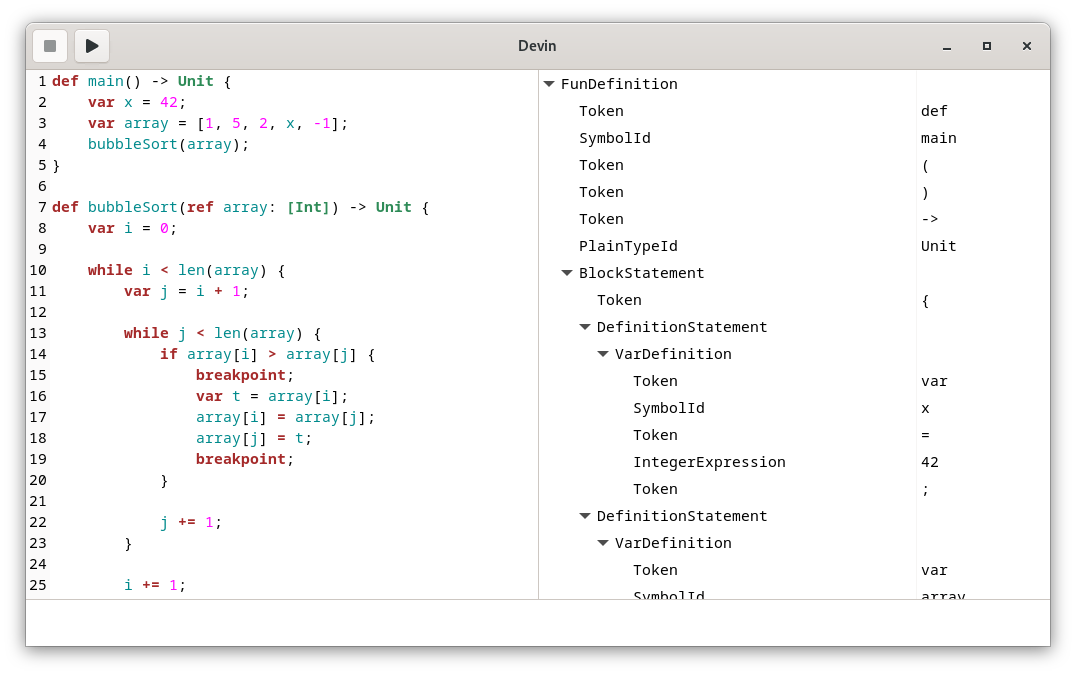
\includegraphics[width=0.9\textwidth]{2.png}
    \caption{The graphical editor associated with Devin}
  \end{figure}

  \newpage

  \section{Language features}

  Devin is an imperative programming language with lexical variable scoping and
  support for recursive function definitions. Syntactically, it's similar to any
  C descendant; among others, it supports variable definition and assignment,
  while loops, do-while loops and branching via if and if-else statements.

  \subsection{Data types}

  Devin features the following data types:

  \begin{itemize}
    \item \mbox{\texttt{Bool}}, for the boolean values \mbox{\texttt{true}},
    \mbox{\texttt{false}};

    \item \mbox{\texttt{Int}}, for 64-bit integers denoted by sequences of
    digits like \mbox{\texttt{42}};

    \item \mbox{\texttt{Float}}, for double-precision floating-point numbers
    like \mbox{\texttt{0.0}} and \mbox{\texttt{3.14}}. The presence of the
    fractional part distinguishes integers from floats. Contrary to C,
    exponential notation like \mbox{\texttt{1E100}} is not supported;

    \item \mbox{\texttt{[$T$]}}, for arrays like
    \mbox{\texttt{[1, 1, 2, 3, 5, 8, 13, 21, 34, 55]}}.
  \end{itemize}

  In addition to the items above, Devin has a unit type named
  \mbox{\texttt{Unit}}; it is inhabited by one value only: \mbox{\texttt{unit}}.
  When a function has side-effects only, it is marked as returning
  \mbox{\texttt{Unit}}.

  With unit types, there's no need to distinguish between functions that return
  a value and procedures that do not: all callables always return a value. One
  of the advantages of unit types is the uniform treatment of assignments. While
  unit types are traditionally used in functional programming languages, some
  recent imperative languages like Kotlin and Rust incorporate this feature as
  well.

  \subsection{Built-in operators}

  Booleans support the usual operations of negation, logical conjunction and
  disjunction. An operator for exclusive disjunction is provided as well.

  Boolean binary operations are evaluated lazily: the right operand is only
  evaluated if the left operand doesn't already determine the result of the
  whole expression.

  \begin{table}[H]
    \centering

    \begin{tabular}{|c|c|c|c|}
      \hline

      Description &
      Syntax &
      C equivalent &
      Semantic meaning \\
      \hline

      Negation &
      \texttt{not($p$)} &
      \texttt{!$p$} &
      $\lnot p$ \\

      Conjunction &
      \texttt{$p$ and $q$} &
      \texttt{$p$ \&\& $q$} &
      $p \land q$ \\

      Disjunction &
      \texttt{$p$ or $q$} &
      \texttt{$p$ || $q$} &
      $p \lor q$ \\

      Exclusive disjunction &
      \texttt{$p$ xor $q$} &
      \texttt{$p$ != $q$} &
      $\left(p \land \lnot q\right) \lor \left(\lnot p \land q\right)$ \\
      \hline
    \end{tabular}

    \caption{Boolean operators}
  \end{table}

  Integers and floating-point numbers support addition, subtraction,
  multiplication and division. For integers (but not floats), there's also a
  modulo operator.

  Binary arithmetic operations require both operands to be of the same numeric
  type: type conversions have to be performed explicitly via
  \mbox{\texttt{intToFloat($n$)}} and \mbox{\texttt{floatToInt($x$)}}.

  Division (operator \texttt{/}) behaves differently depending on the types of
  the operands. In any case, the result of arithmetic operations has the same
  type as their operands.

  \begin{table}[H]
    \centering

    \begin{tabular}{|c|c|c|}
      \hline

      Description &
      Syntax &
      Semantic meaning \\
      \hline

      Negation &
      \texttt{-$x$} &
      $-x$ \\

      Identity &
      \texttt{+$x$} &
      $+x$ \\

      Addition &
      \texttt{$x$ + $y$} &
      $x + y$ \\

      Subtraction &
      \texttt{$x$ - $y$} &
      $x - y$ \\

      Multiplication &
      \texttt{$x$ * $y$} &
      $x \times y$ \\

      Integer division &
      \texttt{$n$ / $m$} &
      $\lfloor n \div m \rfloor$ \\

      Floating-point division &
      \texttt{$x$ / $y$} &
      $x \div y$ \\

      Modulo &
      \texttt{$n$ \% $m$} &
      $n - m \times \lfloor n \div m \rfloor$ \\
      \hline
    \end{tabular}

    \caption{Arithmetic operators}
  \end{table}

  Values can be compared with the expressions \mbox{\texttt{$x$ < $y$}},
  \mbox{\texttt{$x$ <= $y$}}, \mbox{\texttt{$x$ > $y$}} and
  \mbox{\texttt{$x$ >= $y$}}. Equality and inequality between any two values can
  be tested with \mbox{\texttt{$x$ == $y$}} and \mbox{\texttt{$x$ != $y$}},
  respectively.

  \begin{table}[H]
    \centering

    \begin{tabular}{|c|c|c|}
      \hline

      Description &
      Syntax &
      Semantic meaning \\
      \hline

      \multirow{4}{*}{Comparison} &
      \texttt{$x$ > $y$} &
      $x < y$ \\

      &
      \texttt{$x$ <= $y$} &
      $x \leq y$ \\

      &
      \texttt{$x$ > $y$} &
      $x > y$ \\

      &
      \texttt{$x$ >= $y$} &
      $x \geq y$ \\

      \multirow{2}{*}{Equality} &
      \texttt{$x$ == $y$} &
      $x = y$ \\

      &
      \texttt{$x$ != $y$} &
      $x \neq y$ \\
      \hline
    \end{tabular}

    \caption{Relational operators}
  \end{table}

  Variables and array elements can be assigned using the \texttt{=} operator.
  Like many languages, Devin features a few shorthands as well.

  \begin{table}[H]
    \centering

    \begin{tabular}{|c|c|c|}
      \hline

      Description &
      Syntax &
      Semantic meaning \\
      \hline

      Plain assignment &
      \texttt{$x$ = $y$} &
      $x \leftarrow y$ \\

      \multirow{5}{*}{Assignment shorthand} &
      \texttt{$x$ += $y$} &
      \texttt{$x$ = $x$ + $y$} \\

      &
      \texttt{$x$ -= $y$} &
      \texttt{$x$ = $x$ - $y$} \\

      &
      \texttt{$x$ *= $y$} &
      \texttt{$x$ = $x$ * $y$} \\

      &
      \texttt{$x$ /= $y$} &
      \texttt{$x$ = $x$ / $y$} \\

      &
      \texttt{$x$ \%= $y$} &
      \texttt{$x$ = $x$ \% $y$} \\
      \hline
    \end{tabular}

    \caption{Assignment operators}
    \label{table:assignment-operators}
  \end{table}

  \newpage

  \subsection{Working with arrays}

  Arrays support the following operations:

  \begin{itemize}
    \item \emph{Element access}: \mbox{\texttt{$a$[$n$]}}, where $a$ denotes an
    array and $n$ an integer index. The expression retrieves the $n$-th element
    of the array. As in most programming languages, the first element of the
    array has index $0$.

    \item \emph{Length information}: \mbox{\texttt{len($a$)}}. This expression
    returns the number of elements contained in the array $a$.

    \item \emph{Concatenation}: \mbox{\texttt{$a$ + $b$}}. This expression
    yields a new array containing the elements of $a$ concatenated with the
    elements of $b$.

    \item \emph{Repetition}: \mbox{\texttt{$a$ * $n$}} or
    \mbox{\texttt{$n$ * $a$}}. Equivalent to concatenating $a$ to itself $n$
    times. \\
    Zero-initialized arrays of size $n$ can be generated with the expression
    \mbox{\texttt{[0] * $n$}}.
  \end{itemize}

  \subsection{Variable definitions and scoping}

  Variables can be defined using statements of the form
  \mbox{\texttt{var $x$ = $y$}}, where $x$ is an identifier and $y$ is an
  expression; the type of the new variable $x$ is inferred from $y$. Variables
  can be defined at any point, whether globally or as function locals; their
  visibility extends from the point of their definition onward.

  Devin is \emph{block-structured}: it allows for the creation of blocks,
  including blocks nested within other blocks. Variables are lexically scoped:
  they can't be accessed from outside the block they are defined in. As in C, a
  block consists of a sequence of statements wrapped between a pair of curly
  braces (\texttt{\{}, \texttt{\}}). Statements are always terminated with
  semicolons.

  \begin{Listing}[H]
    \begin{Verbatim}[gobble=6,fontsize=\small]
      def rotateRight(ref array) -> Unit {
          if len(array) > 0 {
              var i = len(array) - 1;
              var t = array[i];

              while i > 0 {
                  array[i] = array[i - 1];
                  i -= 1;
              }

              array[0] = t;
          }  // 'i', 't' go out of scope
      }  // 'array' goes out of scope
    \end{Verbatim}

    \caption{Devin's scoping rules visualized}
  \end{Listing}

  \newpage

  \subsection{Branching and looping mechanisms}

  The following two standard looping constructs are supported:

  \begin{itemize}
    \item \emph{While loops} in the form \mbox{\texttt{while $p$ $s$}}. This
    construct evaluates $p$; if it is \mbox{\texttt{true}}, $s$ is run. This
    repeats until $p$ evaluates to \mbox{\texttt{false}}.

    \item \emph{Do-while loops} in the form \mbox{\texttt{do $s$ while $p$}}.
    This construct runs $s$; this repeats unless a subsequent evaluation of $p$
    yields \mbox{\texttt{false}}.
  \end{itemize}

  Conditional code execution is supported through statements of the form
  \mbox{\texttt{if $p$ $s_1$}} and \mbox{\texttt{if $p$ $s_1$ else $s_2$}},
  where $p$ is a boolean expression and $s_1$ and $s_2$ are statements.

  \subsection{Assertions}

  Devin provides a mechanism for asserting that predicates evaluate to
  \mbox{\texttt{true}} at runtime; if they do not, an exception is raised,
  leading to program termination. Assertions can be used to check internal
  assumptions or to guard against violation of function contracts, among other
  things.

  For example, the assertion \mbox{\texttt{assert n >= 0}} can be used as the
  first statement of a function calculating the factorial of \texttt{n}, as the
  result is not defined if \mbox{$\mathtt{n} < 0$}.

  \subsection{Function definition and application}

  Functions can be defined either globally or within other functions. They
  adhere to the same scoping rules as variables. The entry point for Devin
  programs is a global function named \mbox{\texttt{main}}; it must take no
  arguments.

  The syntax for calling functions is the same as in C: \mbox{\texttt{$f$()}}
  calls $f$ with zero arguments, \mbox{\texttt{$g$($x$)}} calls $g$ with a
  single argument, \mbox{\texttt{$h$($x$, $y$)}} calls $h$ with two arguments,
  and so on.

  The evaluation strategy of Devin is eager; arguments are evaluated from left
  to right. By default, function arguments are passed by value; with the
  \mbox{\texttt{ref}} keyword, they can be passed by reference instead (see
  \autoref{listing:optional-types}).

  \subsection{Optional types}

  A peculiar feature of Devin is that of \emph{optional types}. With optional
  types, the semantics of the language doesn't depend on the static type
  system~\cite{pluggable-type-systems}. A notable example of an optionally typed
  language is Python. With this feature, type annotations can be omitted from
  Devin programs. Type checking is not performed on terms where type annotations
  are missing.

  \begin{Listing}[H]
    \begin{Verbatim}[gobble=6,fontsize=\small]
      def swap1(ref array: [Int], i: Int, j: Int) -> Unit {
          var t = array[i];
          array[i] = array[j];
          array[j] = t;
      }

      // Note: 'swap2' is more general than 'swap1', as it can be used with any array
      def swap2(ref array, i, j) {
          var t = array[i];
          array[i] = array[j];
          array[j] = t;
      }
    \end{Verbatim}

    \caption{Optional types exemplified}
    \label{listing:optional-types}
  \end{Listing}

  \section{Editor features}
  \label{section:editor-features}

  Devin comes with a code editing UI built on GTK+, a popular library for
  creating graphical user interfaces. GTK+ is compatible with Windows, macOS and
  many UNIX-like platforms~\cite{gtk+}. Code editing is facilitated by
  GtkSourceView, a library that extends the GTK+ framework to support text
  editing and configurable syntax highlighting~\cite{gtksourceview}.

  In addition to syntax highlighting, Devin's editor features error reporting:
  both syntactic and semantic errors are displayed according to their position
  in the source code.

  \begin{figure}[H]
    \centering
    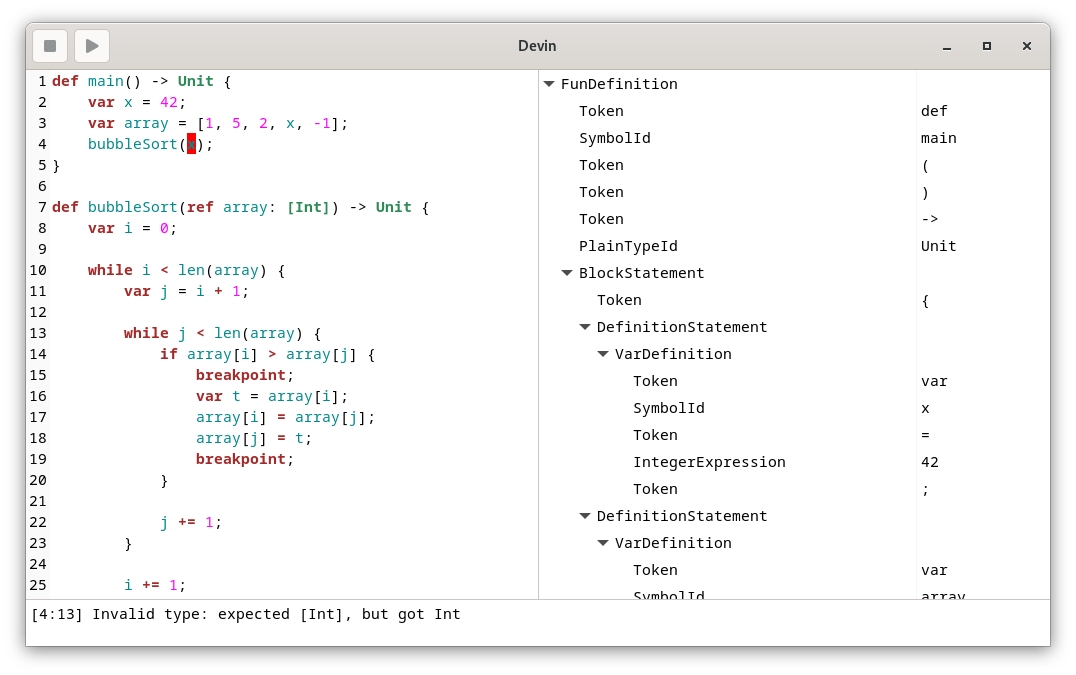
\includegraphics[width=0.9\textwidth]{4.png}
    \caption{Semantic error reporting and highlighting}
  \end{figure}

  \pagebreak

  Once a valid program is written, it can be executed by clicking the
  {\blacktriangleright} button. The execution state can be observed with
  breakpoint statements; these instruct the evaluator to pause execution and
  display the current runtime stack, as seen in \autoref{figure:debugger}. The
  execution stack, which maps variables and function arguments to their values,
  can be viewed from the user interface. Each function call pushes a new frame
  is onto the stack, containing associations between parameter names and their
  passed values. Variable definitions within the called function add new
  associations to the newly pushed frame. When the called function returns, the
  topmost frame is popped off the stack and execution continues normally.

  Devin has been designed with simplicity of implementation in mind. In
  particular, Devin's call stack exhibits two properties:

  \begin{itemize}
    \item Each block pushes a new frame onto the stack: this allows treating
    nested scopes with the same mechanism as function calls. The debugger hides
    this detail by displaying what appears to be a single frame for each call.

    \item Program execution always starts with a non-empty stack containing a
    single frame. This frame associates the name \mbox{\texttt{true}} to the
    truth value, \mbox{\texttt{false}} to \mbox{\texttt{not true}}, and
    \mbox{\texttt{unit}} to the unit value.

    In practice, this means that \mbox{\texttt{true}}, \mbox{\texttt{false}} and
    \mbox{\texttt{unit}} are not special keywords or constants; instead, they
    are ordinary variables. This is a deliberate design decision.
  \end{itemize}

  \begin{figure}[H]
    \centering
    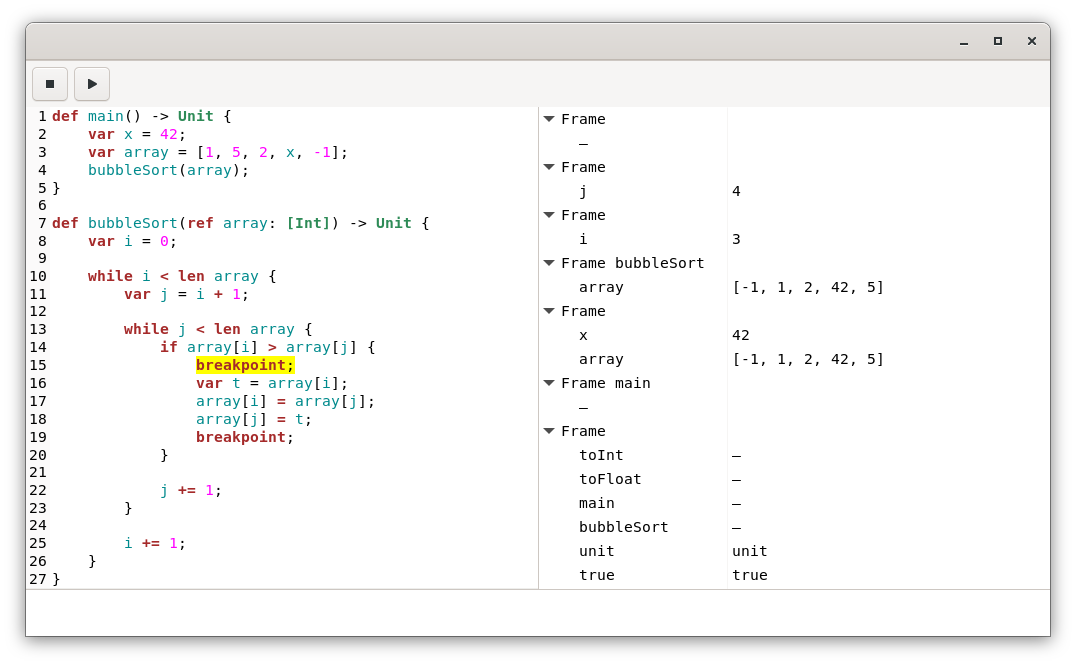
\includegraphics[width=0.9\textwidth]{5.png}
    \caption{The debugger displaying the current state of the stack}
    \label{figure:debugger}
  \end{figure}

  \pagebreak

  Runtime errors are handled as well. When an error occurs, the offending code
  fragment is highlighted and a descriptive message dialog is shown to the user.
  Runtime errors include, but are not limited to, index out of bounds errors,
  division by zero, assertion violations.

  \begin{figure}[H]
    \centering
    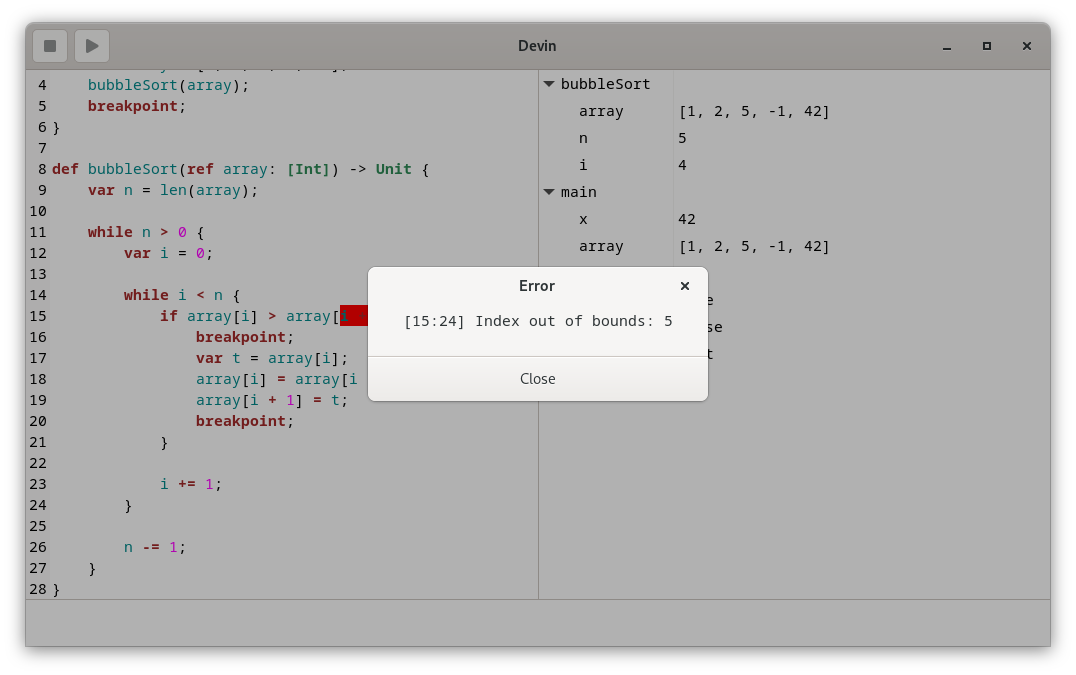
\includegraphics[width=0.9\textwidth]{6.png}
    \caption{Runtime error reporting and highlighting}
  \end{figure}

  \section{Devin's design choices}

  \subsection{Operations between numeric types}

  Addition, subtraction, multiplication, division and modulo are supported only
  if both operands are of the same numeric type. For instance, it isn't legal to
  add a floating-point number to an integer. While this restriction might seem
  unconventional at first, there is a very specific reason for it.

  In Devin, both integers and floating-point numbers occupy 64 bits. Adding two
  numbers of the same type $T$ yields yet another number of type $T$: nothing
  surprising here. But what should be the result of adding an integer to a
  floating-point number, or vice versa? Many languages take the approach of
  silently converting the integer operand to a floating-point value, and then
  performing the actual addition. Double-precision floating-point numbers as
  specified in IEEE 754 can't safely represent integers less than
  \mbox{$-\left(2^{53} - 1\right)$} or greater than \mbox{$2^{53} - 1$} without
  loss of precision~\cite{mdn-is-safe-integer}; as such, I argue that a
  programming language should make conversions between integers and floats
  explicit.

  This design decision is largely inspired by how Haskell deals with numbers.
  Examples of other languages which lack implicit conversions are
  Go~\cite{go-numeric-types} and Rust~\cite{rust-conversion}.

  \subsection{Optional types}

  As discussed previously, type annotations may be omitted at will. As Devin's
  type checker and evaluator are independent, optional types \emph{emerged} as a
  possible additional feature.

  Much can be said regarding the benefits and drawbacks of optional types. Devin
  was born due to my own curiosity regarding programming languages and their
  implementation; recreating the next Pascal or C clone is not an objective. As
  optional types are not a common feature, and as languages shape the way we
  think about solving problems, I decided to add this feature to be played
  around with.

  \newpage
  \thispagestyle{empty}

  \chapter{Implementing Devin}

  Devin's implementation spans almost 3700 lines of code and is entirely written
  in Haskell. Given the size of its implementation, some details are omitted for
  brevity. In particular, import declarations and \mbox{\texttt{LANGUAGE}}
  pragmas are left out for simplicity. Note that some of the functionality of
  the package \mbox{\texttt{extra}} is used: the library provides extra
  functions for the standard Haskell libraries, filling out missing
  functionality~\cite{extra}. Devin's full implementation can be found in the
  \hyperref[chapter:devin-source-code]{appendix}.

  In terms of implementation complexity, both the type checker and the evaluator
  are somewhat simpler than the parser. The parser makes much greater use of
  higher-order functions and uses multi-parameter type classes, causing some
  syntactical noise on function signatures; for this reason, I'll describe
  parsing last.

  \section{The syntax tree}

  Devin's syntax tree stores enough information to perform syntax highlighting.
  Given a node in the tree, it is always possible to determine its position
  within the parsed source code. Only leaf nodes store their positions directly;
  the positions of non-leaf nodes can be computed by considering their first and
  last children.

  Two leaf nodes commonly used across Devin's syntax tree are
  \mbox{\texttt{SymbolId}} and \mbox{\texttt{Token}}. They store information
  about identifiers (e.g., \texttt{x}, \mbox{\texttt{Int}}) and tokens (e.g.,
  \texttt{\{}, \texttt{\}}, \mbox{\texttt{->}}), respectively. They are defined
  as follows:

  \begin{Verbatim}[gobble=4,fontsize=\small]
    data SymbolId = SymbolId { name :: String, interval :: (Int, Int) }

    data Token = Token { interval :: (Int, Int) }
  \end{Verbatim}

  \newpage

  \subsection{Representing expressions}

  Literals, numbers and variables are the simplest kinds of expressions, as they
  are leaves in the syntax tree. More complex expressions can be built from
  simpler ones: for example, a binary expression is constructed by two
  sub-expressions and a binary operator.

  The pair of unary operators \texttt{+} and \texttt{-}, along with the 20
  binary operators \texttt{+}, \texttt{-}, \texttt{*}, \texttt{/}, \texttt{\%},
  \mbox{\texttt{==}}, \mbox{\texttt{!=}}, \texttt{<}, \mbox{\texttt{<=}},
  \texttt{>}, \mbox{\texttt{>=}}, \mbox{\texttt{and}}, \mbox{\texttt{or}},
  \mbox{\texttt{xor}}, \texttt{=}, \mbox{\texttt{+=}}, \mbox{\texttt{-=}},
  \mbox{\texttt{*=}}, \mbox{\texttt{/=}}, \mbox{\texttt{\%=}} are represented by
  the algebraic data types \mbox{\texttt{UnaryOperator}} and
  \mbox{\texttt{BinaryOperator}}, respectively:

  \begin{Verbatim}[gobble=4,fontsize=\small]
    data UnaryOperator
      = PlusOperator { interval :: (Int, Int) }
      | MinusOperator { interval :: (Int, Int) }

    data BinaryOperator
      = AddOperator { interval :: (Int, Int) }
      | SubtractOperator { interval :: (Int, Int) }
      | MultiplyOperator { interval :: (Int, Int) }
      | DivideOperator { interval :: (Int, Int) }
      | ModuloOperator { interval :: (Int, Int) }
      | EqualOperator { interval :: (Int, Int) }
      | NotEqualOperator { interval :: (Int, Int) }
      | LessOperator { interval :: (Int, Int) }
      | LessOrEqualOperator { interval :: (Int, Int) }
      | GreaterOperator { interval :: (Int, Int) }
      | GreaterOrEqualOperator { interval :: (Int, Int) }
      | AndOperator { interval :: (Int, Int) }
      | OrOperator { interval :: (Int, Int) }
      | XorOperator { interval :: (Int, Int) }
      | PlainAssignOperator { interval :: (Int, Int) }
      | AddAssignOperator { interval :: (Int, Int) }
      | SubtractAssignOperator { interval :: (Int, Int) }
      | MultiplyAssignOperator { interval :: (Int, Int) }
      | DivideAssignOperator { interval :: (Int, Int) }
      | ModuloAssignOperator { interval :: (Int, Int) }
  \end{Verbatim}

  Expressions are represented by a single algebraic data type:
  \mbox{\texttt{Expression}}. Opening and closing parentheses are stored in the
  syntax tree. As a convention, parentheses are always identified by the
  \mbox{\texttt{open}} and \mbox{\texttt{close}} fields, regardless of the kind:
  round, square, or curly.

  \begin{Verbatim}[gobble=4,fontsize=\small]
    data Expression where
      VarExpression :: {
        varName :: String,
        interval :: (Int, Int)
      } -> Expression

      IntegerExpression :: {
        integer :: Integer,
        interval :: (Int, Int)
      } -> Expression
  \end{Verbatim}

  \pagebreak

  \begin{Verbatim}[gobble=4,fontsize=\small]
      RationalExpression :: {
        rational :: Rational,
        interval :: (Int, Int)
      } -> Expression

      ArrayExpression :: {
        open :: Token,
        elems :: [Expression],
        commas :: [Token],
        close :: Token
      } -> Expression

      AccessExpression :: {
        array :: Expression,
        open :: Token,
        index :: Expression,
        close :: Token
      } -> Expression

      CallExpression :: {
        funId :: SymbolId,
        open :: Token,
        args :: [Expression],
        commas :: [Token],
        close :: Token
      } -> Expression

      UnaryExpression :: {
        unary :: UnaryOperator,
        operand :: Expression
      } -> Expression

      BinaryExpression :: {
        left :: Expression,
        binary :: BinaryOperator,
        right :: Expression
      } -> Expression

      ParenthesizedExpression :: {
        open :: Token,
        inner :: Expression,
        close :: Token
      } -> Expression
  \end{Verbatim}

  \subsection{Representing statements}

  Any expression followed by a semicolon is a statement. These expression
  statements are represented by the algebraic data type
  \mbox{\texttt{Statement}}, along with if, if-else, while, do-while, return,
  assert, breakpoint, and block statements.

  \pagebreak

  At any point in which a statement can occur, a variable or function definition
  may be placed instead. The data constructor
  \mbox{\texttt{DefinitionStatement}} represents this idea.

  \begin{Verbatim}[gobble=4,fontsize=\small]
    data Statement where
      DefinitionStatement :: {
        definition :: Definition
      } -> Statement

      ExpressionStatement :: {
        effect :: Expression,
        semicolon :: Token
      } -> Statement

      IfStatement :: {
        ifKeyword :: Token,
        predicate :: Expression,
        trueBranch :: Statement
      } -> Statement

      IfElseStatement :: {
        ifKeyword :: Token,
        predicate :: Expression,
        trueBranch :: Statement,
        elseKeyword :: Token,
        falseBranch :: Statement
      } -> Statement

      WhileStatement :: {
        whileKeyword :: Token,
        predicate :: Expression,
        body :: Statement
      } -> Statement

      DoWhileStatement :: {
        doKeyword :: Token,
        body :: Statement,
        whileKeyword :: Token,
        predicate :: Expression,
        semicolon :: Token
      } -> Statement

      ReturnStatement :: {
        returnKeyword :: Token,
        result :: Maybe Expression,
        semicolon :: Token
      } -> Statement

      AssertStatement :: {
        assertKeyword :: Token,
        predicate :: Expression,
        semicolon :: Token
      } -> Statement
  \end{Verbatim}

  \pagebreak

  \begin{Verbatim}[gobble=4,fontsize=\small]
      BreakpointStatement :: {
        breakpointKeyword :: Token,
        semicolon :: Token
      } -> Statement

      BlockStatement :: {
        open :: Token,
        statements :: [Statement],
        close :: Token
      } -> Statement
  \end{Verbatim}

  \subsection{Representing variable and function definitions}

  Devin's function definitions may or may not include signatures with explicit
  types. The syntax for array types involves a type enclosed in square brackets,
  as in \mbox{\texttt{[Int]}} or \mbox{\texttt{[[Float]]}}; the arbitrary
  syntactical nesting of paired square brackets around a type is permitted by
  the algebraic data type \mbox{\texttt{TypeId}}:

  \begin{Verbatim}[gobble=4,fontsize=\small]
    data TypeId
      = PlainTypeId { name :: String, interval :: (Int, Int) }
      | ArrayTypeId { open :: Token, innerTypeId :: TypeId, close :: Token }
  \end{Verbatim}

  Variables and function definitions are represented by
  \mbox{\texttt{VarDefinition}} and \mbox{\texttt{FunDefinition}}:

  \begin{Verbatim}[gobble=4,fontsize=\small]
    data Definition where
      VarDefinition :: {
        varKeyword :: Token,
        varId :: SymbolId,
        equalSign :: Token,
        value :: Expression,
        semicolon :: Token
      } -> Definition

      FunDefinition :: {
        defKeyword :: Token,
        funId :: SymbolId,
        open :: Token,
        params :: [(Maybe Token, SymbolId, Maybe (Token, TypeId))],
        commas :: [Token],
        close :: Token,
        returnInfo :: Maybe (Token, TypeId),
        body :: Statement
      } -> Definition
  \end{Verbatim}

  \section{Representing semantic errors}

  Both the evaluator and the type checker benefit from having a data type to
  represent errors. Runtime errors, such as division by zero, are raised by the
  evaluator. Static analysis errors, like missing return statements, are
  reported by the type checker. Since some errors are common to both phases, a
  single algebraic data type is used:

  \begin{Verbatim}[gobble=4,fontsize=\small]
    data Error where
      UnknownVar :: {
        varName :: String,
        interval :: (Int, Int)
      } -> Error

      UnknownFun :: {
        funName :: String,
        interval :: (Int, Int)
      } -> Error

      UnknownType :: {
        typeName :: String,
        interval :: (Int, Int)
      } -> Error

      InvalidUnary :: {
        unary :: UnaryOperator,
        operandT :: Type
      } -> Error

      InvalidBinary :: {
        binary :: BinaryOperator,
        leftT :: Type,
        rightT :: Type
      } -> Error

      InvalidType :: {
        expression :: Expression,
        expectedT :: Type,
        actualT :: Type
      } -> Error

      -- Static errors:

      MissingReturnValue :: {
        statement :: Statement,
        expectedT :: Type
      } -> Error

      MissingReturnStatement :: {
        funId :: SymbolId
      } -> Error

      -- Runtime errors:

      IntegerOverflow :: {
        expression :: Expression
      } -> Error
  \end{Verbatim}

  \pagebreak

  \begin{Verbatim}[gobble=4,fontsize=\small]
      DivisionByZero :: {
        expression :: Expression
      } -> Error

      IndexOutOfBounds :: {
        expression :: Expression,
        value :: Int64
      } -> Error

      InvalidArgCount :: {
        expression :: Expression,
        expected :: Int,
        actual :: Int
      } -> Error

      AssertionFailed :: {
        statement :: Statement
      } -> Error
  \end{Verbatim}

  \section{The type checker}

  Type checking is performed by a set of functions that operate on an
  \emph{environment}: a data structure associating identifiers with types. The
  environment is used to verify if function calls and variable usages are valid
  within their context.

  The module \mbox{\texttt{Devin.Type}} provides the necessary data types to
  represent types themselves. The data constructors \mbox{\texttt{Unit}},
  \mbox{\texttt{Bool}}, \mbox{\texttt{Int}}, \mbox{\texttt{Float}} and
  \mbox{\texttt{Array}} correspond to Devin's supported types. To aid the type
  checker, two other data constructors are provided, both indicating some sort
  of error: \mbox{\texttt{Unknown}} and \mbox{\texttt{Placeholder}}. While
  \mbox{\texttt{Unknown}} stands for an unknown type,
  \mbox{\texttt{Placeholder}} represents a specific unresolved type.
  Differentiating between \mbox{\texttt{Placeholder}} and
  \mbox{\texttt{Unknown}} allows for fine-grained error messages and
  diagnostics. For instance, if a misspelled type occurs the same way $n$ times
  within some scope, it corresponds to \emph{one}, instead of $n$, type errors.

  \begin{Verbatim}[gobble=4,fontsize=\small]
    data Type
      = Unknown
      | Unit
      | Bool
      | Int
      | Float
      | Array Type
      | Placeholder String
  \end{Verbatim}

  To compare types, the relation operator \mbox{\texttt{(<:)}} is provided:

  \begin{Verbatim}[gobble=4,fontsize=\small]
    (<:) :: Type -> Type -> Bool
    t1 <: t2 = isJust (merge t1 t2)
  \end{Verbatim}

  \pagebreak

  \begin{Verbatim}[gobble=4,fontsize=\small]
    merge :: Type -> Type -> Maybe Type
    merge Unknown _ = Just Unknown
    merge _ Unknown = Just Unknown
    merge Unit Unit = Just Unit
    merge Bool Bool = Just Bool
    merge Int Int = Just Int
    merge Float Float = Just Float
    merge (Array t1) (Array t2) = Array <$> merge t1 t2
    merge (Placeholder n1) (Placeholder n2) | n1 == n2 = Just (Placeholder n1)
    merge _ _ = Nothing
  \end{Verbatim}

  Given two types, the helper function \mbox{\texttt{merge}} yields a type that
  is compatible with both, if possible. All types except for
  \mbox{\texttt{Unknown}} are only compatible with themselves;
  \mbox{\texttt{Unknown}}, on the other hand, is compatible with all other
  types.

  The module \mbox{\texttt{Devin.Typer}} implements the type checker interface.
  To account for Devin's lexical scoping rules, the environment is represented
  as a list of association lists.

  \begin{Verbatim}[gobble=4,fontsize=\small]
    data Scope = Scope {
      types :: [(String, Type)],
      funs :: [(String, ([Type], Type))],
      vars :: [(String, Type)]
    }

    type Environment = [Scope]

    data Typer a = Typer { runTyper :: Environment -> (a, Environment, [Error]) }
      deriving Functor

    predefinedEnv :: Environment
    predefinedEnv =
      let t1 = ("Unit", Unit)
          t2 = ("Bool", Bool)
          t3 = ("Int", Int)
          t4 = ("Float", Float)

          f1 = ("not", ([Bool], Bool))
          f2 = ("len", ([Array Unknown], Int))
          f3 = ("intToFloat", ([Int], Float))
          f4 = ("floatToInt", ([Float], Int))

          v1 = ("true", Bool)
          v2 = ("false", Bool)
          v3 = ("unit", Unit)

       in [Scope [t4, t3, t2, t1] [f4, f3, f2, f1] [v3, v2, v1]]
  \end{Verbatim}

  In the listing above, \mbox{\texttt{Typer}} wraps a function that takes an
  \mbox{\texttt{Environment}} and returns a new environment and a potentially
  empty list of \mbox{\texttt{Error}s}, along with a result of some kind.
  \mbox{\texttt{deriving Functor}} instructs GHC to automatically generate an
  implementation for the function
  \mbox{\texttt{fmap :: (a -> b) -> Typer a -> Typer b}}.

  Below, implementations for \mbox{\texttt{pure}}, \mbox{\texttt{liftA2}},
  \mbox{\texttt{(>>=)}} are provided. These functions, in conjunction with
  \mbox{\texttt{fmap}}, render \mbox{\texttt{Typer}} a monad.

  \begin{Verbatim}[gobble=4,fontsize=\small]
    instance Applicative Typer where
      pure :: a -> Typer a
      pure x = Typer (\env -> (x, env, []))

      liftA2 :: (a -> b -> c) -> Typer a -> Typer b -> Typer c
      liftA2 f mx my = Typer $ \env ->
        let (x, env', errors1) = runTyper mx env
            (y, env'', errors2) = runTyper my env'
         in (f x y, env'', errors1 ++ errors2)

    instance Monad Typer where
      (>>=) :: Typer a -> (a -> Typer b) -> Typer b
      mx >>= f = Typer $ \env ->
        let (x, env', errors1) = runTyper mx env
            (y, env'', errors2) = runTyper (f x) env'
         in (y, env'', errors1 ++ errors2)
  \end{Verbatim}

  Some utility functions are defined. \mbox{\texttt{defineType}} binds a type
  name (such as \mbox{\texttt{"Unit"}}) to a \mbox{\texttt{Type}} (such as
  \mbox{\texttt{Unit}}); the binding is added to the current environment. Its
  counterpart, \mbox{\texttt{lookupType}}, looks up the type to which a name is
  bound. \mbox{\texttt{lookupType}} searches the current environment; if no
  binding is found, the parent environment is scanned next.

  \begin{Verbatim}[gobble=4,fontsize=\small]
    defineType :: String -> Type -> Typer Type
    defineType name t = Typer $ \case
      [] -> (t, [Scope [(name, t)] [] []], [])

      scope : scopes ->
        let types' = (name, t) : types scope
         in (t, scope{types = types'} : scopes, [])

    lookupType :: String -> Typer (Maybe (Type, Int))
    lookupType name = Typer (\env -> (go 0 env, env, []))
      where
        go _ [] = Nothing

        go depth (Scope{types} : scopes) = case lookup name types of
          Just t -> Just (t, depth)
          Nothing -> go (depth + 1) scopes
  \end{Verbatim}

  An expression of the form
  \mbox{\texttt{\textbackslash case \{ $p_1$ -> $e_1$; $\ldots$; $p_n$ -> $e_n$ \}}}
  is called a \emph{lambda-case}; it is equivalent to
  \mbox{\texttt{\textbackslash $x$ -> case $x$ of \{ $p_1$ -> $e_1$; $\ldots$; $p_n$ -> $e_n$ \}}},
  where $x$ is a fresh variable. Lambda-case syntax is enabled by the
  \mbox{\texttt{LambdaCase}} language extension.

  Next, the functions \mbox{\texttt{defineFunSignature}} and
  \mbox{\texttt{lookupFunSignature}} define and lookup associations between
  names and function signatures, represented by a
  \mbox{\texttt{([Type], Type)}}. The first element of the tuple is the list of
  parameter types, the second is the return type.

  \pagebreak

  \begin{Verbatim}[gobble=4,fontsize=\small]
    defineFunSignature :: String -> ([Type], Type) -> Typer ()
    defineFunSignature name signature = Typer $ \case
      [] -> ((), [Scope [] [(name, signature)] []], [])

      scope : scopes ->
        let funs' = (name, signature) : funs scope
         in ((), scope{funs = funs'} : scopes, [])

    lookupFunSignature :: String -> Typer (Maybe (([Type], Type), Int))
    lookupFunSignature name = Typer (\env -> (go 0 env, env, []))
      where
        go _ [] = Nothing

        go depth (Scope{funs} : scopes) = case lookup name funs of
          Just signature -> Just (signature, depth)
          Nothing -> go (depth + 1) scopes
  \end{Verbatim}

  Finally, variables can be defined and looked up with
  \mbox{\texttt{defineVarType}} and \mbox{\texttt{lookupVarType}}.

  \begin{Verbatim}[gobble=4,fontsize=\small]
    defineVarType :: String -> Type -> Typer ()
    defineVarType name t = Typer $ \case
      [] -> ((), [Scope [] [] [(name, t)]], [])

      scope : scopes ->
        let vars' = (name, t) : vars scope
         in ((), scope{vars = vars'} : scopes, [])

    lookupVarType :: String -> Typer (Maybe (Type, Int))
    lookupVarType name = Typer (\env -> (go 0 env, env, []))
      where
        go _ [] = Nothing

        go depth (Scope{vars} : scopes) = case lookup name vars of
          Just t -> Just (t, depth)
          Nothing -> go (depth + 1) scopes
  \end{Verbatim}

  Functions for removing previously defined associations could be implemented;
  however, this is not necessary. Instead, the function
  \mbox{\texttt{withNewScope}} is provided to run another \mbox{\texttt{Typer}}
  in a modified environment where an empty \mbox{\texttt{Scope}} is added; when
  the function returns, the previous environment is restored.

  \begin{Verbatim}[gobble=4,fontsize=\small]
    withNewScope :: Typer a -> Typer a
    withNewScope mx = Typer $ \env ->
      let (x, env', errors) = runTyper mx (Scope [] [] [] : env)
       in (x, tail env', errors)
  \end{Verbatim}

  One last function is provided for utility: \mbox{\texttt{report}}. As its name
  suggests, this function reports some \mbox{\texttt{Error}}; errors are
  accumulated by the \mbox{\texttt{Typer}} monad and can be used in successive
  phases for error reporting and highlighting.

  \begin{Verbatim}[gobble=4,fontsize=\small]
    report :: Error -> Typer ()
    report error = Typer (\env -> ((), env, [error]))
  \end{Verbatim}

  \newpage

  \subsection{Checking expressions}

  Expression-related type checking is implemented in the
  \mbox{\texttt{Devin.Typers}} module with the
  \mbox{\texttt{checkExpression :: Expression -> Typer Type}} function.

  Devin has a rudimentary mechanism for type inference. The type of literal
  expressions is trivially determined by the kind of literal. For variables, a
  lookup in the current environment is performed; if the variable is not bound,
  an error is reported.

  \begin{Verbatim}[gobble=4,fontsize=\small]
    checkExpression IntegerExpression{} = pure Int

    checkExpression RationalExpression{} = pure Float

    checkExpression VarExpression{varName, interval} =
      lookupVarType varName >>= \case
        Just (t, _) -> pure t

        Nothing -> do
          report (UnknownVar varName interval)
          pure Unknown
  \end{Verbatim}

  For simplicity, the function \mbox{\texttt{report'}} is provided for future
  use. It is similar to \mbox{\texttt{report}}, but its result wraps
  \mbox{\texttt{Unknown}} instead of the unit type \mbox{\texttt{()}}.

  \begin{Verbatim}[gobble=4,fontsize=\small]
    report' :: Error -> Typer Type
    report' error = do
      report error
      pure Unknown
  \end{Verbatim}

  Inferring the type of arrays requires special care. In general, the type of an
  array is represented by \mbox{\texttt{Array $T$}}. If all elements of the
  array have the same type \mbox{$T_0$}, then $T$ can be determined to be
  \mbox{$T_0$}. If there are at least two elements of the array with different
  types, then $T$ can't be inferred.

  \begin{Verbatim}[gobble=4,fontsize=\small]
    checkExpression ArrayExpression{elems = elem : elems} = do
      t <- checkExpression elem

      flip loopM elems $ \case
        [] -> pure (Right (Array t))

        elem : elems -> checkExpression elem >>= \case
          Unknown -> do
            for_ elems checkExpression
            pure (Right (Array Unknown))

          t' | t' <: t -> pure (Left elems)

          t' -> do
            report (InvalidType elem t t')
            pure (Left elems)
  \end{Verbatim}

  The higher-order function
  \mbox{\texttt{loopM :: Monad m => (a -> m (Either a b)) -> a -> m b}}
  expresses a monadic loop operation where the predicate returns
  \mbox{\texttt{Left}} as a seed for the next loop, or \mbox{\texttt{Right}} to
  abort the loop. To apply \mbox{\texttt{loopM}} with flipped argument order,
  \mbox{\texttt{flip :: (a -> b -> c) -> b -> a -> c}} is used.

  As a special case, the type of an array can't be inferred when it is empty. To
  allow empty arrays to be used, no error is reported in such instance.

  \begin{Verbatim}[gobble=4,fontsize=\small]
    checkExpression ArrayExpression{elems = []} = pure (Array Unknown)
  \end{Verbatim}

  Access to array elements is checked as follows:

  \begin{Verbatim}[gobble=4,fontsize=\small]
    checkExpression AccessExpression{array, index} = do
      arrayT <- checkExpression array
      indexT <- checkExpression index

      case (arrayT, indexT) of
        (Unknown, Unknown) -> pure Unknown
        (Unknown, Int) -> pure Unknown
        (Unknown, _) -> report' (InvalidType index Int indexT)
        (Array t, Unknown) -> pure t
        (Array t, Int) -> pure t
        (Array _, _) -> report' (InvalidType index Int indexT)
        (_, _) -> report' (InvalidType array (Array Unknown) arrayT)
  \end{Verbatim}

  Unary arithmetic expressions with the operators \texttt{+} and \texttt{-} are
  type checked by ensuring that the operand is of a numeric type. If it is, the
  result of evaluating the whole expression has the same type as the operand.

  \begin{Verbatim}[gobble=4,fontsize=\small]
    checkExpression UnaryExpression{unary, operand}
      | PlusOperator{} <- unary = do
        operandT <- checkExpression operand

        case operandT of
          Unknown -> pure Unknown
          Int -> pure Int
          Float -> pure Float
          _ -> report' (InvalidUnary unary operandT)

    checkExpression UnaryExpression{unary, operand}
      | MinusOperator{} <- unary = do
        operandT <- checkExpression operand

        case operandT of
          Unknown -> pure Unknown
          Int -> pure Int
          Float -> pure Float
          _ -> report' (InvalidUnary unary operandT)
  \end{Verbatim}

  There is a certain degree of code repetition within Devin's type checker.
  While \emph{DRY} (Don't Repeat Yourself) is generally a good software
  development practice, it does become impractical when edge cases have to be
  considered. For instance, while both binary operators \texttt{+} and
  \texttt{-} operate on arithmetic types, \texttt{+} also works with arrays.
  Worse, in the evaluator, both \texttt{+} and \mbox{\texttt{and}} compute some
  result based on their operands, but the evaluation strategy of
  \mbox{\texttt{and}} differs from that of \texttt{+}. Source code could
  certainly be rearranged to avoid some amount of repetition; however, it would
  become less readable to some extent.

  What follows is the implementation to type check expressions with the binary
  operator~\texttt{/}. Both operands have to be of the same type; if they are,
  the result of evaluating the whole expression has the same type as the
  operands.

  \begin{Verbatim}[gobble=4,fontsize=\small]
    checkExpression BinaryExpression{left, binary, right}
      | DivideOperator{} <- binary = do
        leftT <- checkExpression left
        rightT <- checkExpression right

        case (leftT, rightT) of
          (Unknown, _) -> pure Unknown
          (_, Unknown) -> pure Unknown
          (Int, Int) -> pure Int
          (Float, Float) -> pure Float
          (_, _) -> report' (InvalidBinary binary leftT rightT)
  \end{Verbatim}

  The binary operators \texttt{-} and \texttt{\%} are type checked similarly to
  \texttt{/}, except for the fact that \texttt{\%} only accepts operands of type
  \mbox{\texttt{Int}}.

  The semantic meaning of the binary operator \texttt{+} depends on the type of
  the operands. If both are numeric, the operator denotes arithmetic addition;
  if the operands are arrays, \texttt{+} stands for array concatenation.
  Similarly, \texttt{*} could indicate both numeric multiplication and array
  repetition. As these operators are overloaded, all possibilities have to be
  considered during type checking.

  \begin{Verbatim}[gobble=4,fontsize=\small]
    checkExpression BinaryExpression{left, binary, right}
      | AddOperator{} <- binary = do
        leftT <- checkExpression left
        rightT <- checkExpression right

        case (leftT, rightT) of
          (Unknown, _) -> pure Unknown
          (_, Unknown) -> pure Unknown
          (Int, Int) -> pure Int
          (Float, Float) -> pure Float
          (Array t1, Array t2) | Just t <- merge t1 t2 -> pure (Array t)
          (_, _) -> report' (InvalidBinary binary leftT rightT)

    checkExpression BinaryExpression{left, binary, right}
      | MultiplyOperator{} <- binary = do
        leftT <- checkExpression left
        rightT <- checkExpression right
  \end{Verbatim}

  \pagebreak

  \begin{Verbatim}[gobble=4,fontsize=\small]
        case (leftT, rightT) of
          (Unknown, _) -> pure Unknown
          (_, Unknown) -> pure Unknown
          (Int, Int) -> pure Int
          (Float, Float) -> pure Float
          (Array t, Int) -> pure (Array t)
          (Int, Array t) -> pure (Array t)
          (_, _) -> report' (InvalidBinary binary leftT rightT)
  \end{Verbatim}

  Values can be compared with the binary operators \mbox{\texttt{==}},
  \mbox{\texttt{!=}}, \texttt{<}, \mbox{\texttt{<=}}, \texttt{>} and
  \mbox{\texttt{>=}}. Type checking ensures that both operands are of the same
  type; if they are, expressions with such operators yield a
  \mbox{\texttt{Bool}}; as we'll see, the semantic meaning of comparing
  non-numeric values is lexicographic ordering. Type checking is implemented in
  the same way for all six comparison operators:

  \begin{Verbatim}[gobble=4,fontsize=\small]
    checkExpression BinaryExpression{left, binary, right}
      | LessOperator{} <- binary = do
        leftT <- checkExpression left
        rightT <- checkExpression right

        case (leftT, rightT) of
          (Unknown, _) -> pure Unknown
          (_, Unknown) -> pure Unknown
          (_, _) | Just _ <- merge leftT rightT -> pure Bool
          (_, _) -> report' (InvalidBinary binary leftT rightT)
  \end{Verbatim}

  The operators \mbox{\texttt{and}}, \mbox{\texttt{or}} and \mbox{\texttt{xor}}
  are all type checked in the same way:

  \begin{Verbatim}[gobble=4,fontsize=\small]
    checkExpression BinaryExpression{left, binary, right}
      | AndOperator{} <- binary = do
        leftT <- checkExpression left
        rightT <- checkExpression right

        case (leftT, rightT) of
          (Unknown, _) -> pure Unknown
          (_, Unknown) -> pure Unknown
          (Bool, Bool) -> pure Bool
          (_, _) -> report' (InvalidBinary binary leftT rightT)
  \end{Verbatim}

  Plain assignment expressions with \texttt{=} are checked by verifying that
  both the left and right operands are of the same type:

  \begin{Verbatim}[gobble=4,fontsize=\small]
    checkExpression BinaryExpression{left, binary, right}
      | PlainAssignOperator{} <- binary = do
        leftT <- checkExpression left
        rightT <- checkExpression right

        if rightT <: leftT then
          pure rightT
        else
          report' (InvalidBinary binary leftT rightT)
  \end{Verbatim}

  Expressions with the binary operators \mbox{\texttt{+=}}, \mbox{\texttt{-=}},
  \mbox{\texttt{*=}}, \mbox{\texttt{/=}} and \mbox{\texttt{\%=}} are type
  checked considering the shorthands detailed in
  \autoref{table:assignment-operators}.

  The type resulting from function invocations is determined by looking up the
  callee's signature. If a call refers to an unbound identifier, or if the wrong
  number of arguments is provided, or if an argument has the wrong type, an
  error is reported.

  \begin{Verbatim}[gobble=4,fontsize=\small]
    checkExpression expression@CallExpression{funId, args} = do
      let SymbolId{name, interval} = funId

      lookupFunSignature name >>= \case
        Nothing -> report' (UnknownFun name interval)

        Just ((paramTs, returnT), _) -> go 0 args paramTs
          where
            go _ [] [] = pure returnT

            go n (arg : args) (paramT : paramTs) = do
              argT <- checkExpression arg
              unless (argT <: paramT) (report (InvalidType arg paramT argT))
              go (n + 1) args paramTs

            go n args paramTs = do
              let expected = n + length paramTs
              let actual = n + length args
              report' (InvalidArgCount expression expected actual)
  \end{Verbatim}

  \subsection{Checking statements}

  The function \mbox{\texttt{checkStatement :: Type -> Statement -> Typer Bool}}
  performs type checking on statements. A type must be provided: on return
  statements, \mbox{\texttt{checkStatement}} verifies that the returned value is
  of the given type.

  Inside functions, return statements may signal control to be returned to the
  callee. The function \mbox{\texttt{checkStatement}} wraps a
  \mbox{\texttt{Bool}} which is \mbox{\texttt{True}} if control is guaranteed to
  be returned to the callee and \mbox{\texttt{False}} otherwise.

  Expression and definition statements are trivial to check. In both cases, type
  checking is delegated to the relevant function.
  \mbox{\texttt{checkDefinitions}} is defined in the next section.

  \begin{Verbatim}[gobble=4,fontsize=\small]
    checkStatement _ ExpressionStatement{effect} = do
      checkExpression effect
      pure False

    checkStatement _ DefinitionStatement{definition} = do
      checkDefinitions [definition]
      pure False
  \end{Verbatim}

  \pagebreak

  For breakpoint statements, nothing needs to be done:

  \begin{Verbatim}[gobble=4,fontsize=\small]
    checkStatement _ BreakpointStatement{} = pure False
  \end{Verbatim}

  If-else statements are checked by ensuring that the predicate is a boolean
  expression and by recursively type checking both potential execution paths. We
  adopt a conservative approach, verifying if both branches return control; if
  so, the whole if-else statement surely must return control as well.

  \begin{Verbatim}[gobble=4,fontsize=\small]
    checkStatement expectedT IfElseStatement{predicate, trueBranch, falseBranch} = do
      t <- checkExpression predicate
      unless (t <: Bool) (report (InvalidType predicate Bool t))
      trueBranchDoesReturn <- withNewScope (checkStatement expectedT trueBranch)
      falseBranchDoesReturn <- withNewScope (checkStatement expectedT falseBranch)
      pure (trueBranchDoesReturn && falseBranchDoesReturn)
  \end{Verbatim}

  For if statements without an \mbox{\texttt{else}} clause, we follow the same
  conservative approach: since control isn't guaranteed to be returned to the
  callee, \mbox{\texttt{False}} is returned.

  \begin{Verbatim}[gobble=4,fontsize=\small]
    checkStatement expectedT IfStatement{predicate, trueBranch} = do
      t <- checkExpression predicate
      unless (t <: Bool) (report (InvalidType predicate Bool t))
      withNewScope (checkStatement expectedT trueBranch)
      pure False
  \end{Verbatim}

  Both while and do-while statements are type checked with considerations
  similar to those for if and if-else statements, respectively.

  \begin{Verbatim}[gobble=4,fontsize=\small]
    checkStatement expectedT WhileStatement{predicate, body} = do
      t <- checkExpression predicate
      unless (t <: Bool) (report (InvalidType predicate Bool t))
      withNewScope (checkStatement expectedT body)
      pure False

    checkStatement expectedT DoWhileStatement{body, predicate} = do
      doesReturn <- withNewScope (checkStatement expectedT body)
      t <- checkExpression predicate
      unless (t <: Bool) (report (InvalidType predicate Bool t))
      pure doesReturn
  \end{Verbatim}

  Return statements are checked by ensuring that the returned value is of the
  correct type. If the return value is omitted, it is assumed that
  \mbox{\texttt{unit}} is returned instead.

  \begin{Verbatim}[gobble=4,fontsize=\small]
    checkStatement expectedT ReturnStatement{result = Just result} = do
      t <- checkExpression result
      unless (t <: expectedT) (report (InvalidType result expectedT t))
      pure True

    checkStatement expectedT statement@ReturnStatement{result = Nothing} = do
      unless (Unit <: expectedT) (report (MissingReturnValue statement expectedT))
      pure True
  \end{Verbatim}

  \pagebreak

  Assertions are type checked by verifying whether the predicate is of type
  \mbox{\texttt{Bool}}.

  \begin{Verbatim}[gobble=4,fontsize=\small]
    checkStatement _ AssertStatement{predicate} = do
      t <- checkExpression predicate
      unless (t <: Bool) (report (InvalidType predicate Bool t))
      pure False
  \end{Verbatim}

  Finally, blocks are handled by recursively type checking all statements they
  contain. It is deduced that a block returns control if at least one of its
  statements does so.

  Devin's syntactical scoping rules have to be considered: declarations in a
  block have to be discarded at the end of its scope. Thus, statements and
  declarations within blocks must be type checked in a new temporary
  environment, using the \mbox{\texttt{withNewScope}} function.

  \begin{Verbatim}[gobble=4,fontsize=\small]
    checkStatement expectedT BlockStatement{statements} =
      withNewScope $ do
        for_ statements $ \case
          DefinitionStatement{definition} -> checkDefinition1 definition
          _ -> pure ()

        foldlM f False statements

      where
        f result DefinitionStatement{definition} = do
          checkDefinition2 definition
          pure result

        f result statement = do
          doesReturn <- checkStatement expectedT statement
          pure (result || doesReturn)
  \end{Verbatim}

  \mbox{\texttt{foldlM :: (Foldable t, Monad m) => (b -> a -> m b) -> b -> t a -> m b}}
  is an analogous to \mbox{\texttt{foldl}} (which is a left-associative version
  of \mbox{\texttt{foldr}} (\autoref{section:higher-order-functions})), except
  that its result is encapsulated in a monad.

  \subsection{Checking variable and function definitions}

  Given a block, definitions are type checked using a two-pass strategy. The
  first pass searches for function definitions and stores the relevant
  signatures in the environment; the body of the functions is not checked at
  this stage. The second pass processes variable definitions and statements
  within function definitions. Without two-pass type checking, mutually
  recursive function definitions could not be supported, at least not without a
  mechanism like C's forward declarations.

  \begin{Verbatim}[gobble=4,fontsize=\small]
    checkDefinitions :: [Definition] -> Typer ()
    checkDefinitions definitions = do
      for_ definitions checkDefinition1
      for_ definitions checkDefinition2
  \end{Verbatim}

  In the first pass, function signatures are processed by resolving the
  parameter and return types, if specified. Type identifiers are mapped to types
  with the \mbox{\texttt{getType}} helper function.

  \begin{Verbatim}[gobble=4,fontsize=\small]
    checkDefinition1 :: Definition -> Typer ()
    checkDefinition1 = \case
      VarDefinition{} -> pure ()

      FunDefinition{funId = SymbolId{name}, params, returnInfo} -> do
        paramTs <- for params $ \(_, _, typeInfo) -> case typeInfo of
          Just (_, paramTypeId) -> getType paramTypeId
          Nothing -> pure Unknown

        returnT <- case returnInfo of
          Just (_, returnTypeId) -> getType returnTypeId
          Nothing -> pure Unknown

        defineFunSignature name (paramTs, returnT)

    getType :: TypeId -> Typer Type
    getType = \case
      PlainTypeId{name, interval} -> lookupType name >>= \case
        Just (t, _) -> pure t

        Nothing -> do
          report (UnknownType name interval)
          defineType name (Placeholder name)

      ArrayTypeId{innerTypeId} -> do
        t <- getType innerTypeId
        pure (Array t)
  \end{Verbatim}

  In the second pass, the function
  \mbox{\texttt{checkDefinition2 :: Definition -> Typer ()}} type checks
  variable and function definitions, adding new bindings to the environment.

  For variable definitions, implementation is straightforward:

  \begin{Verbatim}[gobble=4,fontsize=\small]
    checkDefinition2 VarDefinition{varId = SymbolId{name}, value} = do
      t <- checkExpression value
      defineVarType name t
  \end{Verbatim}

  To type check function definitions, a new scope is introduced; this way,
  bindings for parameter names are local to the function which introduced them.

  For each function definition, type checking is done in three steps:

  \begin{enumerate}
    \item Parameter names are bound to their type;

    \item The return type is determined from the function signature. If no
    return type was provided, \mbox{\texttt{Unknown}} is assumed;

    \item The body of the function is type checked. If the return type isn't
    \mbox{\texttt{Unit}} or \mbox{\texttt{Unknown}}, it is further verified that
    execution paths return a value.
  \end{enumerate}

  \begin{Verbatim}[gobble=4,fontsize=\small]
    checkDefinition2 FunDefinition{funId, params, returnInfo, body} =
      withNewScope $ do
        for_ params $ \(_, SymbolId{name}, typeInfo) -> case typeInfo of
          Just (_, paramTypeId) -> do
            paramT <- getType paramTypeId
            defineVarType name paramT

          Nothing -> defineVarType name Unknown

        returnT <- case returnInfo of
          Just (_, returnTypeId) -> getType returnTypeId
          Nothing -> pure Unknown

        case returnT of
          Unknown -> void (checkStatement Unknown body)
          Unit -> void (checkStatement Unit body)

          _ -> do
            doesReturn <- checkStatement returnT body
            unless doesReturn (report (MissingReturnStatement funId))
  \end{Verbatim}

  \section{The evaluator}

  The data types and functions defined in the \mbox{\texttt{Devin.Evaluator}}
  module implement the evaluator interface. Evaluation operates on a linked list
  of \emph{frames}; each frame holds bindings between function names and their
  definitions, and between variable names and their value stored in memory.

  \begin{Verbatim}[gobble=4,fontsize=\small]
    data Frame = Frame {
      poffset :: Int,  -- Static link
      funs :: [(String, Function)],
      vars :: [(String, Cell)]
    }

    type State = [Frame]
  \end{Verbatim}

  A \mbox{\texttt{Function}} can either be user-defined, or a Devin built-in
  with ad-hoc semantics.

  \begin{Verbatim}[gobble=4,fontsize=\small]
    data Function
      = BuiltinNot
      | BuiltinLen
      | BuiltinIntToFloat
      | BuiltinFloatToInt
      | UserDefined Definition
  \end{Verbatim}

  Values are not stored directly inside \mbox{\texttt{State}}; rather, each
  identifier is bound to a \emph{cell} which holds the actual value. This way,
  multiple identifiers can refer to the same value. Devin's \mbox{\texttt{Cell}}
  data type wraps Haskell's \mbox{\texttt{IORef}}, which provides mutable
  references in the \mbox{\texttt{IO}} monad. Devin arrays are represented as
  \mbox{\texttt{Vector Cell}} instead of \mbox{\texttt{[Cell]}}, as vector
  access is \mbox{$O\mathopen{}\left(1\right)\mathclose{}$}.

  \begin{Verbatim}[gobble=4,fontsize=\small]
    data Value
      = Unit
      | Bool Bool
      | Int Int64
      | Float Double
      | Array (Vector Cell)

    data Cell = Cell (IORef Value)
  \end{Verbatim}

  To operate on cells, the \mbox{\texttt{newCell}}, \mbox{\texttt{readCell}} and
  \mbox{\texttt{writeCell}} functions are provided. These create, read from, and
  modify cells respectively.

  \begin{Verbatim}[gobble=4,fontsize=\small]
    newCell :: MonadIO m => Value -> m Cell
    newCell val = liftIO $ do
      ref <- newIORef val
      pure (Cell ref)

    readCell :: MonadIO m => Cell -> m Value
    readCell (Cell ref) = liftIO (readIORef ref)

    writeCell :: MonadIO m => Cell -> Value -> m Cell
    writeCell (Cell ref) val = liftIO $ do
      writeIORef ref val
      pure (Cell ref)
  \end{Verbatim}

  Above, \mbox{\texttt{MonadIO m}} stands for the class of monads in which
  \mbox{\texttt{IO}} computations may be embedded; the function
  \mbox{\texttt{liftIO :: MonadIO m => IO a -> m a}} lifts a computation from
  the \mbox{\texttt{IO}} monad. This abstraction allows I/O operations to be run
  in many monadic stacks.

  The functions \mbox{\texttt{cloneCell}} and \mbox{\texttt{cloneVal}} clone
  cells and values respectively. As we'll see, these are needed to implement the
  pass by value evaluation strategy. To clone arrays,
  \mbox{\texttt{Vector.forM :: Monad m => Vector a -> (a -> m b) -> m (Vector b)}}
  is used; this function applies a monadic action to the elements of a vector,
  collecting the results.

  \begin{Verbatim}[gobble=4,fontsize=\small]
    cloneCell :: MonadIO m => Cell -> m Cell
    cloneCell cell = do
      val <- readCell cell
      val' <- cloneVal val
      newCell val'

    cloneVal :: MonadIO m => Value -> m Value
    cloneVal = \case
      Unit -> pure Unit
      Bool x -> pure (Bool x)
      Int x -> pure (Int x)
      Float x -> pure (Float x)

      Array cells -> do
        cells' <- Vector.forM cells cloneCell
        pure (Array cells')
  \end{Verbatim}

  \pagebreak

  Finally, equality between pairs of cells or values can be tested with
  \mbox{\texttt{compareCells}} and \mbox{\texttt{compareVals}}. Array elements
  are accessed using \mbox{\texttt{(!) :: Vector a -> Int -> a}}. Note that
  non-numeric values are compared lexicographically.

  \begin{Verbatim}[gobble=4,fontsize=\small]
    compareCells :: MonadIO m => Cell -> Cell -> m (Either (Type, Type) Ordering)
    compareCells cell1 cell2 = do
      val1 <- readCell cell1
      val2 <- readCell cell2
      compareVals val1 val2

    compareVals :: MonadIO m => Value -> Value -> m (Either (Type, Type) Ordering)
    compareVals val1 val2 = case (val1, val2) of
      (Unit, Unit) -> pure (Right EQ)
      (Bool x, Bool y) -> pure (Right (compare x y))
      (Int x, Int y) -> pure (Right (compare x y))
      (Float x, Float y) -> pure (Right (compare x y))

      (Array cells1, Array cells2) -> go (Vector.length cells1) (Vector.length cells2) 0
        where
          go n1 n2 i | i >= n1 || i >= n2 =
            pure (Right (compare n1 n2))

          go n1 n2 i = do
            val1 <- readCell (cells1 ! i)
            val2 <- readCell (cells2 ! i)

            compareVals val1 val2 >>= \case
              Right EQ -> go n1 n2 (i + 1)
              Right ordering -> pure (Right ordering)
              Left (t1, t2) -> pure (Left (t1, t2))

      (_, _) -> do
        t1 <- getType val1
        t2 <- getType val2
        pure (Left (t1, t2))
  \end{Verbatim}

  Devin's initial evaluation state can be created with
  \mbox{\texttt{makePredefinedState}}. The 2-tuple constructor
  \mbox{\texttt{(,)}} is used explicitly so that it can be applied partially.

  \begin{Verbatim}[gobble=4,fontsize=\small]
    makePredefinedState :: MonadIO m => m State
    makePredefinedState = liftIO $ do
      let f1 = ("not", BuiltinNot)
      let f2 = ("len", BuiltinLen)
      let f3 = ("intToFloat", BuiltinIntToFloat)
      let f4 = ("floatToInt", BuiltinFloatToInt)

      v1 <- (,) "true" <$> newCell (Bool True)
      v2 <- (,) "false" <$> newCell (Bool False)
      v3 <- (,) "unit" <$> newCell Unit

      pure [Frame Nothing 0 [f4, f3, f2, f1] [v3, v2, v1]]
  \end{Verbatim}

  \pagebreak

  Execution is abstracted by the \mbox{\texttt{Evaluator}} data type; it
  represents a computation that updates a \mbox{\texttt{State}}, possibly
  producing some \mbox{\texttt{IO}} side-effect:

  \begin{Verbatim}[gobble=4,fontsize=\small]
    data Evaluator a = Evaluator (State -> IO (Result a, State))
      deriving Functor
  \end{Verbatim}

  To allow execution of Devin code to be performed in a step-by-step manner, the
  algebraic data type \mbox{\texttt{Result}} is provided. It has three
  constructors:

  \begin{itemize}
    \item \mbox{\texttt{Done}}, if the last statement has been executed. This
    data constructor stores the result of the computation.

    \item \mbox{\texttt{Yield}}, if a statement has been reached. The statement,
    along with the next step to execute, is stored by this constructor.

    \item \mbox{\texttt{Error}}, if an error occurred at runtime.
  \end{itemize}

  \begin{Verbatim}[gobble=4,fontsize=\small]
    data Result a
      = Done a
      | Yield Statement (Evaluator a)
      | Error Error
      deriving Functor
  \end{Verbatim}

  As for the \mbox{\texttt{Evaluator}}, two functions are provided:
  \mbox{\texttt{runEvaluatorStep}} and \mbox{\texttt{runEvaluator}}. The former
  runs a single step of computation, while the latter runs all remaining steps.

  \begin{Verbatim}[gobble=4,fontsize=\small]
    runEvaluatorStep :: MonadIO m => Evaluator a -> State -> m (Result a, State)
    runEvaluatorStep (Evaluator f) state = liftIO (f state)

    runEvaluator :: MonadIO m => Evaluator a -> State -> m (Either Error a, State)
    runEvaluator mx state = do
      (result, state') <- runEvaluatorStep mx state

      case result of
        Done x -> pure (Right x, state')
        Yield _ mx -> runEvaluator mx state'
        Error error -> pure (Left error, state')
  \end{Verbatim}

  To use \mbox{\texttt{Evaluator}s} monadically, instances of
  \mbox{\texttt{Applicative}} and \mbox{\texttt{Monad}} are provided:

  \begin{Verbatim}[gobble=4,fontsize=\small]
    instance Applicative Evaluator where
      pure :: a -> Evaluator a
      pure x = Evaluator (\state -> pure (Done x, state))

      liftA2 :: (a -> b -> c) -> Evaluator a -> Evaluator b -> Evaluator c
      liftA2 f mx my = Evaluator $ \state -> do
        (result, state') <- runEvaluatorStep mx state

        case result of
          Done x -> runEvaluatorStep (f x <$> my) state'
          Yield statement mx -> pure (Yield statement (liftA2 f mx my), state')
          Error error -> pure (Error error, state')
  \end{Verbatim}

  \pagebreak

  \begin{Verbatim}[gobble=4,fontsize=\small]
    instance Monad Evaluator where
      (>>=) :: Evaluator a -> (a -> Evaluator b) -> Evaluator b
      mx >>= f = Evaluator $ \state -> do
        (result, state') <- runEvaluatorStep mx state

        case result of
          Done x -> runEvaluatorStep (f x) state'
          Yield statement mx -> pure (Yield statement (f =<< mx), state')
          Error error -> pure (Error error, state')
  \end{Verbatim}

  An instance for \mbox{\texttt{MonadIO}} is provided as well. This instance
  permits, among others, \mbox{\texttt{newCell}}, \mbox{\texttt{readCell}},
  \mbox{\texttt{writeCell}}, \mbox{\texttt{cloneCell}},
  \mbox{\texttt{compareCells}}, \mbox{\texttt{cloneVals}} and
  \mbox{\texttt{compareVals}} to be used within the \mbox{\texttt{Evaluator}}
  monad as well.

  \begin{Verbatim}[gobble=4,fontsize=\small]
    instance MonadIO Evaluator where
      liftIO :: IO a -> Evaluator a
      liftIO mx = Evaluator $ \state -> do
        x <- mx
        pure (Done x, state)
  \end{Verbatim}

  Functions and variables can be defined and looked up with the
  \mbox{\texttt{defineFun}}, \mbox{\texttt{lookupFun}},
  \mbox{\texttt{defineVar}} and \mbox{\texttt{lookupVar}} functions. On lookup,
  the stack of frames is searched for the requested binding from top to bottom.

  Contrary to the environment used in static type checking, there's not a
  one-to-one correspondence between the evaluator's runtime stack and lexical
  scoping. As such, each frame has to keep track of its lexical parent; this is
  done with the \mbox{\texttt{poffset}} field, which stands for \emph{parent
  offset}. This value is used in \mbox{\texttt{lookupFun}} and
  \mbox{\texttt{lookupVar}}, as it indicates how many frames need to be skipped
  during search:

  \begin{itemize}
    \item When \mbox{$\mathtt{poffset} = 1$}, the previous frame coincides with
    the lexical parent: only the current frame needs to be skipped to reach its
    parent.

    \item When \mbox{$\mathtt{poffset} > 1$}, the previous frame doesn't
    coincide with the lexical parent: more than one frame needs to be skipped to
    reach the parent.

    Consider two functions, \texttt{f} and \texttt{g}, defined at the same
    nesting level; suppose that \texttt{f} calls \texttt{g}. It should be clear
    that \texttt{g}'s body doesn't have access to the variables defined inside
    \texttt{f}. At the same time, from the perspective of the runtime stack,
    \texttt{g}'s frame succeeds \texttt{f}'s frame. It is in cases like these
    that the \mbox{\texttt{poffset}} field needs to be used.
  \end{itemize}

  \begin{Verbatim}[gobble=4,fontsize=\small]
    defineFun :: String -> Function -> Evaluator ()
    defineFun name fun = Evaluator $ \case
      [] -> pure (Done (), [Frame 0 [(name, fun)] []])

      frame : frames -> do
        let funs' = (name, fun) : funs frame
        pure (Done (), frame{funs = funs'} : frames)
  \end{Verbatim}

  \pagebreak

  \begin{Verbatim}[gobble=4,fontsize=\small]
    lookupFun :: String -> Evaluator (Maybe (Function, Int))
    lookupFun name = Evaluator (\state -> pure (Done (go 0 state), state))
      where
        go _ [] = Nothing

        go depth (Frame{poffset, funs} : frames) = case lookup name funs of
          Just fun -> Just (fun, depth)
          Nothing -> go (depth + max 1 poffset) (drop (poffset - 1) frames)

    defineVar :: String -> Cell -> Evaluator ()
    defineVar name cell = Evaluator $ \case
      [] -> pure (Done (), [Frame 0 [] [(name, cell)]])

      frame : frames -> do
        let vars' = (name, cell) : vars frame
        pure (Done (), frame{vars = vars'} : frames)

    lookupVar :: String -> Evaluator (Maybe (Cell, Int))
    lookupVar name = Evaluator (\state -> pure (Done (go 0 state), state))
      where
        go _ [] = Nothing

        go depth (Frame{poffset, vars} : frames) = case lookup name vars of
          Just cell -> Just (cell, depth)
          Nothing -> go (depth + max 1 poffset) (drop (poffset - 1) frames)
  \end{Verbatim}

  The expressions \mbox{\texttt{frame\{funs = funs'\}}} and
  \mbox{\texttt{frame\{vars = vars'\}}} used in the functions
  \mbox{\texttt{defineFun}} and \mbox{\texttt{defineVar}} denote \emph{record
  updates}: the record \mbox{\texttt{frame}} is copied, updating the fields
  \mbox{\texttt{funs}} and \mbox{\texttt{vars}}, respectively.

  To run another \mbox{\texttt{Evaluator}} on a modified state where a new
  \mbox{\texttt{Frame}} is added, \mbox{\texttt{withNewFrame}} is provided; when
  the function returns, the previous state is restored.

  \begin{Verbatim}[gobble=4,fontsize=\small]
    withNewFrame :: Int -> Evaluator a -> Evaluator a
    withNewFrame poffset mx = do
      pushFrame
      x <- mx
      popFrame
      pure x

      where
        pushFrame = Evaluator $ \state ->
          pure (Done (), Frame poffset [] [] : state)

        popFrame = Evaluator $ \state ->
          pure (Done (), tail state)
  \end{Verbatim}

  Finally, the functions \mbox{\texttt{yield}} and \mbox{\texttt{raise}} are
  provided for convenience.

  \begin{Verbatim}[gobble=4,fontsize=\small]
    yield :: Statement -> Evaluator ()
    yield statement = Evaluator $ \state ->
      pure (Yield statement (pure ()), state)
  \end{Verbatim}

  \pagebreak

  \begin{Verbatim}[gobble=4,fontsize=\small]
    raise :: Error -> Evaluator a
    raise error = Evaluator $ \state ->
      pure (Error error, state)
  \end{Verbatim}

  \subsection{Evaluating expressions}

  The module \mbox{\texttt{Devin.Evaluators}} implements functions for
  evaluating expressions, statements, and definitions.
  \mbox{\texttt{evalExpression :: Expression -> Evaluator Cell}} evaluates
  expressions and returns a cell containing the resulting value.

  Evaluating integer and floating-point literals is trivial: all that's needed
  is to allocate a new cell containing the value of the literal. For integers,
  an exception is raised if the literal is out of the 64-bit range.

  \begin{Verbatim}[gobble=4,fontsize=\small]
    evalExpression expression@IntegerExpression{integer} =
      case toIntegralSized integer of
        Just x -> newCell (Int x)
        Nothing -> raise (IntegerOverflow expression)

    evalExpression RationalExpression{rational} =
      newCell (Float (fromRat rational))
  \end{Verbatim}

  Variable literals are simply looked up in the running state:

  \begin{Verbatim}[gobble=4,fontsize=\small]
    evalExpression VarExpression{varName, interval} =
      lookupVar varName >>= \case
        Just (cell, _) -> pure cell
        Nothing -> raise (UnknownVar varName interval)
  \end{Verbatim}

  Arrays are processed by recursively evaluating all the elements, cloning the
  resulting cells. As a general pattern, cloning is performed when it is
  undesirable for two objects to refer to the same value. For instance, the
  expression \mbox{\texttt{[x]}} should produce a new array with one element
  which is a copy of \texttt{x}'s cell; otherwise, modifying \texttt{x} would
  also appear to modify the newly created array.

  \begin{Verbatim}[gobble=4,fontsize=\small]
    evalExpression ArrayExpression{elems} = do
      cells <- flip Vector.unfoldrM elems $ \case
        [] -> pure Nothing

        (elem : elems) -> do
          cell <- evalExpression elem
          cell' <- cloneCell cell
          pure (Just (cell', elems))

      newCell (Array cells)
  \end{Verbatim}

  Devin arrays are constructed by repeatedly applying a monadic generator
  function, using
  \mbox{\texttt{Vector.unfoldrM :: Monad m => (b -> m (Maybe (a, b))) -> b -> m (Vector a)}}.
  The generator function yields either \mbox{\texttt{Just ($x$, $y$)}}, or
  \mbox{\texttt{Nothing}} if there are no more elements; $x$ is the next element
  and $y$ is the new seed.

  Next, access to array elements is evaluated by considering the array to access
  and its index. It is not assumed that the type checker has been run before: if
  the expression involves invalid types, a runtime exception is raised.

  \begin{Verbatim}[gobble=4,fontsize=\small]
    evalExpression AccessExpression{array, index} = do
      arrayCell <- evalExpression array
      arrayVal <- readCell arrayCell

      indexCell <- evalExpression index
      indexVal <- readCell indexCell

      case (arrayVal, indexVal) of
        (Array cells, Int x) -> case toIntegralSized x of
          Just n | Just cell <- cells !? n -> pure cell
          _ -> raise (IndexOutOfBounds index x)

        (Array _, _) -> do
          indexT <- getType indexVal
          raise (InvalidType index Type.Int indexT)

        (_, _) -> do
          arrayT <- getType arrayVal
          raise (InvalidType array (Type.Array Type.Unknown) arrayT)
  \end{Verbatim}

  The binary operator \mbox{\texttt{(!?) :: Vector a -> Int -> Maybe a}} is used
  to safely index vectors. It is closely related to
  \mbox{\texttt{(!) :: Vector a -> Int -> a}}; if the index is out of bounds, it
  returns \mbox{\texttt{Nothing}} instead of throwing an exception.

  Arithmetic expressions may lead to overflows. The higher-order helper
  functions \mbox{\texttt{safeUnary}} and \mbox{\texttt{safeBinary}} are used to
  wrap Haskell's built-in operators, allowing for overflow detection. Both
  \mbox{\texttt{toInteger}} and \mbox{\texttt{toIntegralSized}} are functions
  from the \mbox{\texttt{base}} library. In the context of Devin's evaluator,
  \mbox{\texttt{toInteger}} converts an \mbox{\texttt{Int64}} to an unbounded
  \mbox{\texttt{Integer}}; its inverse, \mbox{\texttt{toIntegralSized}},
  attempts to convert an \mbox{\texttt{Integer}} back to an
  \mbox{\texttt{Int64}}. If it is not possible to fit an \mbox{\texttt{Integer}}
  in the 64 bits of an \mbox{\texttt{Int64}}, \mbox{\texttt{toIntegralSized}}
  yields \mbox{\texttt{Nothing}}.

  \begin{Verbatim}[gobble=4,fontsize=\small]
    safeUnary op x = toIntegralSized (op (toInteger x))
    safeBinary op x y = toIntegralSized (toInteger x `op` toInteger y)
  \end{Verbatim}

  In the case of unary arithmetic expressions, the operand is evaluated
  recursively. If the operator is \texttt{-}, the result is negated; if the
  operator is \texttt{+}, no further action is needed.

  \begin{Verbatim}[gobble=4,fontsize=\small]
    evalExpression UnaryExpression{unary, operand}
      | PlusOperator{} <- unary = do
        cell <- evalExpression operand
        val <- readCell cell
  \end{Verbatim}

  \pagebreak

  \begin{Verbatim}[gobble=4,fontsize=\small]
        case val of
          Int x -> newCell (Int x)
          Float x -> newCell (Float x)

          _ -> do
            operandT <- getType val
            raise (InvalidUnary unary operandT)

    evalExpression expression@UnaryExpression{unary, operand}
      | MinusOperator{} <- unary = do
        cell <- evalExpression operand
        val <- readCell cell

        case val of
          Int x | Just y <- safeUnary negate x -> newCell (Int y)
          Int _ -> raise (IntegerOverflow expression)

          Float x -> newCell (Float (negate x))

          _ -> do
            operandT <- getType val
            raise (InvalidUnary unary operandT)
  \end{Verbatim}

  The implementations of the binary arithmetic operators \texttt{-}, \texttt{/}
  and \texttt{\%} are similar to each other, with the exception that the
  operator \texttt{\%} supports only operands of type \mbox{\texttt{Int}}, and
  that both \texttt{/} and \texttt{\%} require the dividend not to be 0.

  \begin{Verbatim}[gobble=4,fontsize=\small]
    evalExpression expression@BinaryExpression{left, binary, right}
      | DivideOperator{} <- binary = do
        leftCell <- evalExpression left
        leftVal <- readCell leftCell

        rightCell <- evalExpression right
        rightVal <- readCell rightCell

        case (leftVal, rightVal) of
          (Int _, Int 0) -> raise (DivisionByZero expression)
          (Int x, Int y) | Just z <- safeBinary div x y -> newCell (Int z)
          (Int _, Int _) -> raise (IntegerOverflow expression)

          (Float x, Float y) -> newCell (Float (x / y))

          (_, _) -> do
            leftT <- getType leftVal
            rightT <- getType rightVal
            raise (InvalidBinary binary leftT rightT)
  \end{Verbatim}

  The binary operators \texttt{+} and \texttt{*} are overloaded to work with
  both arrays and numbers. For \texttt{+}, the operands must either be both
  numbers or both arrays; for \texttt{*}, the operands must be either both
  numbers or one a number and one an array. For brevity, only the implementation
  of \texttt{+} is explained.

  First, both the left and right operands of \texttt{+} are evaluated. If they
  are of the same numeric type, addition is performed. Otherwise, if both
  operands are arrays:

  \begin{enumerate}
    \item The lengths \mbox{$n_1$} and \mbox{$n_2$} of the arrays are used to
    compute the length \mbox{$n_3$} of the new array, which will contain the
    elements of the first array concatenated with the second;

    \item A new array of length \mbox{$n_3 = n_1 + n_2$} is created; it is an
    error if \mbox{$n_3$} can't be converted to an \mbox{\texttt{Int}} without
    overflow;

    \item Elements of indices $0$ through \mbox{$n_1 - 1$} of the new array are
    set to clones of the elements of the first array; elements of indices
    \mbox{$n_1$} through \mbox{$n_3 - 1$} are set to clones of the elements of
    the second array.
  \end{enumerate}

  \begin{Verbatim}[gobble=4,fontsize=\small]
    evalExpression expression@BinaryExpression{left, binary, right}
      | AddOperator{} <- binary = do
        leftCell <- evalExpression left
        leftVal <- readCell leftCell

        rightCell <- evalExpression right
        rightVal <- readCell rightCell

        case (leftVal, rightVal) of
          (Int x, Int y) | Just z <- safeBinary (+) x y -> newCell (Int z)
          (Int _, Int _) -> raise (IntegerOverflow expression)

          (Float x, Float y) -> newCell (Float (x + y))

          (Array rs1, Array rs2) -> do
            let n1 = Vector.length rs1
            let n2 = Vector.length rs2

            case safeBinary (+) n1 n2 of
              Nothing -> raise (IntegerOverflow expression)

              Just n3 -> do
                let f i = cloneCell (if i < n1 then rs1 ! i else rs2 ! (i - n1))
                cells <- Vector.generateM n3 f
                newCell (Array cells)

          (_, _) -> do
            leftT <- getType leftVal
            rightT <- getType rightVal
            raise (InvalidBinary binary leftT rightT)
  \end{Verbatim}

  The operators \mbox{\texttt{==}}, \mbox{\texttt{!=}}, \texttt{<},
  \mbox{\texttt{<=}}, \texttt{>} and \mbox{\texttt{>=}} are implemented using
  \mbox{\texttt{compareCells}}. Note that an \mbox{\texttt{Ordering}} is itself
  an instance of \mbox{\texttt{Ord}}, making the implementation trivial for all
  operators:

  \begin{Verbatim}[gobble=4,fontsize=\small]
    evalExpression BinaryExpression{left, binary, right}
      | LessOperator{} <- binary = do
        leftCell <- evalExpression left
        rightCell <- evalExpression right
  \end{Verbatim}

  \pagebreak

  \begin{Verbatim}[gobble=4,fontsize=\small]
        compareCells leftCell rightCell >>= \case
          Right ordering -> newCell (Bool (ordering < EQ))
          Left (leftT, rightT) -> raise (InvalidBinary binary leftT rightT)
  \end{Verbatim}

  The boolean operators \mbox{\texttt{and}} and \mbox{\texttt{or}} are lazy in
  their second operand. Thus, their implementation differs from that of other
  binary operators such as \mbox{\texttt{xor}}.

  \begin{Verbatim}[gobble=4,fontsize=\small]
    evalExpression BinaryExpression{left, binary, right}
      | AndOperator{} <- binary = do
        leftCell <- evalExpression left
        leftVal <- readCell leftCell

        case leftVal of
          Bool False -> newCell (Bool False)

          _ -> do
            rightCell <- evalExpression right
            rightVal <- readCell rightCell

            case (leftVal, rightVal) of
              (Bool _, Bool y) -> newCell (Bool y)

              (_, _) -> do
                leftT <- getType leftVal
                rightT <- getType rightVal
                raise (InvalidBinary binary leftT rightT)

    evalExpression BinaryExpression{left, binary, right}
      | XorOperator{} <- binary = do
        leftCell <- evalExpression left
        leftVal <- readCell leftCell

        rightCell <- evalExpression right
        rightVal <- readCell rightCell

        case (leftVal, rightVal) of
          (Bool x, Bool y) -> newCell (Bool (x /= y))

          (_, _) -> do
            leftT <- getType leftVal
            rightT <- getType rightVal
            raise (InvalidBinary binary leftT rightT)
  \end{Verbatim}

  Assignments simply update the cell of the left operand to the value of the
  right operand:

  \begin{Verbatim}[gobble=4,fontsize=\small]
    evalExpression BinaryExpression{left, binary = PlainAssignOperator{}, right} = do
      leftCell <- evalExpression left

      rightCell <- evalExpression right
      rightVal <- readCell rightCell

      rightVal' <- cloneVal rightVal
      writeCell leftCell rightVal'
  \end{Verbatim}

  The other assignment operators are implemented according to the shorthands of
  \autoref{table:assignment-operators}. For example, \mbox{\texttt{/=}} is
  implemented as follows:

  \begin{Verbatim}[gobble=4,fontsize=\small]
    evalExpression expression@BinaryExpression{left, binary, right}
      | DivideAssignOperator{} <- binary = do
        leftCell <- evalExpression left
        leftVal <- readCell leftCell

        rightCell <- evalExpression right
        rightVal <- readCell rightCell

        case (leftVal, rightVal) of
          (Int _, Int 0) -> raise (DivisionByZero expression)
          (Int x, Int y) | Just z <- safeBinary div x y -> writeCell leftCell (Int z)
          (Int _, Int _) -> raise (IntegerOverflow expression)

          (Float x, Float y) -> writeCell leftCell (Float (x / y))

          (_, _) -> do
            leftT <- getType leftVal
            rightT <- getType rightVal
            raise (InvalidBinary binary leftT rightT)
  \end{Verbatim}

  Executing function calls is the most complex part of Devin's evaluator. The
  called function is looked up, raising an error if it is not found. Arguments
  are evaluated from left to right; if an argument has the wrong type, or if too
  many or too few arguments are passed, an exception is raised. Built-in
  functions are handled according to their meaning: \mbox{\texttt{not}} negates
  a boolean, \mbox{\texttt{len}} returns the length of an array,
  \mbox{\texttt{toFloat}} and \mbox{\texttt{toInt}} convert an
  \mbox{\texttt{Int}} to a \mbox{\texttt{Float}} and round a
  \mbox{\texttt{Float}} to an \mbox{\texttt{Int}}, respectively. User-defined
  function calls are handled by binding parameter names to the evaluated
  arguments and then recursively evaluating the callee's body. If a given
  argument is passed by value, a copy of its cell is bound; if it is passed by
  reference, no copy is performed. When a user-defined function's body is
  evaluated, a new frame is pushed by calling
  \mbox{\texttt{withNewFrame (depth + 1)}}, where \mbox{\texttt{depth}} is the
  nesting level of the callee with respect to the caller.

  \begin{Verbatim}[gobble=4,fontsize=\small]
    evalExpression expression@CallExpression{funId, args} = do
      let SymbolId{name, interval} = funId
      argCells <- for args evalExpression

      lookupFun name >>= \case
        Just (BuiltinNot, _) | [cell] <- argCells -> do
          val <- readCell cell

          case val of
            Bool x -> newCell (Bool (not x))

            _ -> do
              argT <- getType val
              raise (InvalidType (head args) Type.Bool argT)
  \end{Verbatim}

  \pagebreak

  \begin{Verbatim}[gobble=4,fontsize=\small]
        Just (BuiltinNot, _) ->
          raise (InvalidArgCount expression 1 (length argCells))

        Just (BuiltinLen, _) | [cell] <- argCells -> do
          val <- readCell cell

          case val of
            Array cells -> newCell (Int (fromIntegral (length cells)))

            _ -> do
              argT <- getType val
              raise (InvalidType (head args) (Type.Array Type.Unknown) argT)

        Just (BuiltinLen, _) ->
          raise (InvalidArgCount expression 1 (length argCells))

        Just (BuiltinIntToFloat, _) | [cell] <- argCells -> do
          val <- readCell cell

          case val of
            Int x -> newCell (Float (fromIntegral x))

            _ -> do
              argT <- getType val
              raise (InvalidType (head args) Type.Int argT)

        Just (BuiltinIntToFloat, _) ->
          raise (InvalidArgCount expression 1 (length argCells))

        Just (BuiltinFloatToInt, _) | [cell] <- argCells -> do
          val <- readCell cell

          case val of
            Float x -> newCell (Int (round x))

            _ -> do
              argT <- getType val
              raise (InvalidType (head args) Type.Float argT)

        Just (BuiltinFloatToInt, _) ->
          raise (InvalidArgCount expression 1 (length argCells))

        Just (UserDefined FunDefinition{params, body}, depth) ->
          withNewFrame (depth + 1) (go 0 params argCells)

          where
            -- Pass argument by value:
            go n ((Nothing, SymbolId{name}, _) : params) (argCell : argCells) = do
              argCell' <- cloneCell argCell
              defineVar name argCell'
              go (n + 1) params argCells
  \end{Verbatim}

  \pagebreak

  \begin{Verbatim}[gobble=4,fontsize=\small]
            -- Pass argument by reference:
            go n ((Just _, SymbolId{name}, _) : params) (argCell : argCells) = do
              defineVar name argCell
              go (n + 1) params argCells

            -- If argument count is correct:
            go _ [] [] = evalStatement body >>= \case
              Just cell -> cloneCell cell
              Nothing -> newCell Unit

            -- If argument count is incorrect:
            go n params argCells = do
              let expected = n + length params
              let actual = n + length argCells
              raise (InvalidArgCount expression expected actual)

        _ -> raise (UnknownFun name interval)
  \end{Verbatim}

  \subsection{Evaluating statements}

  The function
  \mbox{\texttt{evalStatement :: Statement -> Evaluator (Maybe Cell)}} evaluates
  statements; its result is \mbox{\texttt{Just}} for statements returning
  control, and \mbox{\texttt{Nothing}} otherwise.

  The following two base cases are trivial (\mbox{\texttt{evalDefinitions}}'s
  implementation is discussed in the next section):

  \begin{Verbatim}[gobble=4,fontsize=\small]
    evalStatement statement@DefinitionStatement{definition} = do
      yield statement
      evalDefinitions [definition]
      pure Nothing

    evalStatement statement@ExpressionStatement{effect} = do
      yield statement
      evalExpression effect
      pure Nothing
  \end{Verbatim}

  If-else statements are processed by evaluating their predicate; based on its
  value, the relevant branch is executed. As previously discussed, a declaration
  can be inserted wherever a statement can be placed; thus, a new frame is
  pushed to evaluate branches.

  \begin{Verbatim}[gobble=4,fontsize=\small]
    evalStatement statement@IfStatement{predicate, trueBranch} = do
      yield statement

      cell <- evalExpression predicate
      val <- readCell cell

      case val of
        Bool True -> withNewFrame 1 (evalStatement trueBranch)
        Bool False -> pure Nothing
  \end{Verbatim}

  \pagebreak

  \begin{Verbatim}[gobble=4,fontsize=\small]
        _ -> do
          t <- getType val
          raise (InvalidType predicate Type.Bool t)

    evalStatement statement@IfElseStatement{predicate, trueBranch, falseBranch} = do
      yield statement

      val <- evalExpression predicate
      cell <- readCell val

      case cell of
        Bool True -> withNewFrame 1 (evalStatement trueBranch)
        Bool False -> withNewFrame 1 (evalStatement falseBranch)

        _ -> do
          t <- getType cell
          raise (InvalidType predicate Type.Bool t)
  \end{Verbatim}

  For while statements, the predicate is evaluated. If true, the body is
  executed and then the while statement itself is evaluated again. Do-while
  statements are implemented similarly to while statements.

  \begin{Verbatim}[gobble=4,fontsize=\small]
    evalStatement statement@WhileStatement{predicate, body} = do
      yield statement

      untilJustM $ do
        cell <- evalExpression predicate
        val <- readCell cell

        case val of
          Bool False -> pure (Just Nothing)

          Bool True -> withNewFrame 1 (evalStatement body) >>= \case
            Just cell -> pure (Just (Just cell))
            Nothing -> pure Nothing

          _ -> do
            t <- getType val
            raise (InvalidType predicate Type.Bool t)
  \end{Verbatim}

  Return statements are handled by evaluating the expression representing what's
  to be returned; if no such expression is present, the statement is assumed to
  return \mbox{\texttt{unit}}.

  \begin{Verbatim}[gobble=4,fontsize=\small]
    evalStatement statement@ReturnStatement{result = Just result} = do
      yield statement
      cell <- evalExpression result
      pure (Just cell)

    evalStatement statement@ReturnStatement{result = Nothing} = do
      yield statement
      cell <- newCell Unit
      pure (Just cell)
  \end{Verbatim}

  For assertions, the predicate is evaluated. If it is not of type
  \mbox{\texttt{Bool}}, or if it is \mbox{\texttt{false}}, an exception
  describing the error is raised.

  \begin{Verbatim}[gobble=4,fontsize=\small]
    evalStatement statement@AssertStatement{predicate} = do
      yield statement

      cell <- evalExpression predicate
      val <- readCell cell

      case val of
        Bool False -> raise (AssertionFailed statement)
        Bool True -> pure Nothing

        _ -> do
          t <- getType val
          raise (InvalidType predicate Type.Bool t)
  \end{Verbatim}

  Breakpoint statements are handled trivially:

  \begin{Verbatim}[gobble=4,fontsize=\small]
    evalStatement statement@BreakpointStatement{} = do
      yield statement
      pure Nothing
  \end{Verbatim}

  Blocks are processed in two steps. First, the current frame is populated with
  all function definitions; then, all other statements and/or definitions are
  evaluated. With \mbox{\texttt{firstJustM}}, execution stops at the first
  statement which returns control.

  \begin{Verbatim}[gobble=4,fontsize=\small]
    evalStatement statement@BlockStatement{statements} = do
      yield statement

      withNewFrame 1 $ do
        for_ statements $ \case
          DefinitionStatement{definition} -> evalDefinition1 definition
          _ -> pure ()

        flip firstJustM statements $ \case
          DefinitionStatement{definition} -> do
            evalDefinition2 definition
            pure Nothing

          statement -> evalStatement statement
  \end{Verbatim}

  \subsection{Evaluating variable and function definitions}

  In Devin's implementation, the evaluator is independent from the type checker:
  the environment computed by type checking can't be reused during execution;
  thus, the evaluator needs to maintain its own function and variable bindings.
  This leads to some code duplication, as bindings are managed similarly in both
  the type checker and evaluator; however, implementation is so straightforward
  that there's little benefit in refactoring.

  As with type checking, evaluation is performed in two passes. In the first
  pass, function definitions are bound to the current frame; in the second,
  variable definitions are evaluated.

  \begin{Verbatim}[gobble=4,fontsize=\small]
    evalDefinitions :: [Definition] -> Evaluator ()
    evalDefinitions definitions = do
      for_ definitions evalDefinition1
      for_ definitions evalDefinition2

    evalDefinition1 :: Definition -> Evaluator ()
    evalDefinition1 definition = case definition of
      VarDefinition{} -> pure ()
      FunDefinition{funId = SymbolId{name}} -> defineFun name (UserDefined definition)

    evalDefinition2 :: Definition -> Evaluator ()
    evalDefinition2 = \case
      VarDefinition{varId = SymbolId{name}, value} -> do
        cell <- evalExpression value
        cell' <- cloneCell cell
        defineVar name cell'

      FunDefinition{} -> pure ()
  \end{Verbatim}

  \section{The parser}

  Devin's parser is implemented with the help of the \mbox{\texttt{parsec}}
  parser combinator library~\cite{parsec}. Parser combinators have been
  described in \autoref{section:parser-combinators}.

  As described, the positions of leaf nodes are stored in the syntax tree. While
  the \mbox{\texttt{parsec}} library does provide functionality to query the
  current line and column during parsing, it doesn't allow obtaining the
  character index describing the same position: this is an inconvenient
  limitation, as the syntax highlighter works with indices. Fortunately, there
  is a workaround to get such arguably missing functionality back. Usually, the
  input of a \mbox{\texttt{parsec}} parser is some string; by writing new
  instances for the \mbox{\texttt{Stream}} type class, other kinds of inputs can
  be supported. The trick is to consider the parser's input to be a pair: the
  first element being an integer character offset, the second being the
  underlying stream.

  \begin{Verbatim}[gobble=4,fontsize=\small]
    instance (Num a, Stream s m t) => Stream (a, s) m t where
      uncons :: (a, s) -> m (Maybe (t, (a, s)))
      uncons (offset, stream) = uncons stream >>= \case
        Just (token, rest) -> pure (Just (token, (offset + 1, rest)))
        Nothing -> pure Nothing

    getOffset :: Monad m => ParsecT (a, s) u m a
    getOffset = do
      State{stateInput = (offset, _)} <- getParserState
      pure offset
  \end{Verbatim}

  \pagebreak

  The module \mbox{\texttt{Devin.Parsers}} implements the functions necessary to
  parse Devin source code. A Devin parser is a
  \mbox{\texttt{Parsec (Int, s) [Token] a}}, where: \mbox{\texttt{Int}} is the
  offset, \texttt{s} is the underlying \mbox{\texttt{Stream}} (either
  \mbox{\texttt{String}} or \mbox{\texttt{Text}}), \mbox{\texttt{[Token]}} is
  the list of comments accumulated in the state, and \texttt{a} is the result of
  the parser.

  \begin{Verbatim}[gobble=4,fontsize=\small]
    type Parser s a = Parsec (Int, s) [Token] a
    type ParserT s m a = ParsecT (Int, s) [Token] m a
  \end{Verbatim}

  \subsection{Parsing expressions}

  Let's start by examining how an integer is parsed. Syntactically, an integer
  is composed of one or more digits in the range \mbox{$0$--$9$}; it may be
  preceded by a sign (\texttt{+} or \texttt{-}).

  \begin{Verbatim}[gobble=4,fontsize=\small]
    integerExpression :: Stream s m Char => ParserT s m Expression
    integerExpression = flip label "number" $ try $ syntax $ do
      sign <- (char '+' $> 1) <|> (char '-' $> -1) <|> pure 1
      digits <- many1 (satisfy isDigit)
      let magnitude = foldl (\a d -> 10 * a + toInteger (digitToInt d)) 0 digits
      pure (IntegerExpression (sign * magnitude))
  \end{Verbatim}

  The do expression first parses the sign, then the digits. It computes the
  magnitude, which when multiplied by the sign gives the value of the integer.

  \mbox{\texttt{char '+'}} attempts to parse \texttt{+}; if it succeeds, it
  yields the parsed character. Similarly, \mbox{\texttt{char '-'}} parses a
  \texttt{-}. If the parsed character is \texttt{+}, the sign is positive; if it
  is \texttt{-}, the sign is negative; if neither a \texttt{+} nor a \texttt{-}
  is parsed, the sign is assumed to be positive.

  The combinator \mbox{\texttt{(<|>)}} implements choice. The parser
  \mbox{\texttt{$p$ <|> $q$}} first applies $p$; if it succeeds, the value of
  $p$ is returned; if $p$ fails without consuming any input, parser $q$ is
  tried. Thus, \mbox{\texttt{(char '+' \$> 1) <|> (char '-' \$> -1) <|> pure 1}}
  tries to parse a \texttt{+} (in which case the sign is \mbox{$+1$}), then
  \texttt{-} (in which case the sign is \mbox{$-1$}); if neither character could
  be parsed, \mbox{\texttt{pure 1}} does nothing and yields \mbox{$+1$}.

  Digits are parsed with \mbox{\texttt{satisfy isDigit}}. The parser
  \mbox{\texttt{satisfy $p$}} succeeds for any character for which the predicate
  $p$ holds true, and returns the parsed character. The combinator
  \mbox{\texttt{many1 $p$}} applies a parser $p$ one or more times; thus,
  \mbox{\texttt{many1 (satisfy isDigit)}} parses the longest sequence of one or
  more digits.

  The constructor \mbox{\texttt{IntegerExpression}} has two fields, the second
  of which is an \mbox{\texttt{(Int, Int)}}; this field marks the start and end
  offsets of where the integer was parsed. The \mbox{\texttt{syntax}}
  combinator, used in the previous listing, gets the positions before and after
  the do expression; this tuple is given to the partially applied
  \mbox{\texttt{IntegerExpression}}. The function \mbox{\texttt{try}} makes a
  parser atomic: it either succeeds or fails without consuming any input.
  \mbox{\texttt{flip label "number"}} gives a description to be used for error
  reporting.

  The helper function \mbox{\texttt{syntax}} is implemented as follows:

  \begin{Verbatim}[gobble=4,fontsize=\small]
    syntax :: Stream s m Char => ParserT s m ((Int, Int) -> a) -> ParserT s m a
    syntax mf = do
      start <- getOffset
      f <- mf
      end <- getOffset
      pure (f (start, end))
  \end{Verbatim}

  Numbers with decimals are parsed similarly to integers. The dot, parsed with
  \mbox{\texttt{char '.'}}, is ignored by using \mbox{\texttt{(*>)}}: this
  combinator sequences two parsers, discarding the result of the first operand.
  The expression \texttt{$p$ \$> $q$}, used in both earlier and in the following
  listing, is equivalent to \mbox{\texttt{$p$ *> pure $q$}}.

  \begin{Verbatim}[gobble=4,fontsize=\small]
    rationalExpression :: Stream s m Char => ParserT s m Expression
    rationalExpression = flip label "number" $ try $ syntax $ do
      sign <- (char '+' $> 1) <|> (char '-' $> -1) <|> pure 1
      intDigits <- many1 (satisfy isDigit)
      fracDigits <- char '.' *> many1 (satisfy isDigit)
      let intPart = foldl (\a d -> 10 * a + toRational (digitToInt d)) 0 intDigits
      let fracPart = foldr (\d a -> 0.1 * (a + toRational (digitToInt d))) 0 fracDigits
      pure (RationalExpression (sign * (intPart + fracPart)))
  \end{Verbatim}

  Array literals are parsed as a list of comma-separated expressions surrounded
  by brackets:

  \begin{Verbatim}[gobble=4,fontsize=\small]
    arrayExpression :: Stream s m Char => ParserT s m Expression
    arrayExpression = do
      open <- token "["

      (elems, commas) <- s *> optionMaybe expression >>= \case
        Nothing -> pure ([], [])

        Just first -> do
          rest <- many (liftA2 (,) (try (s *> token ",")) (s *> expression))
          pure (first : map snd rest, map fst rest)

      close <- s *> token "]"
      pure (ArrayExpression open elems commas close)
  \end{Verbatim}

  After the opening bracket is matched with \mbox{\texttt{token "["}}, zero or
  more spaces are skipped and an expression is optionally parsed with
  \mbox{\texttt{optionMaybe expression}}. If no expression was parsed, the array
  is empty and the next character must be a \texttt{]}; otherwise, zero or more
  comma-expression pairs are parsed.

  Two helper functions are used: \mbox{\texttt{token}} and \texttt{s}: the first
  one matches the input string against a sequence of characters, the second one
  skips zero or more spaces. They are defined as:

  \begin{Verbatim}[gobble=4,fontsize=\small]
    token :: Stream s m Char => String -> ParserT s m Token
    token literal = syntax $ do
      text literal
      pure Token
  \end{Verbatim}

  \pagebreak

  \begin{Verbatim}[gobble=4,fontsize=\small]
    text :: Stream s m Char => String -> ParserT s m String
    text literal = try (string literal) <?> ("‘" ++ literal ++ "’")

    s :: Stream s m Char => ParserT s m ()
    s = skipMany (skipMany1 (space <?> "") <|> void (comment <?> ""))
  \end{Verbatim}

  The function \mbox{\texttt{string}} is provided by \mbox{\texttt{parsec}}; it
  parses a sequence of characters, consuming characters even if the whole string
  couldn't be matched: \mbox{\texttt{try}} has to be used to disable this odd
  behavior. \mbox{\texttt{skipMany}} and \mbox{\texttt{skipMany1}} are similar
  to \mbox{\texttt{many}} and \mbox{\texttt{many1}}, except that they ignore the
  result. The combinator \mbox{\texttt{(<?>)}} gives a label to a parser; if an
  empty string is provided, any previous label is discarded.

  As mentioned, comments are accumulated in the parser's state. They are parsed
  as follows:

  \begin{Verbatim}[gobble=4,fontsize=\small]
    comment :: Stream s m Char => ParserT s m Token
    comment = flip label "comment" $ do
      token <- syntax $ do
        text "//"
        skipMany (noneOf "\n\v\r\x85\x2028\x2029")
        pure Token

      modifyState (++ [token])
      pure token
  \end{Verbatim}

  The \mbox{\texttt{noneOf $s$}} function matches any single character which is
  not included in the string $s$. Thus, once \mbox{\texttt{//}} has been parsed,
  all characters until the next line break become part of that comment.
  \mbox{\texttt{modifyState}} updates the parser's state according to the
  provided function.

  Variable and function names are parsed following Unicode's definitions of
  general-purpose identifiers~\cite{identifier-syntax}, albeit with some minor
  variations applied to their recommendations. Simplifying, identifiers start
  with a letter and continue with either letters or numbers; the more general
  Unicode definition allows identifiers like
  \mbox{\texttt{\greektext{pujag'orac}}} to be accepted as well.

  \begin{Verbatim}[gobble=4,fontsize=\small]
    -- Regular expression: [\p{L}\p{Nl}\p{Pc}][\p{L}\p{Nl}\p{Pc}\p{Mn}\p{Mc}\p{Nd}]*
    identifier :: Stream s m Char => ParserT s m String
    identifier = flip label "identifier" $ do
      start <- satisfy (isStart . generalCategory)
      continue <- many (satisfy (isContinue . generalCategory))
      pure (start : continue)

      where
        isStart UppercaseLetter = True
        isStart LowercaseLetter = True
        isStart TitlecaseLetter = True
        isStart ModifierLetter = True
        isStart OtherLetter = True
        isStart LetterNumber = True
        isStart ConnectorPunctuation = True
        isStart _ = False
  \end{Verbatim}

  \pagebreak

  \begin{Verbatim}[gobble=4,fontsize=\small]
        isContinue NonSpacingMark = True
        isContinue SpacingCombiningMark = True
        isContinue DecimalNumber = True
        isContinue category = isStart category
  \end{Verbatim}

  Keywords are handled by parsing an identifier and checking if it equals some
  string.

  \begin{Verbatim}[gobble=4,fontsize=\small]
    keyword :: Stream s m Char => String -> ParserT s m Token
    keyword literal = flip label ("keyword ‘" ++ literal ++ "’") $ syntax $ do
      (name, state) <- try (lookAhead (liftA2 (,) identifier getParserState))
      guard (name == literal)
      setParserState state
      pure Token
  \end{Verbatim}

  Unary operators are parsed as follows:

  \begin{Verbatim}[gobble=4,fontsize=\small]
    unaryOperator :: Stream s m Char => ParserT s m UnaryOperator
    unaryOperator = syntax $ choice
      [
        text "+" $> PlusOperator,
        text "-" $> MinusOperator
      ]
  \end{Verbatim}

  The \mbox{\texttt{choice}} combinator attempts to apply the parsers in a list
  in order until one of them succeeds; the value provided by the parser which
  succeeds is returned. This combinator is equivalent to
  \mbox{\texttt{foldr (<|>) empty}}.

  Unary expressions are parsed as a unary operator followed by an expression.

  \begin{Verbatim}[gobble=4,fontsize=\small]
    unaryExpression :: Stream s m Char => ParserT s m Expression
    unaryExpression = do
      unary <- unaryOperator
      operand <- s *> expression6
      pure (UnaryExpression unary operand)
  \end{Verbatim}

  Parsing binary expressions is somewhat more involved, as operator precedence
  has to be accounted for. Each level of precedence is handled by a different
  parsing function.

  \begin{Verbatim}[gobble=4,fontsize=\small]
    expression :: Stream s m Char => ParserT s m Expression
    expression = expression1

    expression1 :: Stream s m Char => ParserT s m Expression
    expression1 = chainl1 expression2 $ do
      binary <- try $ between s s $ syntax $ choice
        [
          keyword "and" $> AndOperator,
          keyword "or" $> OrOperator,
          keyword "xor" $> XorOperator
        ]

      pure (\left right -> BinaryExpression left binary right)
  \end{Verbatim}

  \pagebreak

  \begin{Verbatim}[gobble=4,fontsize=\small]
    expression2 :: Stream s m Char => ParserT s m Expression
    expression2 = chainl1 expression3 $ do
      binary <- try $ between s s $ syntax $ choice
        [
          text "==" $> EqualOperator,
          text "!=" $> NotEqualOperator
        ]

      pure (\left right -> BinaryExpression left binary right)

    expression3 :: Stream s m Char => ParserT s m Expression
    expression3 = chainl1 expression4 $ do
      binary <- try $ between s s $ syntax $ choice
        [
          text ">=" $> GreaterOrEqualOperator,
          text ">" $> GreaterOperator,
          text "<=" $> LessOrEqualOperator,
          text "<" $> LessOperator
        ]

      pure (\left right -> BinaryExpression left binary right)

    expression4 :: Stream s m Char => ParserT s m Expression
    expression4 = chainl1 expression5 $ do
      binary <- try $ between s s $ syntax $ choice
        [
          text "+" $> AddOperator,
          text "-" $> SubtractOperator
        ]

      pure (\left right -> BinaryExpression left binary right)

    expression5 :: Stream s m Char => ParserT s m Expression
    expression5 = chainl1 expression6 $ do
      binary <- try $ between s s $ syntax $ choice
        [
          text "*" $> MultiplyOperator,
          text "/" $> DivideOperator,
          text "%" $> ModuloOperator
        ]

      pure (\left right -> BinaryExpression left binary right)
  \end{Verbatim}

  The combinator \mbox{\texttt{chainl1 $p$ $q$}} parses one or more occurrences
  of $p$, separated by $q$. The recursive nature of the implemented functions
  implicitly handles operator precedence. \mbox{\texttt{between s s}} allows for
  an arbitrary amount of spaces between operands and operators.

  For simplicity, \mbox{\texttt{expression6}} is not listed here. This function
  handles parenthesized expressions, function calls, variables and array access
  expressions. Interested readers may find the complete implementation in the
  \hyperref[chapter:devin-source-code]{appendix}.

  \newpage

  \subsection{Parsing statements}

  There are many kinds of statements that can be parsed:

  \begin{Verbatim}[gobble=4,fontsize=\small]
    statement :: Stream s m Char => ParserT s m Statement
    statement = choice
      [
        DefinitionStatement <$> definition,
        ifStatement,
        whileStatement,
        doWhileStatement,
        returnStatement,
        assertStatement,
        breakpointStatement,
        expressionStatement,
        blockStatement
      ]
  \end{Verbatim}

  The simplest statement to parse consists of an expression followed by a
  semicolon:

  \begin{Verbatim}[gobble=4,fontsize=\small]
    expressionStatement :: Stream s m Char => ParserT s m Statement
    expressionStatement = do
      effect <- expression
      semicolon <- s *> token ";"
      pure (ExpressionStatement effect semicolon)
  \end{Verbatim}

  If statements are handled by parsing an \mbox{\texttt{if}} keyword, then an
  expression, then a statement. Optionally, an \mbox{\texttt{else}} keyword and
  another statement can follow.

  \begin{Verbatim}[gobble=4,fontsize=\small]
    ifStatement :: Stream s m Char => ParserT s m Statement
    ifStatement = do
      ifKeyword <- keyword "if"
      predicate <- s *> expression
      trueBranch <- s *> statement

      optionMaybe (try (s *> keyword "else")) >>= \case
        Nothing -> pure (IfStatement ifKeyword predicate trueBranch)

        Just elseKeyword -> do
          falseBranch <- s *> statement
          pure (IfElseStatement ifKeyword predicate trueBranch elseKeyword falseBranch)
  \end{Verbatim}

  While statements are parsed as a \mbox{\texttt{while}} keyword, followed by an
  expression, followed by a statement. Do-while statements are parsed in a
  similar manner, except for the additional \mbox{\texttt{do}} keyword and the
  different ordering between the loop body and the predicate.

  \begin{Verbatim}[gobble=4,fontsize=\small]
    whileStatement :: Stream s m Char => ParserT s m Statement
    whileStatement = do
      whileKeyword <- keyword "while"
      predicate <- s *> expression
      body <- s *> statement
      pure (WhileStatement whileKeyword predicate body)
  \end{Verbatim}

  \pagebreak

  \begin{Verbatim}[gobble=4,fontsize=\small]
    doWhileStatement :: Stream s m Char => ParserT s m Statement
    doWhileStatement = do
      doKeyword <- keyword "do"
      body <- s *> statement
      whileKeyword <- s *> keyword "while"
      predicate <- s *> expression
      semicolon <- s *> token ";"
      pure (DoWhileStatement doKeyword body whileKeyword predicate semicolon)
  \end{Verbatim}

  Return and assert statements are both parsed as a keyword, followed by an
  expression, followed by a semicolon. For return statements, the expression is
  optional.

  \begin{Verbatim}[gobble=4,fontsize=\small]
    returnStatement :: Stream s m Char => ParserT s m Statement
    returnStatement = do
      returnKeyword <- keyword "return"
      result <- s *> optionMaybe expression
      semicolon <- s *> token ";"
      pure (ReturnStatement returnKeyword result semicolon)

    assertStatement :: Stream s m Char => ParserT s m Statement
    assertStatement = do
      assertKeyword <- keyword "assert"
      predicate <- s *> expression
      semicolon <- s *> token ";"
      pure (AssertStatement assertKeyword predicate semicolon)
  \end{Verbatim}

  Breakpoint statements are just a \mbox{\texttt{breakpoint}} keyword followed
  by a semicolon.

  \begin{Verbatim}[gobble=4,fontsize=\small]
    breakpointStatement :: Stream s m Char => ParserT s m Statement
    breakpointStatement = do
      breakpointKeyword <- keyword "breakpoint"
      semicolon <- s *> token ";"
      pure (BreakpointStatement breakpointKeyword semicolon)
  \end{Verbatim}

  Finally, block statements are parsed as an open brace, followed by zero or
  more statements, followed by a closing brace.

  \begin{Verbatim}[gobble=4,fontsize=\small]
    blockStatement :: Stream s m Char => ParserT s m Statement
    blockStatement = do
      open <- token "{"
      statements <- s *> many (statement <* s)
      close <- token "}"
      pure (BlockStatement open statements close)
  \end{Verbatim}

  Note that the operator \mbox{\texttt{(<*)}} chains two parsers, discarding the
  result of the second. Thus, the combinators \mbox{\texttt{(*>)}} and
  \mbox{\texttt{(<*)}} serve a similar purpose: sequencing two parsers and
  discarding the result of one of the two operands. As a mnemonic, the angle
  bracket points to the parser whose result has to be kept.

  \newpage

  \subsection{Parsing variable and function definitions}

  Both variable and function definitions use identifiers as names. The function
  \mbox{\texttt{symbolId}} wraps \mbox{\texttt{identifier}} by providing
  information about position in source code.

  \begin{Verbatim}[gobble=4,fontsize=\small]
    symbolId :: Stream s m Char => ParserT s m SymbolId
    symbolId = syntax $ do
      name <- identifier
      pure (SymbolId name)
  \end{Verbatim}

  Variables are parsed as a sequence of the following items: a
  \mbox{\texttt{var}} keyword, an identifier, an equal sign, an expression, and
  a semicolon.

  \begin{Verbatim}[gobble=4,fontsize=\small]
    varDefinition :: Stream s m Char => ParserT s m Definition
    varDefinition = do
      varKeyword <- keyword "var"
      varId <- s *> symbolId
      equalSign <- s *> token "="
      value <- s *> expression
      semicolon <- s *> token ";"
      pure (VarDefinition varKeyword varId equalSign value semicolon)
  \end{Verbatim}

  Parsing function definitions is more involved. Syntactically, function
  definitions are made up of a \mbox{\texttt{def}} keyword, an identifier, zero
  or more comma-separated parameters surrounded by parentheses, and a statement
  as body. Optionally, type annotations can be added to specify the types of
  parameters and the return type.

  \begin{Verbatim}[gobble=4,fontsize=\small]
    funDefinition :: Stream s m Char => ParserT s m Definition
    funDefinition = do
      defKeyword <- keyword "def"
      funId <- s *> symbolId
      open <- s *> token "("

      (params, commas) <- s *> optionMaybe param >>= \case
        Nothing -> pure ([], [])

        Just first -> do
          rest <- many (liftA2 (,) (try (s *> token ",")) (s *> param))
          pure (first : map snd rest, map fst rest)

      close <- s *> token ")"

      returnInfo <- s *> optionMaybe (token "->") >>= \case
        Nothing -> pure Nothing

        Just arrow -> do
          returnTypeId <- s *> typeId
          pure (Just (arrow, returnTypeId))

      body <- s *> statement
      pure (FunDefinition defKeyword funId open params commas close returnInfo body)
  \end{Verbatim}

  Parameters are parsed by the \mbox{\texttt{param}} helper function:

  \begin{Verbatim}[gobble=4,fontsize=\small]
    param = do
      (refKeyword, paramId) <- choice
        [
          try $ do
            token <- keyword "ref"
            paramId <- s *> symbolId
            pure (Just token, paramId),

          do
            paramId <- symbolId
            pure (Nothing, paramId)
        ]

      paramInfo <- optionMaybe (try (s *> token ":")) >>= \case
        Nothing -> pure Nothing

        Just colon -> do
          paramTypeId <- s *> typeId
          pure (Just (colon, paramTypeId))

      pure (refKeyword, paramId, paramInfo)
  \end{Verbatim}

  \section{The user interface}

  As explained in \autoref{section:editor-features}, Devin's graphical user
  interface depends on the GTK+ library. For those unfamiliar, GTK+ is the
  standard GUI library used for Gnome applications; being cross-platform, GTK+
  can be used on other platforms besides the Gnome desktop environment. One
  notable application using GTK+ is GIMP, the GNU Image Manipulation Program; in
  fact, GTK+ was formerly known as the GIMP ToolKit.

  GTK+ is a library written in C and meant to be consumed in C. Given its
  popularity, many language bindings exist. Devin's implementation utilizes the
  bindings provided by the package \mbox{\texttt{gi-gtk}}~\cite{gi-gtk}. This
  package is mostly a thin wrapper on top of GTK+; consequently, windows and
  widgets are to be constructed imperatively rather than declaratively.

  Devin's UI implementation is complex, requiring almost 1200 lines of code.
  Many considerations were made while developing the UI; to be brief, I'll
  highlight two of them:

  \begin{itemize}
    \item Source code editing features are provided on top of the GtkSourceView
    library. This library provides a text widget which can be edited by users;
    there's built-in support for showing line numbers, automatic indentation,
    and syntax highlighting.

    \pagebreak

    GtkSourceView's syntax highlighting functionality is quite handy: all that
    would be required to do is to write a text file describing Devin's grammar
    and let the library do its magic. However, should such functionality be
    used? Two grammars would have to be carefully kept in sync: one for Devin's
    parser, and one to perform syntax highlighting. One could argue that
    allowing for minor potential discrepancies between the two is good enough:
    few would notice. Or, one could be pedantic and accept only one source of
    truth. I chose the second option.

    This consideration gives rise to the first problem: using only part of
    GtkSourceView's features, while performing syntax highlighting based on the
    output of Devin's parser. GtkSourceView operates on such an abstraction
    level that understanding how to do syntax highlighting from scratch is not
    trivial; in fact, I had to read the library's implementation of automatic
    syntax highlighting in order to do so.

    \item The second problem lies in the fact that the \mbox{\texttt{gi-gtk}}
    binding is incomplete; in particular, some of the functionality available in
    C isn't exposed by \mbox{\texttt{gi-gtk}}. One example of such missing
    functionality is the creation of dialog boxes.

    To get around such limitations, I had to investigate the source code of both
    GTK+ and \mbox{\texttt{gi-gtk}}. One of the tricks I employed is to use a
    subset of GTK+ functionality, exposed through
    \mbox{\texttt{haskell-gi-base}} (a dependency of \mbox{\texttt{gi-gtk}}),
    which allows for \mbox{\texttt{GObject}s} (such as widgets) to be
    instantiated in a different way.
  \end{itemize}

  The focus of this thesis is programming language implementation, not GUI
  development. Rather than explaining all code pertaining to Devin's UI, I'll
  give one example on how GTK+ may be used within Haskell. Devin's UI
  implementation is listed in the appendix, starting at
  \autoref{section:app-main-hs}.

  Let's consider developing a simple graphical counting application. It should
  display a number $n$ and provide two buttons: one to increment $n$, and one to
  decrement $n$; the initial value of $n$ should be $0$.

  \begin{figure}[H]
    \centering
    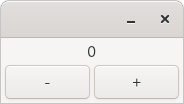
\includegraphics[scale=0.8]{7.png}
    \caption{A simple counting UI}
  \end{figure}

  \begin{Verbatim}[gobble=4,fontsize=\small]
    {-# LANGUAGE ImplicitParams #-}

    module Main (main) where

    import Control.Monad
    import System.Exit
    import qualified Data.Text as Text
    import qualified GI.Gio as G
    import qualified GI.Gtk as Gtk

    main :: IO ()
    main = do
      Just application <- Gtk.applicationNew Nothing [G.ApplicationFlagsDefaultFlags]
      G.onApplicationActivate application onActivate
      status <- G.applicationRun application Nothing
      when (status /= 0) (exitWith (ExitFailure (fromIntegral status)))

    onActivate :: (Gtk.IsApplication a, ?self :: a) => G.ApplicationActivateCallback
    onActivate = do
      label <- Gtk.labelNew (Just (Text.pack "0"))
      buttonMinus  <- Gtk.buttonNewWithLabel (Text.pack "-")
      buttonPlus <- Gtk.buttonNewWithLabel (Text.pack "+")

      buttonBox <- Gtk.buttonBoxNew Gtk.OrientationHorizontal
      Gtk.boxSetSpacing buttonBox 4
      Gtk.containerAdd buttonBox buttonMinus
      Gtk.containerAdd buttonBox buttonPlus

      box <- Gtk.boxNew Gtk.OrientationVertical 4
      Gtk.widgetSetMarginStart box 4
      Gtk.widgetSetMarginEnd box 4
      Gtk.widgetSetMarginTop box 4
      Gtk.widgetSetMarginBottom box 4
      Gtk.containerAdd box label
      Gtk.containerAdd box buttonBox

      window <- Gtk.applicationWindowNew ?self
      Gtk.windowSetTitle window Text.empty
      Gtk.windowSetResizable window False
      Gtk.containerAdd window box

      Gtk.onButtonClicked buttonMinus $ do
        t <- Gtk.labelGetLabel label
        Gtk.labelSetLabel label (Text.pack (show (read (Text.unpack t) - 1)))

      Gtk.onButtonClicked buttonPlus $ do
        t <- Gtk.labelGetLabel label
        Gtk.labelSetLabel label (Text.pack (show (read (Text.unpack t) + 1)))

      Gtk.widgetShowAll window
  \end{Verbatim}

  \vspace{-2pt}

  The entry point \mbox{\texttt{main}} is merely boilerplate code that invokes a
  callback to start the actual application. The window and all its contents are
  constructed in \mbox{\texttt{onActivate}}.

  The first three lines of \mbox{\texttt{onActivate}} create a label initially
  set to \texttt{0} and two buttons: \mbox{\texttt{buttonMinus}} and
  \mbox{\texttt{buttonPlus}}. Note that \mbox{\texttt{gi-gtk}} employs the
  \mbox{\texttt{Text}} data type instead of \mbox{\texttt{String}} for
  efficiency; to convert between the two,
  \mbox{\texttt{Text.pack :: String -> Text}} and
  \mbox{\texttt{Text.unpack :: Text -> String}} have to be used.

  To position the two buttons horizontally, a \mbox{\texttt{Gtk.ButtonBox}}
  container is used. Buttons are added to this container with
  \mbox{\texttt{Gtk.containerAdd}}, and spacing between buttons is configured
  with \mbox{\texttt{Gtk.boxSetSpacing}}.

  To position the button box below the label created earlier, a
  \mbox{\texttt{Gtk.Box}} container is used. Some margin is added on all four
  sides of the container with \mbox{\texttt{Gtk.widgetSetMarginStart}},
  \mbox{\texttt{Gtk.widgetSetMarginEnd}}, \mbox{\texttt{Gtk.widgetSetMarginTop}}
  and \mbox{\texttt{Gtk.widgetSetMarginBottom}}.

  The main window is created with \mbox{\texttt{Gtk.applicationWindowNew}}. Its
  title is set to the empty string, and it is configured to be non-resizable.
  Finally, event handlers for button clicks are registered with
  \mbox{\texttt{Gtk.onButtonClicked}}. Once everything is set up, the
  application window is displayed to the user with
  \mbox{\texttt{Gtk.widgetShowAll}}.

  As demonstrated, using GTK+ within Haskell is not too difficult, even if
  imperative-style programming is required. In most cases, code that works in C
  has an almost direct equivalent in Haskell.

  The package \mbox{\texttt{gi-gtk-hs}} provides an idiomatic API on top of
  \mbox{\texttt{gi-gtk}} which allows loading widgets from XML strings. The
  following listing illustrates an alternative \mbox{\texttt{onActivate}}
  implementation that utilizes this functionality:

  \begin{Verbatim}[gobble=4,fontsize=\small]
    import Data.GI.Gtk.BuildFn

    onActivate' :: (Gtk.IsApplication a, ?self :: a) => G.ApplicationActivateCallback
    onActivate' = do
      let buildFn = do
            label <- getObject Gtk.Label (Text.pack "label")
            buttonMinus <- getObject Gtk.Button (Text.pack "buttonMinus")
            buttonPlus <- getObject Gtk.Button (Text.pack "buttonPlus")
            window <- getObject Gtk.ApplicationWindow (Text.pack "window")

            Gtk.onButtonClicked buttonMinus $ do
              t <- Gtk.labelGetLabel label
              Gtk.labelSetLabel label (Text.pack (show (read (Text.unpack t) - 1)))

            Gtk.onButtonClicked buttonPlus $ do
              t <- Gtk.labelGetLabel label
              Gtk.labelSetLabel label (Text.pack (show (read (Text.unpack t) + 1)))

            pure window
  \end{Verbatim}

  \pagebreak

  \begin{Verbatim}[gobble=4,fontsize=\small]
      let string = Text.pack
            "<interface>\n\
            \  <object class=\"GtkApplicationWindow\" id=\"window\">\n\
            \    <property name=\"title\"></property>\n\
            \    <property name=\"resizable\">false</property>\n\
            \    <child>\n\
            \      <object class=\"GtkBox\">\n\
            \        <property name=\"orientation\">vertical</property>\n\
            \        <property name=\"spacing\">4</property>\n\
            \        <property name=\"margin\">4</property>\n\
            \        <child>\n\
            \          <object class=\"GtkLabel\" id=\"label\">\n\
            \            <property name=\"label\">0</property>\n\
            \          </object>\n\
            \        </child>\n\
            \        <child>\n\
            \          <object class=\"GtkButtonBox\">\n\
            \            <property name=\"orientation\">horizontal</property>\n\
            \            <property name=\"spacing\">4</property>\n\
            \            <child>\n\
            \              <object class=\"GtkButton\" id=\"buttonMinus\">\n\
            \                <property name=\"label\">-</property>\n\
            \              </object>\n\
            \            </child>\n\
            \            <child>\n\
            \              <object class=\"GtkButton\" id=\"buttonPlus\">\n\
            \                <property name=\"label\">+</property>\n\
            \              </object>\n\
            \            </child>\n\
            \          </object>\n\
            \        </child>\n\
            \      </object>\n\
            \    </child>\n\
            \  </object>\n\
            \</interface>"

      builder <- Gtk.builderNewFromString string (fromIntegral (Text.length string))
      window <- buildWithBuilder buildFn builder
      Gtk.windowSetApplication window (Just ?self)
      Gtk.widgetShowAll window
  \end{Verbatim}

  \chapter{Conclusions}

  In this thesis, I demonstrated how to develop an interpreter for a programming
  language from scratch. I explained some of the theory which underlies
  programming languages and gave an introduction to Haskell, which was used to
  implement Devin.

  As for Haskell, I explained how type classes can be encoded as implicit
  parameters; further, I hinted at some of the advantages of type classes over
  interfaces or abstract classes from object-oriented languages. The concept of
  type classes is quite powerful: languages such as Rust and Carbon (Google's
  experimental successor to C++) employ abstractions that can in many ways be
  compared to them. Scala, a language for the JVM, has implicit parameters
  built-in; type classes thus emerge naturally \cite{scala-type-classes}. It
  would be interesting to witness an imperative language that forgoes
  object-orientation completely, opting for a type class like mechanism instead.

  As for Devin, I implemented enough functionality in order to present a good
  starting point for serious programming language implementation: after all,
  Devin only lacks a module system and a standard library. Features such as
  polymorphism and type classes could be added; of course, this would require
  extending the type system and runtime implementations.

  One of the objectives I had for Devin's graphical user interface was to
  illustrate how source code corresponds to syntax trees; with the GTK+ library,
  I developed an interface that not only performs syntax highlighting but also
  visualizes this correspondence. Additionally, Devin's UI implements a
  debugger; with the breakpoint statement, execution can be suspended at
  arbitrary locations, allowing for the program's state to be observed.

  I showed how a monadic mechanism can be used to represent pausable
  computations; more complex solutions might be required in different
  circumstances. Availability of practical material discussing this matter is
  sparse: in fact, implementing debugging functionality has been one of the most
  challenging parts of this whole project.

  Developing Devin has been insightful for gaining a better understanding of the
  matter of programming languages. Actual implementation highlighted the types
  of challenges that arise and require to be solved; using Haskell for such a
  non-trivial project has taught me how to solve problems functionally, while
  providing a new perspective on achieving abstraction through type classes.
  While developing Devin, many ideas for new language constructs arose: in
  particular, the way in which Scala provides and makes use of implicitly passed
  parameters seems to be of great power. I researched which other techniques
  besides monads could be used for achieving side-effects in a purely functional
  way. One possible alternative is to use so-called \emph{algebraic effects}, a
  topic which is subject of ongoing research; languages such as Koka~\cite{koka}
  provide a way of experimenting with such features. With an unbounded amount of
  time at hand, it would've been interesting to develop a purely functional
  language with implicit parameters and an effect system. Alas, this project has
  taken long enough; still, I'm quite satisfied with what I learned from this
  experience.

  \backmatter

  \appendix

  \chapter{Devin source code}
  \label{chapter:devin-source-code}

  \section{\texttt{devin.cabal}}

  \VerbatimInput[fontsize=\footnotesize]{../devin.cabal}
  \vspace{\prevdepth-\depthof{\strut}}

  \section{\texttt{src/Devin/Display.hs}}

  \VerbatimInput[fontsize=\footnotesize]{../src/Devin/Display.hs}
  \vspace{\prevdepth-\depthof{\strut}}

  \section{\texttt{src/Devin/Error.hs}}

  \VerbatimInput[fontsize=\footnotesize]{../src/Devin/Error.hs}
  \vspace{\prevdepth-\depthof{\strut}}

  \section{\texttt{src/Devin/Evaluator.hs}}

  \VerbatimInput[fontsize=\footnotesize]{../src/Devin/Evaluator.hs}
  \vspace{\prevdepth-\depthof{\strut}}

  \section{\texttt{src/Devin/Evaluators.hs}}

  \VerbatimInput[fontsize=\footnotesize]{../src/Devin/Evaluators.hs}
  \vspace{\prevdepth-\depthof{\strut}}

  \section{\texttt{src/Devin/Interval.hs}}

  \VerbatimInput[fontsize=\footnotesize]{../src/Devin/Interval.hs}
  \vspace{\prevdepth-\depthof{\strut}}

  \section{\texttt{src/Devin/Parsec.hs}}

  \VerbatimInput[fontsize=\footnotesize]{../src/Devin/Parsec.hs}
  \vspace{\prevdepth-\depthof{\strut}}

  \section{\texttt{src/Devin/Parsers.hs}}

  \VerbatimInput[fontsize=\footnotesize]{../src/Devin/Parsers.hs}
  \vspace{\prevdepth-\depthof{\strut}}

  \section{\texttt{src/Devin/Ratio.hs}}

  \VerbatimInput[fontsize=\footnotesize]{../src/Devin/Ratio.hs}
  \vspace{\prevdepth-\depthof{\strut}}

  \section{\texttt{src/Devin/Syntax.hs}}

  \VerbatimInput[fontsize=\footnotesize]{../src/Devin/Syntax.hs}
  \vspace{\prevdepth-\depthof{\strut}}

  \section{\texttt{src/Devin/Type.hs}}

  \VerbatimInput[fontsize=\footnotesize]{../src/Devin/Type.hs}
  \vspace{\prevdepth-\depthof{\strut}}

  \section{\texttt{src/Devin/Typer.hs}}

  \VerbatimInput[fontsize=\footnotesize]{../src/Devin/Typer.hs}
  \vspace{\prevdepth-\depthof{\strut}}

  \section{\texttt{src/Devin/Typers.hs}}

  \VerbatimInput[fontsize=\footnotesize]{../src/Devin/Typers.hs}
  \vspace{\prevdepth-\depthof{\strut}}

  \section{\texttt{test/Main.hs}}

  \VerbatimInput[fontsize=\footnotesize]{../test/Main.hs}
  \vspace{\prevdepth-\depthof{\strut}}

  \section{\texttt{test/Devin/EvaluatorsSpec.hs}}

  \VerbatimInput[fontsize=\footnotesize]{../test/Devin/EvaluatorsSpec.hs}
  \vspace{\prevdepth-\depthof{\strut}}

  \section{\texttt{test/Devin/ParsersSpec.hs}}

  \VerbatimInput[fontsize=\footnotesize]{../test/Devin/ParsersSpec.hs}
  \vspace{\prevdepth-\depthof{\strut}}

  \section{\texttt{test/Devin/TypersSpec.hs}}

  \VerbatimInput[fontsize=\footnotesize]{../test/Devin/TypersSpec.hs}
  \vspace{\prevdepth-\depthof{\strut}}

  \section{\texttt{app/Main.hs}}
  \label{section:app-main-hs}

  \VerbatimInput[fontsize=\footnotesize]{../app/Main.hs}
  \vspace{\prevdepth-\depthof{\strut}}

  \section{\texttt{app/Devin/Debug/Evaluator.hs}}

  \VerbatimInput[fontsize=\footnotesize]{../app/Devin/Debug/Evaluator.hs}
  \vspace{\prevdepth-\depthof{\strut}}

  \section{\texttt{app/Devin/Debug/Syntax.hs}}

  \VerbatimInput[fontsize=\footnotesize]{../app/Devin/Debug/Syntax.hs}
  \vspace{\prevdepth-\depthof{\strut}}

  \section{\texttt{app/Devin/Highlight.hs}}

  \VerbatimInput[fontsize=\footnotesize]{../app/Devin/Highlight.hs}
  \vspace{\prevdepth-\depthof{\strut}}

  \section{\texttt{app/Devin/Highlight/Brackets.hs}}

  \VerbatimInput[fontsize=\footnotesize]{../app/Devin/Highlight/Brackets.hs}
  \vspace{\prevdepth-\depthof{\strut}}

  \section{\texttt{app/Devin/Highlight/Syntax.hs}}

  \VerbatimInput[fontsize=\footnotesize]{../app/Devin/Highlight/Syntax.hs}
  \vspace{\prevdepth-\depthof{\strut}}

  \section{\texttt{app/Devin/Levenshtein.hs}}

  \VerbatimInput[fontsize=\footnotesize]{../app/Devin/Levenshtein.hs}
  \vspace{\prevdepth-\depthof{\strut}}

  \printbibliography[heading=bibintoc]
\end{document}
